
\documentclass[11pt,a4paper]{article}

\usepackage[T1]{fontenc}
\usepackage{lmodern}
\usepackage[margin=2.6cm]{geometry}
\usepackage{amsmath,amssymb,bm}
\usepackage{booktabs}
\usepackage{longtable}
\usepackage{array}
\usepackage{graphicx}
\usepackage{xcolor}
\usepackage{listings}
\usepackage{microtype}
\usepackage{enumitem}
\usepackage[hidelinks]{hyperref}
\usepackage{caption}
\usepackage{pgfplots}
\pgfplotsset{compat=1.16}
\usepgfplotslibrary{groupplots}
\graphicspath{{fig/}}
\pgfplotsset{table/search path={fig}}

\definecolor{opBGK}{HTML}{6E7885}
\definecolor{opTRT}{HTML}{A8562A}
\definecolor{opMRT}{HTML}{2D7A8C}
\definecolor{opCM}{HTML}{8B3A62}


\newcommand{\code}[1]{\texttt{\small #1}}
\newcommand{\cs}{c_s}
\newcommand{\ci}{\bm{c}_i}
\newcommand{\uu}{\bm{u}}
\newcommand{\bb}{\bm{b}}
\newcommand{\nn}{\bm{n}}
\newcommand{\xx}{\bm{x}}
\renewcommand{\arraystretch}{1.15}

\captionsetup{font=small,labelfont=bf}

\title{\vspace{-1.4cm}\textbf{LBM\_CODE}\\[2mm]
\large A modular lattice Boltzmann solver on Kokkos\\[1mm]
\normalsize Scheme description, methodology and validation}
\author{}
\date{}

\usepackage{bm}
\newcommand{\e}[1]{\times 10^{#1}}

\begin{document}
\maketitle
\vspace{-1.2cm}

\begin{abstract}
\noindent
This document describes the numerical schemes, the software architecture and the
complete validation record of \code{LBM\_CODE}, a portable lattice Boltzmann
solver written in C\texttt{++}20 on top of Kokkos. The code targets NVIDIA GPUs
and CPU clusters from a single source. It supports five lattices, two streaming
schemes (including the in-place Esoteric Pull), two population storage
conventions, four collision operators for the fluid (BGK, TRT, raw multiple
relaxation time and central moments), a passive-scalar module for heat transfer
and a magnetohydrodynamic module built on a vector-valued distribution. Every
scheme documented here is accompanied by the quantitative test that establishes
it, and every stated limitation is one that has been measured rather than
assumed.
\end{abstract}

\tableofcontents
\bigskip
\hrule

%==============================================================================
\section{Scope and design}

\subsection{What the code is}

\code{LBM\_CODE} solves the weakly compressible Navier--Stokes equations by the
lattice Boltzmann method, optionally coupled to a passive scalar (temperature)
and to a magnetic field. It is written once and compiled for any Kokkos backend:
Serial, Threads, OpenMP, CUDA, HIP or SYCL. Scalar precision is selected at
configure time.

\subsection{Governing equations}

The fluid obeys
\begin{align}
  \partial_t \rho + \nabla\!\cdot(\rho\uu) &= 0, \\
  \partial_t(\rho\uu) + \nabla\!\cdot(\rho\uu\uu)
     &= -\nabla p + \nabla\!\cdot\bm{\tau} + \bm{F},
\end{align}
with $p=\rho\cs^2$ and $\bm{\tau}$ the viscous stress. When the thermal module is
active a scalar $T$ is transported by
\begin{equation}
  \partial_t T + \nabla\!\cdot(\uu T) = D\,\nabla^2 T ,
\end{equation}
and couples back to the flow through the Boussinesq body force. When the
magnetohydrodynamic module is active the magnetic field $\bb$ obeys the induction
equation
\begin{equation}
  \partial_t \bb = \nabla\times(\uu\times\bb) + \eta\,\nabla^2\bb,
  \qquad \nabla\!\cdot\bb = 0,
  \label{eq:induction}
\end{equation}
and acts on the flow through the Lorentz force $\bm{j}\times\bb$ with
$\bm{j}=\nabla\times\bb$.

\subsection{Architectural rules}
\label{sec:rules}

Seven rules govern the implementation. They are stated here because most of the
design decisions in later sections follow from them rather than from the physics.

\begin{enumerate}[leftmargin=1.4em,itemsep=3pt]
\item \textbf{No virtual functions in device code.} Lattice, streaming scheme,
  equilibrium, forcing, storage convention and collision operator are all
  compile-time policies that inline into a single kernel. Dynamic dispatch exists
  only in a host-side factory above the solver. A virtual call inside a Kokkos
  kernel runs, but it blocks inlining of the entire collision operator.

\item \textbf{Never pin the Kokkos memory layout.} Population fields are declared
  \code{View<Real**>} with extents \code{(node, q)} and the \emph{default} layout.
  Kokkos then selects \code{LayoutLeft} on CUDA/HIP --- node index fastest, hence
  a structure of arrays with coalesced access --- and \code{LayoutRight} on
  CPU backends, giving an array of structures with good cache locality per node.
  One declaration is correct on both; hardcoding either costs performance on the
  other.

\item \textbf{Streaming and collision are one fused kernel.} The in-place
  streaming schemes cannot have a separate streaming pass, so nothing in the
  solver is written in a way that would assume one.

\item \textbf{Parity is a compile-time parameter.} Esoteric Pull addresses
  different storage slots on even and odd time steps. That decision must fold
  away at compile time, so \code{FluidSolver::step} dispatches to
  \code{run\_step<0>} or \code{run\_step<1>}.

\item \textbf{Periodicity is index wrapping, not halo copying.} See
  \S\ref{sec:periodic}.

\item \textbf{Boundary conditions are alternative collision operators} applied to
  flagged cells, giving one branch per node rather than one per direction.

\item \textbf{The reference implementation is never deleted.} The two-lattice
  streaming scheme is retained permanently and cross-checked against Esoteric
  Pull after every step.
\end{enumerate}

%==============================================================================
\section{Lattices}

\subsection{Definition and constraints}

A lattice is a set of $Q$ velocities $\ci$ with weights $w_i$ and a lattice sound
speed $\cs$. To recover the Navier--Stokes equations at second order the set must
satisfy
\begin{align}
  \textstyle\sum_i w_i &= 1, &
  \textstyle\sum_i w_i c_{i\alpha} c_{i\beta} &= \cs^2\delta_{\alpha\beta},
  \label{eq:iso2}\\
  \textstyle\sum_i w_i c_{i\alpha} c_{i\beta} c_{i\gamma} &= 0, &
  \textstyle\sum_i w_i c_{i\alpha} c_{i\beta} c_{i\gamma} c_{i\delta}
    &= \cs^4\big(\delta_{\alpha\beta}\delta_{\gamma\delta}
      + \delta_{\alpha\gamma}\delta_{\beta\delta}
      + \delta_{\alpha\delta}\delta_{\beta\gamma}\big).
  \label{eq:iso4}
\end{align}

Five lattices are provided. \textbf{D2Q5} and \textbf{D3Q7} satisfy
\eqref{eq:iso2} but \emph{not} \eqref{eq:iso4}: they cannot support
Navier--Stokes and are used only for scalar transport and for the magnetic field,
where only the second moment is required.

\begin{table}[h]
\centering\small
\begin{tabular}{lccccc}
\toprule
lattice & $Q$ & $D$ & $\cs^2$ & weights & Navier--Stokes \\
\midrule
D2Q5  & 5  & 2 & $1/3$ & $1/3;\ 1/6$ & no \\
D2Q9  & 9  & 2 & $1/3$ & $4/9;\ 1/9;\ 1/36$ & yes \\
D3Q7  & 7  & 3 & $1/4$ & $1/4;\ 1/8$ & no \\
D3Q27 & 27 & 3 & $1/3$ & $8/27;\ 2/27;\ 1/54;\ 1/216$ & yes \\
\bottomrule
\end{tabular}
\caption{The four lattices. Note that D3Q7 has $\cs^2=1/4$, not $1/3$.}
\end{table}

\subsection{Velocity sets}
\label{sec:velsets}

The complete velocity sets follow, in the Esoteric Pull ordering of
\S\ref{sec:ordering}. These tables are generated from the same data the code
compiles against, and the identities in the captions are re-verified in exact
rational arithmetic at generation time.

\begin{table}[t]
\centering\small
\begin{tabular}{r c c c r c c c }
\toprule
$i$ & $\ci$ & $w_i$ & opp & $i$ & $\ci$ & $w_i$ & opp \\
\midrule
0 & $(0,0)$ & $\tfrac{1}{3}$ & 0 & 3 & $(0,1)$ & $\tfrac{1}{6}$ & 4 \\
1 & $(1,0)$ & $\tfrac{1}{6}$ & 2 & 4 & $(0,-1)$ & $\tfrac{1}{6}$ & 3 \\
2 & $(-1,0)$ & $\tfrac{1}{6}$ & 1 &  & & &  \\
\bottomrule
\end{tabular}
\caption{\textbf{D2Q5}: velocity set in the Esoteric Pull ordering
(\S\ref{sec:ordering}), weights, and $\mathrm{opp}(i)$. $\cs^2=\tfrac{1}{3}$.
Verified: $\sum_i w_i=1$ and $\sum_i w_i c_{i\alpha}c_{i\beta}=\cs^2\delta_{\alpha\beta}$
in exact rational arithmetic.}
\end{table}

\begin{table}[t]
\centering\small
\begin{tabular}{r c c c r c c c }
\toprule
$i$ & $\ci$ & $w_i$ & opp & $i$ & $\ci$ & $w_i$ & opp \\
\midrule
0 & $(0,0)$ & $\tfrac{4}{9}$ & 0 & 5 & $(1,1)$ & $\tfrac{1}{36}$ & 6 \\
1 & $(1,0)$ & $\tfrac{1}{9}$ & 2 & 6 & $(-1,-1)$ & $\tfrac{1}{36}$ & 5 \\
2 & $(-1,0)$ & $\tfrac{1}{9}$ & 1 & 7 & $(1,-1)$ & $\tfrac{1}{36}$ & 8 \\
3 & $(0,1)$ & $\tfrac{1}{9}$ & 4 & 8 & $(-1,1)$ & $\tfrac{1}{36}$ & 7 \\
4 & $(0,-1)$ & $\tfrac{1}{9}$ & 3 &  & & &  \\
\bottomrule
\end{tabular}
\caption{\textbf{D2Q9}: velocity set in the Esoteric Pull ordering
(\S\ref{sec:ordering}), weights, and $\mathrm{opp}(i)$. $\cs^2=\tfrac{1}{3}$.
Verified: $\sum_i w_i=1$ and $\sum_i w_i c_{i\alpha}c_{i\beta}=\cs^2\delta_{\alpha\beta}$
in exact rational arithmetic.}
\end{table}

\begin{table}[t]
\centering\small
\begin{tabular}{r c c c r c c c }
\toprule
$i$ & $\ci$ & $w_i$ & opp & $i$ & $\ci$ & $w_i$ & opp \\
\midrule
0 & $(0,0,0)$ & $\tfrac{1}{4}$ & 0 & 4 & $(0,-1,0)$ & $\tfrac{1}{8}$ & 3 \\
1 & $(1,0,0)$ & $\tfrac{1}{8}$ & 2 & 5 & $(0,0,1)$ & $\tfrac{1}{8}$ & 6 \\
2 & $(-1,0,0)$ & $\tfrac{1}{8}$ & 1 & 6 & $(0,0,-1)$ & $\tfrac{1}{8}$ & 5 \\
3 & $(0,1,0)$ & $\tfrac{1}{8}$ & 4 &  & & &  \\
\bottomrule
\end{tabular}
\caption{\textbf{D3Q7}: velocity set in the Esoteric Pull ordering
(\S\ref{sec:ordering}), weights, and $\mathrm{opp}(i)$. $\cs^2=\tfrac{1}{4}$.
Verified: $\sum_i w_i=1$ and $\sum_i w_i c_{i\alpha}c_{i\beta}=\cs^2\delta_{\alpha\beta}$
in exact rational arithmetic.}
\end{table}

\begin{table}[t]
\centering\small
\begin{tabular}{r c c c r c c c r c c c }
\toprule
$i$ & $\ci$ & $w_i$ & opp & $i$ & $\ci$ & $w_i$ & opp & $i$ & $\ci$ & $w_i$ & opp \\
\midrule
0 & $(0,0,0)$ & $\tfrac{8}{27}$ & 0 & 9 & $(1,-1,0)$ & $\tfrac{1}{54}$ & 10 & 18 & $(0,-1,1)$ & $\tfrac{1}{54}$ & 17 \\
1 & $(1,0,0)$ & $\tfrac{2}{27}$ & 2 & 10 & $(-1,1,0)$ & $\tfrac{1}{54}$ & 9 & 19 & $(1,1,1)$ & $\tfrac{1}{216}$ & 20 \\
2 & $(-1,0,0)$ & $\tfrac{2}{27}$ & 1 & 11 & $(1,0,1)$ & $\tfrac{1}{54}$ & 12 & 20 & $(-1,-1,-1)$ & $\tfrac{1}{216}$ & 19 \\
3 & $(0,1,0)$ & $\tfrac{2}{27}$ & 4 & 12 & $(-1,0,-1)$ & $\tfrac{1}{54}$ & 11 & 21 & $(1,1,-1)$ & $\tfrac{1}{216}$ & 22 \\
4 & $(0,-1,0)$ & $\tfrac{2}{27}$ & 3 & 13 & $(1,0,-1)$ & $\tfrac{1}{54}$ & 14 & 22 & $(-1,-1,1)$ & $\tfrac{1}{216}$ & 21 \\
5 & $(0,0,1)$ & $\tfrac{2}{27}$ & 6 & 14 & $(-1,0,1)$ & $\tfrac{1}{54}$ & 13 & 23 & $(1,-1,1)$ & $\tfrac{1}{216}$ & 24 \\
6 & $(0,0,-1)$ & $\tfrac{2}{27}$ & 5 & 15 & $(0,1,1)$ & $\tfrac{1}{54}$ & 16 & 24 & $(-1,1,-1)$ & $\tfrac{1}{216}$ & 23 \\
7 & $(1,1,0)$ & $\tfrac{1}{54}$ & 8 & 16 & $(0,-1,-1)$ & $\tfrac{1}{54}$ & 15 & 25 & $(-1,1,1)$ & $\tfrac{1}{216}$ & 26 \\
8 & $(-1,-1,0)$ & $\tfrac{1}{54}$ & 7 & 17 & $(0,1,-1)$ & $\tfrac{1}{54}$ & 18 & 26 & $(1,-1,-1)$ & $\tfrac{1}{216}$ & 25 \\
\bottomrule
\end{tabular}
\caption{\textbf{D3Q27}: velocity set in the Esoteric Pull ordering
(\S\ref{sec:ordering}), weights, and $\mathrm{opp}(i)$. $\cs^2=\tfrac{1}{3}$.
Verified: $\sum_i w_i=1$ and $\sum_i w_i c_{i\alpha}c_{i\beta}=\cs^2\delta_{\alpha\beta}$
in exact rational arithmetic.}
\end{table}

\subsection{The direction-ordering contract}
\label{sec:ordering}

Esoteric Pull walks opposite pairs as \code{for (i = 1; i < Q; i += 2)}. This
requires that the rest velocity occupies index $0$ and that opposite directions
occupy \emph{adjacent} indices, so that
\begin{equation}
  \mathrm{opp}(0)=0, \qquad
  \mathrm{opp}(i) = \begin{cases} i+1 & i \text{ odd} \\ i-1 & i \text{ even}\end{cases}
  \label{eq:opp}
\end{equation}
is pure integer arithmetic, with no lookup table in the kernel. This is a
\emph{contract}: every moment matrix in the code is generated against it.

Reordering the directions of a lattice is a column permutation of the moment
transform matrices together with the matching permutation of $f_i$ and
$f_i^{\rm eq}$. Every moment, raw or central, is therefore invariant, and only
the per-direction post-collision expressions are permuted. This was verified
numerically in exact rational arithmetic before the orderings were adopted.

\subsection{Compile-time verification}

Weights are stored as exact rationals ($w_i = \code{w\_num}[i]/\code{w\_den}$) and
$\cs^2$ as \code{cs2\_num/cs2\_den}, so all the identities above are checked at
compile time in exact integer arithmetic rather than in floating point:

\begin{lstlisting}[basicstyle=\ttfamily\scriptsize]
static_assert(check_pairing<L>(),       "opposite directions not adjacent");
static_assert(check_unique<L>(),        "duplicated velocity");
static_assert(check_w_sum<L>(),         "weights do not sum to 1");
static_assert(check_second_moment<L>(), "<cc> != cs2 I");
static_assert(check_third_moment<L>(),  "<ccc> != 0");
static_assert(check_fourth_moment<L>() == L::supports_navier_stokes, "");
\end{lstlisting}

The last line is an equality rather than a truth test: D2Q5 and D3Q7 are
\emph{required} to fail fourth-order isotropy, and a lattice whose flag disagrees
with its actual moments will not compile.

%==============================================================================
\section{Streaming}

\subsection{Two-lattice (reference)}

Two arrays, $2Q$ reals per node. Semantics are \emph{pull}: the kernel gathers
the populations that have arrived at node $n$,
\begin{equation}
  f_i^{\rm in}(n) = f_i^{\rm src}(n - \ci),
\end{equation}
collides, and writes locally to the destination array, which is then swapped.
This scheme is obviously race-free and obviously correct. It is not the
production scheme, but it is retained permanently: when an exotic collision
operator produces incorrect results, being able to switch to a streaming scheme
that cannot be wrong is what makes the fault bisectable.

\subsection{Esoteric Pull}
\label{sec:esopull}

Esoteric Pull \cite{lehmann2022} stores a single copy of the populations and
updates them in place. Write $A[n][s]$ for storage slot $s$ at node $n$, and
consider one opposite pair $(i,i+1)$ with $i$ odd. The partner node is
\emph{always} $n+\ci$, at both parities; only which of the two slots lives
remotely alternates.

\begin{table}[h]
\centering\small
\begin{tabular}{ll}
\toprule
even step $t$ & odd step $t$ \\
\midrule
$f_i \leftarrow A[n][i]$              & $f_i \leftarrow A[n][i{+}1]$ \\
$f_{i+1} \leftarrow A[n+\ci][i{+}1]$  & $f_{i+1} \leftarrow A[n+\ci][i]$ \\
$A[n+\ci][i{+}1] \leftarrow f_i^{\rm out}$ & $A[n+\ci][i] \leftarrow f_i^{\rm out}$ \\
$A[n][i] \leftarrow f_{i+1}^{\rm out}$     & $A[n][i{+}1] \leftarrow f_{i+1}^{\rm out}$ \\
\bottomrule
\end{tabular}
\caption{The Esoteric Pull access pattern, one opposite pair. Each parity reads
exactly two slots and writes those same two, crossed.}
\label{tab:esopull}
\end{table}

\paragraph{Consistency.} At an even step node $n$ writes its outgoing $f_i$ into
$A[n+\ci][i{+}1]$; at the next (odd) step node $m=n+\ci$ reads $f_i$ from
$A[m][i{+}1]$, which is exactly the odd-step rule. The scheme closes.

\paragraph{Race freedom.} Every slot has exactly one reader and one writer, and
they are the same node. No temporary buffer and no synchronisation within a step
are required.

\paragraph{Implicit bounce-back.} Halfway bounce-back sets
$f_i^{\rm out}=f_{i+1}^{\rm in}$ and $f_{i+1}^{\rm out}=f_i^{\rm in}$.
Substituting into Table~\ref{tab:esopull}, every write lands back in the slot it
was read from: the entire update is the identity. \emph{Solid cells are therefore
skipped outright} --- no load, no store, no arithmetic. The population a fluid
node emits toward a wall sits untouched for one step and is read back as the
opposite direction on the next, placing the wall exactly midway between the two
cells.

\paragraph{Memory.} $Q$ reals per node against $2Q$ for two-lattice. At
$512^3$ with D3Q27 in FP64 this is the difference between $29$\,GB and $58$\,GB,
i.e.\ between fitting and not fitting on a 40\,GB device.

\subsection{Periodicity by index wrapping}
\label{sec:periodic}

Esoteric Pull writes into its neighbours' storage. A halo-copy treatment of
periodicity would therefore require a \emph{two-way} exchange whose set of
exchanged slots depends on the parity. The code instead resolves periodicity by
wrapping the neighbour index, which removes that entire class of bug:
\begin{equation}
  \mathrm{shift}(v) =
  \begin{cases}
    v+n & v < h \\ v-n & v \geq h+n \\ v & \text{otherwise}
  \end{cases}
  \quad\text{(periodic)}, \qquad
  \mathrm{clamp}(v,0,s-1) \quad\text{(otherwise)}.
\end{equation}
A halo layer is allocated only in non-periodic directions, where edge cells
genuinely need somewhere out-of-domain to read from. A fast path skips the
wrapping entirely for nodes away from every face.

%==============================================================================
\section{Population storage}
\label{sec:storage}

Two conventions are supported.

\begin{description}[leftmargin=1.6em]
\item[Raw] the arrays hold $f_i$.
\item[Shifted] the arrays hold $g_i = f_i - w_i$.
\end{description}

The shift exists for conditioning. Populations are $O(w_i)\sim10^{-1}$, while the
collision operates on differences $O(10^{-6})$; forming $f_i - f_i^{\rm eq}$ in
FP32 therefore discards most of the mantissa. The momentum sum is worse, since
$\sum_i \ci f_i$ cancels terms of order $10^{-1}$ down to $10^{-2}$. Storing
$g_i$ removes both cancellations, because $\sum_i \ci w_i = 0$ exactly and hence
\begin{equation}
  \sum_i \ci\, g_i \;\equiv\; \sum_i \ci\, f_i
\end{equation}
identically, while every summand is small. The density follows from
$\rho = 1 + \sum_i g_i$.

Almost nothing else changes. Streaming is a pure copy and is untouched. Halfway
bounce-back is $g_i \leftarrow g_{\mathrm{opp}(i)}$, untouched, because
$w_i = w_{\mathrm{opp}(i)}$. The Guo source term is already an $O(F)$ quantity and
is untouched. Only the equilibrium and the density reconstruction differ.

\medskip
\noindent\textbf{Measured effect.} Poiseuille flow at the magic relaxation time,
$H=32$, in FP32:

\begin{center}\small
\begin{tabular}{lcc}
\toprule
storage & FP64 & FP32 \\
\midrule
raw     & $1.433\times10^{-13}$ & $5.969\times10^{-4}$ \\
shifted & $1.626\times10^{-14}$ & $\bm{2.778\times10^{-5}}$ \\
\midrule
gain    & $8.8\times$ & $\bm{21.5\times}$ \\
\bottomrule
\end{tabular}
\end{center}

\noindent The validation suite asserts that gain rather than merely tolerating
its absence: a regression to raw storage fails the build.

For the passive scalar the same argument applies but there is \emph{no universal
reference}. Density is always near unity; a temperature scale is whatever the
problem says it is. The scalar collision therefore exposes $T_{\rm ref}$ as a
runtime parameter, defaulting to $0$, which reproduces unshifted storage exactly.


%==============================================================================
\section{Equilibria}
\label{sec:equilibria}

This section states, for every lattice, the equilibrium that the code actually
evaluates. The distinction matters in one place in particular: the moment-space
operators of \S\ref{sec:moment} \emph{never form equilibrium populations at all}.
Their equilibrium is defined directly in moment space, and the corresponding
populations exist only implicitly, as the inverse transform of those moments.

\subsection{The $\phi$ formulation}
\label{sec:eqphi}

Each populations-space equilibrium policy supplies only $\phi_i(\uu)$, defined by
\begin{equation}
  f_i^{\rm eq} = w_i\,\rho\,(1+\phi_i),
\end{equation}
from which both storage conventions of \S\ref{sec:storage} follow once:
\begin{align}
  \text{raw:}     &\quad f_i^{\rm eq}       = w_i\,\rho\,(1+\phi_i), \\
  \text{shifted:} &\quad f_i^{\rm eq} - w_i = w_i\big(\delta\rho + (1+\delta\rho)\,\phi_i\big),
  \qquad \delta\rho = \rho-1 .
  \label{eq:eqshift}
\end{align}
Form \eqref{eq:eqshift} is written that way deliberately: every term is small, so
it never forms the difference of two $O(w_i)$ quantities. Writing it as
$f_i^{\rm eq}-w_i$ would be algebraically identical and numerically useless.

\subsection{Second-order (truncated Hermite) --- D2Q9, D3Q27}
\label{sec:eq2}

The default for BGK, TRT and the MHD fluid operator, on all three
Navier--Stokes lattices:
\begin{equation}
  \boxed{\;
  f_i^{\rm eq} = w_i\,\rho\left[
      1 + \frac{\ci\!\cdot\!\uu}{\cs^2}
        + \frac{(\ci\!\cdot\!\uu)^2}{2\cs^4}
        - \frac{\uu\!\cdot\!\uu}{2\cs^2}\right] \;}
  \label{eq:so}
\end{equation}
With $\cs^2=1/3$ on all three, this is
$f_i^{\rm eq}=w_i\rho\big[1+3(\ci\!\cdot\!\uu)+\tfrac92(\ci\!\cdot\!\uu)^2-\tfrac32\uu^2\big]$.
It is correct to $O(u^2)$; its central moments carry $O(u^3)$ defects, which is
what the Galilean-invariance test of \S\ref{sec:galilean} measures and what the
moment operators remove.

\subsection{Product form --- D2Q9 and D3Q27}
\label{sec:eqprod}

The complete (fourth-order) equilibrium, equivalent to
\code{index\_equilibrium = 4} of the symbolic generator. Writing
$a_\alpha = c_{i\alpha}^2-\cs^2$,
\begin{equation}
  \boxed{\;
  \begin{aligned}
  f_i^{\rm eq} = w_i\rho\Big[1
    &+ \frac{c_{ix}u_x+c_{iy}u_y}{\cs^2}
     + \frac{a_x u_x^2 + a_y u_y^2 + 2c_{ix}c_{iy}u_xu_y}{2\cs^4} \\
    &+ \frac{a_x c_{iy} u_x^2 u_y + a_y c_{ix} u_x u_y^2}{2\cs^6}
     + \frac{a_x a_y\, u_x^2 u_y^2}{4\cs^8}\Big]
  \end{aligned}\;}
  \label{eq:prod9}
\end{equation}
Its central moments are \emph{exactly} Maxwellian for all nine representable
$k_{pq}$ --- verified symbolically, 0 of 9 deviating --- so it is fully Galilean
invariant on this lattice.

\medskip
\noindent\textbf{D3Q27: sixth order.} D3Q27 is a product lattice, so the same
construction runs to sixth order --- the highest its 27 velocities admit. The
symbolic generator writes it as a sum of Hermite tensors of orders one to six.
That sum was checked, in exact rational arithmetic, against the factorised form
\begin{equation}
  \boxed{\;
  f_i^{\rm eq} = \rho\,\psi(c_{ix},u_x)\,\psi(c_{iy},u_y)\,\psi(c_{iz},u_z),
  \qquad
  \begin{aligned}
    \psi(0,u)     &= 1-\cs^2-u^2, \\
    \psi(\pm1,u)  &= \tfrac12\big(\cs^2+u^2\pm u\big),
  \end{aligned}\;}
  \label{eq:prod27}
\end{equation}
and the two are \emph{identical, term for term}. The one-dimensional factor
$\psi$ is simply the three-point distribution carrying the exact moments
$\{1,\,u,\,\cs^2+u^2\}$. Equation \eqref{eq:prod27} is what the code evaluates:
three multiplications instead of six Hermite tensors, bit-for-bit the same
polynomial. Dividing each factor by its one-dimensional weight
$\{\tfrac16,\tfrac23,\tfrac16\}$ puts it in the $\phi$ form of \S\ref{sec:eqphi},
since $w_i = w^{\rm 1D}(c_{ix})w^{\rm 1D}(c_{iy})w^{\rm 1D}(c_{iz})$ on a product
lattice:
\begin{equation}
  \phi_i = \chi(c_{ix},u_x)\,\chi(c_{iy},u_y)\,\chi(c_{iz},u_z) - 1,
  \qquad
  \chi(0,u) = 1-\tfrac32u^2,\quad \chi(\pm1,u) = 1+3u(\pm1+u).
  \label{eq:chi27}
\end{equation}

\medskip
\noindent\textbf{The defining property.} The central moments of
\eqref{eq:prod9} and \eqref{eq:prod27} are \emph{exactly} Maxwellian in every
representable moment:
\begin{equation}
  k_{pqr}^{\rm eq} =
  \begin{cases}
    \rho\,(\cs^2)^{\,n}, & p,q,r \text{ all even},\ n = \#\{p,q,r\ \text{equal to } 2\}, \\[2pt]
    0, & \text{otherwise},
  \end{cases}
  \label{eq:maxcm}
\end{equation}
so 8 of the 27 D3Q27 moments are nonzero and the remaining 19 vanish identically.
Every Galilean-invariance defect of the truncation \eqref{eq:so} is absent.

\noindent\textbf{Where these are used.} \eqref{eq:prod9} and \eqref{eq:prod27}
are collected as \code{HighOrderEquilibrium<L>}, which selects the highest order
each lattice admits. This is the default for the MHD operators
of \S\ref{sec:mhdcm}. The BGK and TRT defaults remain \eqref{eq:so}, and the
moment-space operators of \S\ref{sec:eqmom} reach the same equilibrium without
evaluating any of these forms explicitly.

\subsection{Equilibria in moment space --- D2Q9, D3Q27}
\label{sec:eqmom}

The MRT and central-moment operators specify their equilibrium as \emph{moments},
in closed form. Writing $\uu_b$ for the basis velocity ($\bm0$ for raw moments,
$\uu$ for central) and $\delta\uu = \uu-\uu_b$, the equilibrium moment in the
stored variable is a product of one-dimensional factors,
\begin{equation}
  \boxed{\;
  E_{pqr} = \rho\;Q_p(\delta u_x)\,Q_q(\delta u_y)\,Q_r(\delta u_z)
   \;-\;[\text{shifted}]\;A_p(u_{bx})\,A_q(u_{by})\,A_r(u_{bz})\;}
  \label{eq:emom}
\end{equation}
with the triples depending on which basis the lattice uses:

\begin{center}\small
\begin{tabular}{llll}
\toprule
lattice & basis & $Q_{0,1,2}$ & $A_{0,1,2}$ \\
\midrule
D2Q9, D3Q27 & product, $\varphi_2=C^2-\cs^2$ &
  $1,\ \delta u,\ \delta u^2$ & $1,\ -u_b,\ u_b^2$ \\
\bottomrule
\end{tabular}
\end{center}

\noindent Two consequences are worth stating explicitly.

\paragraph{Central moments on D2Q9 and D3Q27.} Here $\delta\uu=\bm0$, so
$Q=(1,0,0)$ and \eqref{eq:emom} collapses to
\begin{equation}
  E_{0\ldots0} = \rho, \qquad E_{pqr} = 0 \ \ \text{otherwise}
  \qquad\text{(raw storage)} .
\end{equation}
\emph{One nonzero equilibrium moment.} This is the property that makes the
operator cheap: no equilibrium populations, no stored $K^{\rm eq}$ vector, no
$Q\times Q$ matrices. It was verified symbolically --- 0 of 9 deviating on D2Q9,
0 of 27 on D3Q27 --- and it is equivalent to relaxing toward \eqref{eq:prod9} and
its D3Q27 counterpart.

\paragraph{Raw MRT.} Here $\uu_b=\bm0$ and $\delta\uu=\uu$, so
$Q=(1,u,u^2)$ on the product basis and $(1,u,\cs^2+u^2)$ on the monomial one ---
the raw moments of a Maxwellian centred on $\uu$. Note this gives raw MRT the
\emph{complete} equilibrium, not a truncated one, which is why it recovers most
of the Galilean-invariance gain on its own (\S\ref{sec:galilean}).

\subsection{Scalar transport --- D2Q5, D3Q7}
\label{sec:eqscalar}

The passive scalar carries only its zeroth moment, $T=\sum_i g_i$, and is
advected by a velocity supplied from outside:
\begin{equation}
  \boxed{\; g_i^{\rm eq} = w_i\,T\left(1+\frac{\ci\!\cdot\!\uu}{\cs^2}\right)\;}
  \qquad
  D = \cs^2\Big(\frac{1}{\omega}-\frac12\Big).
  \label{eq:eqad}
\end{equation}
Explicitly, with $\cs^2=1/3$ on D2Q5 and $\cs^2=1/4$ on D3Q7,
\begin{align}
  \text{D2Q5:}&\quad g_i^{\rm eq} = w_i T\big(1+3\,\ci\!\cdot\!\uu\big),
     & w &= \big(\tfrac13;\ \tfrac16,\tfrac16,\tfrac16,\tfrac16\big), \\
  \text{D3Q7:}&\quad g_i^{\rm eq} = w_i T\big(1+4\,\ci\!\cdot\!\uu\big),
     & w &= \big(\tfrac14;\ \tfrac18\ \text{(six times)}\big).
\end{align}
In the shifted storage of \S\ref{sec:storage} the code evaluates
\begin{equation}
  h_i^{\rm eq} = w_i\left[\delta T + (T_{\rm ref}+\delta T)\,
    \frac{\ci\!\cdot\!\uu}{\cs^2}\right], \qquad \delta T = T-T_{\rm ref},
\end{equation}
which is \eqref{eq:eqad} minus $w_iT_{\rm ref}$, written so that no term is the
difference of two $O(w_iT)$ quantities.

\paragraph{Why first order.} The truncation in \eqref{eq:eqad} is deliberate.
D2Q5 and D3Q7 have an isotropic second moment but not an isotropic fourth-order
one, and on D3Q7 every velocity has a single nonzero component, so
$(\ci\!\cdot\!\uu)^2$ reduces to $c_\alpha^2u_\alpha^2$ and the cross terms of the
$\uu\uu$ tensor cannot be represented at all. A second-order term would add an
anisotropic error rather than accuracy. The cost is an $O(u^2)$ defect in the
advection term, which is why these lattices suit low-Mach transport.

\subsection{Magnetic induction --- D2Q5, D3Q7}
\label{sec:eqmag}

The magnetic field is carried by a distribution that is a \emph{vector} at every
link, with $b_\alpha=\sum_i g_i^\alpha$:
\begin{equation}
  \boxed{\;
  g_i^{{\rm eq},\alpha} = w_i\left[b_\alpha
    + \frac{c_{i\beta}}{\cs^2}\big(u_\beta b_\alpha - b_\beta u_\alpha\big)\right]\;}
  \qquad
  \eta = \cs^2\Big(\frac{1}{\omega_\eta}-\frac12\Big).
  \label{eq:eqmag}
\end{equation}
Its first two moments are $\sum_i g_i^{\rm eq,\alpha}=b_\alpha$ and
$\sum_i c_{i\beta}g_i^{{\rm eq},\alpha}=u_\beta b_\alpha - b_\beta u_\alpha$,
which is exactly the antisymmetric flux of the induction equation. Only that
first moment is required, which is why a five- or seven-velocity lattice suffices
for the field while the flow runs on nine, nineteen or twenty-seven.

\subsection{MHD fluid equilibrium --- D2Q9, D3Q27}
\label{sec:eqmhd}

The Lorentz force enters through the equilibrium's second moment rather than as a
body force. To \eqref{eq:so} is added
\begin{equation}
  \boxed{\;
  \delta f_i = \frac{w_i}{2\cs^4}\,M_{\alpha\beta}
    \big(c_{i\alpha}c_{i\beta} - \cs^2\delta_{\alpha\beta}\big),
  \qquad
  M_{\alpha\beta} = \tfrac12|\bb|^2\delta_{\alpha\beta} - b_\alpha b_\beta \;}
  \label{eq:eqmaxwell}
\end{equation}
so that $\sum_i c_{i\alpha}c_{i\beta}f_i^{\rm eq}
= \rho u_\alpha u_\beta + (p+\tfrac12|\bb|^2)\delta_{\alpha\beta} - b_\alpha b_\beta$,
while $\sum_i\delta f_i=0$ and $\sum_i\ci\,\delta f_i=\bm0$ leave mass and
momentum untouched.

\medskip
\noindent\textbf{Dimensional form.} In two dimensions
$M_{\alpha\beta}\delta_{\alpha\beta}=|\bb|^2-|\bb|^2=0$, so \eqref{eq:eqmaxwell}
reduces to the familiar
\begin{equation}
  \delta f_i = \frac{w_i}{2\cs^4}
    \Big[\tfrac12|\ci|^2|\bb|^2 - (\ci\!\cdot\!\bb)^2\Big]
  \qquad\text{(2D only)} .
\end{equation}
In three dimensions $M_{\alpha\beta}\delta_{\alpha\beta}=\tfrac12|\bb|^2\neq0$ and
the trace subtraction is retained. This is not cosmetic: it is precisely the term
whose projection onto the plane governs the quasi-two-dimensional reduction test
of \S\ref{sec:reduction}.

\subsection{Summary: which equilibrium is used where}
\label{sec:eqsummary}

\begin{center}\small
\begin{tabular}{llll}
\toprule
operator & lattices & equilibrium & where \\
\midrule
BGK, TRT            & D2Q9, D3Q27 & second order, \eqref{eq:so} & \S\ref{sec:eq2} \\
MRT (raw moments)   & D2Q9, D3Q27 & moment space, \eqref{eq:emom}, $\uu_b=\bm0$ & \S\ref{sec:eqmom} \\
central moments     & D2Q9, D3Q27 & moment space, \eqref{eq:emom}, $\uu_b=\uu$ & \S\ref{sec:eqmom} \\
MHD fluid (BGK)     & D2Q9, D3Q27 & \eqref{eq:so} $+$ \eqref{eq:eqmaxwell} & \S\ref{sec:eqmhd} \\
MHD central moments & D2Q9               & \eqref{eq:prod9} $+$ \eqref{eq:eqmaxwell}; CMs \eqref{eq:cmeqho} & \S\ref{sec:mhdcm} \\
                    & D3Q27              & \eqref{eq:prod27} $+$ \eqref{eq:eqmaxwell}; CMs \eqref{eq:cm3dho} & \S\ref{sec:mhdcm3d} \\
                    & \emph{(\code{-eq2})} & second order \eqref{eq:so}; CMs \eqref{eq:cmeq} & \S\ref{sec:mhdcm} \\
scalar transport    & D2Q5, D3Q7         & first order, \eqref{eq:eqad} & \S\ref{sec:eqscalar} \\
magnetic induction  & D2Q5, D3Q7         & Dellar, \eqref{eq:eqmag} & \S\ref{sec:eqmag} \\
\midrule
\multicolumn{4}{l}{\emph{highest order each lattice admits:} \eqref{eq:prod9} D2Q9, \eqref{eq:prod27} D3Q27} \\
\multicolumn{4}{l}{\emph{regularised walls} rebuild $f_i$ from the same equilibrium, \S\ref{sec:regularized}} \\
\bottomrule
\end{tabular}
\end{center}

%==============================================================================
\section{Collision operators}

\subsection{BGK}

\begin{equation}
  f_i^{\star} = f_i + \omega\,(f_i^{\rm eq} - f_i) + S_i,
  \qquad \nu = \cs^2\Big(\frac{1}{\omega}-\frac12\Big).
\end{equation}

\subsection{TRT}

Split each population into parts symmetric and antisymmetric about the opposite
direction,
\begin{equation}
  f_i^{\pm} = \tfrac12\big(f_i \pm f_{\mathrm{opp}(i)}\big),
\end{equation}
and relax them at different rates $\omega^{+}$ (which sets the viscosity) and
$\omega^{-}$ (free). The free rate buys the \emph{magic parameter}
\begin{equation}
  \Lambda = \Big(\frac{1}{\omega^{+}}-\frac12\Big)\Big(\frac{1}{\omega^{-}}-\frac12\Big).
  \label{eq:magic}
\end{equation}
At $\Lambda=3/16$ the halfway bounce-back wall sits exactly midway between the
fluid and solid nodes at \emph{any} viscosity. BGK manages this only at the
single value $\tau = \tfrac12+\tfrac{\sqrt3}{4}$, because BGK is TRT with
$\omega^{-}=\omega^{+}$.

The direction-ordering contract \eqref{eq:opp} pays off here: the pair loop is
\code{for (i = 1; i < Q; i += 2)} with no lookup table. The equilibrium is
evaluated in a separate flat loop first, because the pair loop reads $f_i$ and
$f_{i+1}$ together and does not vectorise; leaving the equilibrium inside it cost
more than the temporary array does (\S\ref{sec:perf}).

\subsection{Moment-space collision: raw MRT and central moments}
\label{sec:momentcollision}
\label{sec:moment}

Both are one implementation. They differ only in the velocity at which the moment
basis is constructed:
\begin{equation}
  \uu_b = \bm{0} \ \ \text{(raw moments, MRT)}, \qquad
  \uu_b = \uu \ \ \text{(central moments)},
\end{equation}
which is precisely the \code{central\_moments} toggle of the symbolic generator.

\subsubsection{Product basis (D2Q9, D3Q27)}

A \emph{product lattice} contains every velocity in $\{-1,0,1\}^D$ exactly once.
For these the basis is a product of the same three one-dimensional functions on
each axis,
\begin{equation}
  \varphi_0(C)=1,\qquad \varphi_1(C)=C,\qquad \varphi_2(C)=C^2-\cs^2,
  \qquad C = c-u_b,
  \label{eq:phibasis}
\end{equation}
so the transform factorises into $D$ successive one-dimensional passes rather
than one $Q\times Q$ contraction:
\begin{equation}
  \text{D3Q27: } 1458 \to 324 \text{ multiply--adds } (4.5\times), \qquad
  \text{D2Q9: } 162 \to 72 .
\end{equation}
Each pass, on values at $c=-1,0,+1$, is
\begin{align}
  m_0 &= g_- + g_0 + g_+, &
  m_1 &= (g_+ - g_-) - u\,m_0, \\
  m_2 &= (g_+ + g_-) - 2u(g_+ - g_-) + (u^2-\cs^2)\,m_0,
\end{align}
with an exactly invertible counterpart. The factorised transform was checked
against the dense contraction in exact rational arithmetic.

\paragraph{Why this basis.} Basis \eqref{eq:phibasis} diagonalises the Maxwellian.
The product-form equilibrium has \emph{exactly one} nonzero moment in it:
\begin{equation}
  k^{\rm eq}_{00\ldots} = \rho, \qquad
  k^{\rm eq}_{pqr} = 0 \ \ \text{otherwise},
\end{equation}
verified symbolically for D2Q9 (0 of 9 deviating) and D3Q27 (0 of 27). No
equilibrium populations are ever formed and no $K^{\rm eq}$ vector is stored,
which is what collapses the collision to a handful of lines.

\subsubsection{Relaxation and forcing}

Writing $\delta\uu = \uu - \uu_b$, the equilibrium moments in the \emph{stored}
variable are
\begin{equation}
  E_{pqr} = \rho\,Q_p(\delta u_x)Q_q(\delta u_y)Q_r(\delta u_z)
          - [\text{shifted}]\;A_p(u_{bx})A_q(u_{by})A_r(u_{bz}),
\end{equation}
with $Q=\{1,\delta u,\delta u^2\}$ and $A=\{1,-u_b,u_b^2\}$ for the product
basis (and the corresponding $\cs^2$-carrying triples for the monomial basis).
The relaxation is then
\begin{equation}
\begin{aligned}
  \text{order }0:&\quad \text{conserved} \\
  \text{order }1:&\quad k^{\star} = k + F_\alpha \\
  \text{order }2:&\quad \text{trace at }\omega_{\rm bulk},\ \text{deviatoric and shear at }\omega \\
  \text{order}\geq3:&\quad k^{\star} = E .
\end{aligned}
\end{equation}

The Guo source has moments $\sum_i c_{i\alpha}F_i = F_\alpha$ and
$\sum_i c_{i\alpha}c_{i\beta}F_i = u_\alpha F_\beta + u_\beta F_\alpha$.
Transformed to the basis at $\uu_b$ these become $F_\alpha$ and
$(F_\beta\,\delta u_\alpha + F_\alpha\,\delta u_\beta)$. \emph{For central moments
$\delta\uu=\bm0$, so the second-order force contribution vanishes identically}
and the force enters only through the first moments --- the well-known elegance
of collision in the co-moving frame. For raw MRT it does not vanish and is
applied with the usual $(1-\omega/2)$ prefactor.

Bulk viscosity is an explicit \code{omega\_bulk}, defaulting to $\omega$.

\subsection{MHD central moments}
\label{sec:mhdcm}

The hybrid scheme of De Rosis, L\'ev\^eque and Chahine \cite{derosis2018} is
implemented separately, because its equilibria are \emph{not} the Maxwellian ones.
Central moments are taken in that paper's non-orthogonal basis
\begin{equation}
\begin{aligned}
  t_0 &= 1, & t_1 &= C_x, & t_2 &= C_y, & t_3 &= C_x^2+C_y^2, \\
  t_4 &= C_x^2-C_y^2, & t_5 &= C_xC_y, & t_6 &= C_x^2C_y,
  & t_7 &= C_xC_y^2, & t_8 &= C_x^2C_y^2,
\end{aligned}
\end{equation}
with $\bm{C}=\ci-\uu$, and relaxed toward
\begin{equation}
\begin{aligned}
  k_0^{\rm eq} &= \rho, & k_1^{\rm eq} = k_2^{\rm eq} &= 0, &
  k_3^{\rm eq} &= \tfrac{2}{3}\rho, \\
  k_4^{\rm eq} &= b_y^2-b_x^2, & k_5^{\rm eq} &= -b_xb_y, \\
  k_6^{\rm eq} &= -\rho u_x^2u_y + \tfrac{u_y}{2}(b_x^2-b_y^2) + 2u_xb_xb_y, \\
  k_7^{\rm eq} &= -\rho u_xu_y^2 + \tfrac{u_x}{2}(b_y^2-b_x^2) + 2u_yb_xb_y, \\
  k_8^{\rm eq} &= \tfrac{\rho}{9}\big(27u_x^2u_y^2+1\big)
     + \tfrac{u_x^2-u_y^2}{2}(b_x^2-b_y^2) - 4u_xu_yb_xb_y,
\end{aligned}
\label{eq:cmeq}
\end{equation}
with $\omega_4=\omega_5=\omega_\nu$, $\omega_3$ setting the bulk viscosity and
$\omega_6=\omega_7=\omega_8=1$. $k_0,k_1,k_2$ are collision invariants.

\paragraph{Raising the equilibrium order in two dimensions.} Substituting the
product form \eqref{eq:prod9} for \eqref{eq:so} leaves $k_0$--$k_5$ of
\eqref{eq:cmeq} untouched and removes precisely the $\rho$-dependent terms from
the rest:
\begin{equation}
  k_6^{\rm eq} = \tfrac{u_y}{2}(b_x^2-b_y^2) + 2u_xb_xb_y,
  \qquad
  k_7^{\rm eq} = \tfrac{u_x}{2}(b_y^2-b_x^2) + 2u_yb_xb_y,
  \qquad
  k_8^{\rm eq} = \tfrac{\rho}{9}
    + \tfrac{u_x^2-u_y^2}{2}(b_x^2-b_y^2) - 4u_xu_yb_xb_y .
  \label{eq:cmeqho}
\end{equation}
This is the default; \eqref{eq:cmeq} is selected by \code{-eq2} and is what the
validation of \S\ref{sec:orszag} against the published Table~1 uses.

\paragraph{These equilibria are deliberately non-Maxwellian.} They are the central
moments of the \emph{second-order truncated} equilibrium plus the Maxwell term,
not of a product-form equilibrium. The terms $-\rho u_x^2u_y$ in $k_6$ and
$3\rho u_x^2u_y^2$ in $k_8$ are exactly the Galilean defects of the truncation.
Reproducing the published scheme means reproducing them rather than improving
them away, which is why this is a separate operator rather than a configuration
of \S\ref{sec:moment}.

\paragraph{Verification.} Equation \eqref{eq:cmeq} was not taken on trust. The
test suite constructs the paper's equilibrium \eqref{eq:mhdeq} directly,
contracts its central moments by summation, and compares: all nine agree to
$1.1\times10^{-16}$, which also confirms the sign convention on $\bb$.

\subsection{Three dimensions: D3Q27, and the effect of equilibrium order}
\label{sec:mhdcm3d}

Reference \cite{derosis2018} prescribes D3Q27 for the velocity field (with D3Q7
for the magnetic field) in three dimensions. The operator is extended
accordingly. Writing $\bm{C}=\ci-\uu$ and
\begin{equation}
  k_{pqr} = \sum_i f_i\,C_x^p\,C_y^q\,C_z^r,
  \qquad
  M_{\alpha\beta} = \tfrac12|\bb|^2\delta_{\alpha\beta} - b_\alpha b_\beta ,
\end{equation}
the equilibrium central moments follow from contracting the three-dimensional
equilibrium --- hydrodynamic part plus the Maxwell term \eqref{eq:eqmaxwell} ---
against the monomial basis. They were obtained symbolically in exact rational
arithmetic, and depend on which hydrodynamic equilibrium is used.

\paragraph{With the second-order truncation \eqref{eq:so}.} Orders two and three
close in a form that holds for every index combination,
\begin{equation}
  k_{\alpha\beta}^{\rm eq} = \rho\cs^2\delta_{\alpha\beta} + M_{\alpha\beta},
  \qquad
  k_{\alpha\beta\gamma}^{\rm eq} = -\rho\,u_\alpha u_\beta u_\gamma
    - \big(u_\alpha M_{\beta\gamma} + u_\beta M_{\alpha\gamma}
         + u_\gamma M_{\alpha\beta}\big),
  \label{eq:cm3d23}
\end{equation}
and 24 of the 27 moments are nonzero. Setting $u_z=b_z=0$ reduces
\eqref{eq:cm3d23} and its fourth-order companions to \eqref{eq:cmeq} exactly,
moment for moment --- the three-dimensional scheme is a genuine extension of the
published one, not a different model that happens to agree in the bulk.

\paragraph{With the sixth-order equilibrium \eqref{eq:prod27}.} Because
\eqref{eq:maxcm} holds, the hydrodynamic contribution collapses to the Maxwellian
and \emph{every $\rho$-dependent term above second order disappears}:
\begin{equation}
  \boxed{\;
  \begin{aligned}
    k_{000}^{\rm eq} &= \rho, \qquad k_{\alpha}^{\rm eq} = 0, \\
    k_{\alpha\beta}^{\rm eq} &= \rho\cs^2\delta_{\alpha\beta} + M_{\alpha\beta}, \\
    k_{\alpha\beta\gamma}^{\rm eq} &= -\big(u_\alpha M_{\beta\gamma}
      + u_\beta M_{\alpha\gamma} + u_\gamma M_{\alpha\beta}\big), \\
    k_{aacc}^{\rm eq} &= \tfrac{\rho}{9} + \tfrac13 b_d^2
      + u_c^2 M_{aa} + u_a^2 M_{cc} + 4u_au_c M_{ac}, \\
    k_{aacd}^{\rm eq} &= u_cu_d M_{aa}
      + \big(\tfrac13 + u_a^2\big) M_{cd}
      + 2u_au_d M_{ac} + 2u_au_c M_{ad}, \\
    k_{acc\,dd}^{\rm eq} &= -\tfrac13 u_a b_a^2
      - \tfrac23\big(u_c M_{ac} + u_d M_{ad}\big)
      - 2u_cu_d^2 M_{ac} - 2u_c^2u_d M_{ad} \\
      &\qquad - 4u_au_cu_d M_{cd} - u_au_d^2 M_{cc} - u_au_c^2 M_{dd}, \\
    k_{222}^{\rm eq} &= \tfrac{\rho}{27} + \tfrac{1}{18}|\bb|^2
      + \tfrac13\!\sum_\alpha u_\alpha^2 b_\alpha^2
      + \tfrac43\!\!\sum_{\alpha<\beta}\!\! u_\alpha u_\beta M_{\alpha\beta} \\
      &\qquad + 4\big(u_xu_yu_z^2 M_{xy} + u_xu_y^2u_z M_{xz}
                    + u_x^2u_yu_z M_{yz}\big) \\
      &\qquad + u_y^2u_z^2 M_{xx} + u_x^2u_z^2 M_{yy} + u_x^2u_y^2 M_{zz},
  \end{aligned}\;}
  \label{eq:cm3dho}
\end{equation}
where $(a,c,d)$ denotes a permutation of $(x,y,z)$. Comparing with the
second-order case, the terms lost are exactly
$-\rho u_\alpha u_\beta u_\gamma$ at order three, $3\rho u_a^2u_c^2$ and
$3\rho u_a^2u_cu_d$ at order four, and so on: the Galilean defects, and nothing
else. What remains is the Maxwell stress, which is not a defect but the physics.

\paragraph{Implementation and verification.} Rather than evaluate 27 closed
forms --- orders five and six do not factorise compactly --- the operator builds
the equilibrium populations and transforms them with the same monomial
central-moment transform used for the populations themselves. The order of the
hydrodynamic part is a compile-time switch, defaulting to \eqref{eq:prod27}; the
second-order form is retained so the published results of \cite{derosis2018}
stay reproducible. The test suite checks, at \emph{both} orders: the monomial
transform against a direct contraction ($2.2\times10^{-16}$); the closed forms
\eqref{eq:cm3d23} and \eqref{eq:cm3dho} ($5.6\times10^{-17}$); the reduction to
the two-dimensional scheme at $u_z=b_z=0$; and conservation of mass and all three
momentum components.

\paragraph{Relaxation.} As in two dimensions, the trace
$k_{200}+k_{020}+k_{002}$ relaxes at $\omega_{\rm bulk}$, its five deviatoric
partners at $\omega_\nu$, and everything of order three and above goes straight
to equilibrium. Note that in three dimensions the trace carries a magnetic
contribution that is absent in two,
\begin{equation}
  k_{200}^{\rm eq}+k_{020}^{\rm eq}+k_{002}^{\rm eq} = \rho + \tfrac12|\bb|^2,
\end{equation}
because $M_{\alpha\alpha}=\tfrac12|\bb|^2$ in 3D but vanishes in 2D --- the same
trace term discussed in \S\ref{sec:eqmhd}.

%==============================================================================
\section{Forcing}

\subsection{Guo}

\begin{equation}
  \uu = \frac{1}{\rho}\Big(\sum_i \ci f_i + \tfrac12\bm{F}\Big), \qquad
  S_i = \Big(1-\frac{\omega}{2}\Big) w_i
    \left[\frac{\ci-\uu}{\cs^2} + \frac{(\ci\!\cdot\!\uu)\,\ci}{\cs^4}\right]\!\cdot\bm{F}.
  \label{eq:guo}
\end{equation}
The $(1-\omega/2)$ prefactor is applied \emph{per relaxed mode}, not once: TRT and
the moment operators relax different modes at different rates, so only BGK can
fold a single prefactor in. The raw source is exposed separately for that reason.

%------------------------------------------------------------------------------
\subsection{High-order Hermite forcing, and why it is already here}
\label{sec:hermiteforce}

The Guo term \eqref{eq:guo} is the body force expanded in Hermite polynomials
and truncated at second order. Nothing stops the expansion being carried
further, and on these lattices it can be taken as far as the equilibrium goes:
fourth order on D2Q9, sixth on D3Q27. Writing $\mathcal H^{(n)}$ for the Hermite
tensors in $\ci$ and building the coefficients by the product rule --- replacing
one $\uu$ slot by $\bm F$ at a time,
\begin{equation}
  a^{(1)}_\alpha = F_\alpha, \quad
  a^{(2)}_{\alpha\beta} = F_\alpha u_\beta + u_\alpha F_\beta, \quad
  a^{(3)}_{\alpha\beta\gamma} = F_\alpha u_\beta u_\gamma
    + u_\alpha F_\beta u_\gamma + u_\alpha u_\beta F_\gamma, \ \dots
\end{equation}
--- the source term is
\begin{equation}
  F_i = w_i \sum_{n\ge1} \frac{1}{n!\,\cs^{2n}}\,
        a^{(n)}_{\alpha_1\dots\alpha_n}\,
        \mathcal H^{(n)}_{\alpha_1\dots\alpha_n}(\ci) .
  \label{eq:hermforce}
\end{equation}

\paragraph{Which components survive.} Not every Hermite component may be kept.
Two rules, both forced by the lattice rather than chosen:
\begin{itemize}[leftmargin=1.4em,itemsep=2pt]
\item Components with an odd exponent $\ge3$ on one axis \emph{vanish
      identically}. On D2Q9, $c_x^3 = c_x$ and $1/\cs^2 = 3$ give
      $\mathcal H^{(3)}_{xxx} = \hat c_x^3 - 3\hat c_x \equiv 0$. They may be
      kept or dropped freely.
\item Components with an \emph{even} exponent $\ge4$ on one axis are nonzero but
      \emph{not independent}: $\mathcal H^{(4)}_{xxxx} = -3\,\mathcal
      H^{(2)}_{xx}$. Including them injects a spurious $O(Fu^3)$ term into the
      second moment and destroys $k_{20}=k_{02}=0$. They must be omitted.
\end{itemize}
What remains is exactly the set of exponent triples in $\{0,1,2\}$ --- the same
representable set the equilibrium uses.

\paragraph{The result, and it is simple.} Transforming \eqref{eq:hermforce} to
\emph{monomial} central moments $k_{pqr}=\sum_i F_i\,C_x^pC_y^qC_z^r$ collapses
to one rule. If exactly one axis $a$ carries exponent $1$ and $m$ other axes
carry exponent $2$, then
\begin{equation}
  \boxed{\;k^{\rm force} = \cs^{2m} F_a\;}
  \qquad\text{and every other moment is exactly zero.}
  \label{eq:kforce}
\end{equation}
On D2Q9 that is $[0,F_x,F_y,0,0,0,\cs^2F_y,\cs^2F_x,0]$ in the ordering
$(00,10,01,20,02,11,21,12,22)$. On D3Q27 it is three entries $F_a$, six at
$\cs^2F_a$, three at $\cs^4F_a$, and fifteen exact zeros. In the co-moving frame
the force touches only the moments that are odd in exactly one axis --- which is
the whole reason for working there.

\paragraph{And the code already does this.} It is tempting to read
\eqref{eq:kforce} as saying that an operator which adds $\bm F$ only to the
first-order moments, as \S\ref{sec:momentcollision} does, is missing the
$\cs^{2m}$ entries. It is not. \code{ProductBasis} stores
$\varphi_2(C) = C^2-\cs^2$ per axis, so expanding $C^2 = \varphi_2 + \cs^2$,
\begin{equation}
  k_{122}^{\rm monomial}
    = \tilde k_{122} + \cs^2\tilde k_{120} + \cs^2\tilde k_{102}
      + \cs^4\tilde k_{100},
\end{equation}
and with only $\tilde k_{100}=F_x$ populated the monomial value is $\cs^4F_x$,
exactly as required --- one factor of $\cs^2$ per squared axis, delivered by the
basis function itself. The momentum source alone reproduces all of
\eqref{eq:kforce}.

This was established the hard way. The third-order terms were added explicitly
on top, and the operator then injected $1.5\,\cs^2F_y$ where $\cs^2F_y$ is
correct --- a clean $50\%$ overshoot from double counting. No change to the
collision operator was needed or kept.
\code{validation/forcing\_cm.cpp} checks both representations of the same
populations on both lattices: monomial must show the full $\cs^{2m}$ pattern,
Hermite must show the force in the first-order slots and nowhere else. Worst
deviation $5.6\e{-13}$.

\subsection{Boussinesq buoyancy}
\label{sec:boussinesq}

\begin{equation}
  \bm{F}(n) = \rho_0\, \bm{g}\, \beta\,\big(T(n)-T_0\big),
\end{equation}
delivered through the same Guo machinery. Because this force varies in space, the
collision interface carries a node index; that hook is also what the Lorentz force
uses.

%==============================================================================
\section{Boundary conditions}

Boundary conditions are alternative collision operators applied to flagged cells.
This gives one branch per \emph{node} rather than one per direction, keeps the
population loads unconditional and coalesced, and generalises to any wall model.

\begin{center}\small
\begin{tabular}{lll}
\toprule
condition & rule & wall location \\
\midrule
no-slip (halfway bounce-back) & $f_i^{\rm out} = f_{\mathrm{opp}(i)}^{\rm in}$ & midway \\
adiabatic scalar              & $g_i^{\rm out} = g_{\mathrm{opp}(i)}^{\rm in}$ & midway \\
Dirichlet scalar (anti-bounce-back) &
  $g_i^{\rm out} = -g_{\mathrm{opp}(i)}^{\rm in} + 2w_i\,(T_w - T_{\rm ref})$ & midway \\
\bottomrule
\end{tabular}
\end{center}

\noindent There is an asymmetry worth stating. Bounce-back is the \emph{identity}
on Esoteric Pull's storage (\S\ref{sec:esopull}), so those cells are skipped
entirely. Anti-bounce-back flips a sign and adds a source, so those cells must be
processed at every step. Both still write back into the same two slots they read,
so neither disturbs the in-place scheme.

\medskip
\noindent All three conditions above put the wall \emph{midway} between nodes.
The three that follow put it \emph{on} the node. That difference is not a detail
of accuracy but of geometry: a channel of $N$ nodes is $N$ lattice units wide
under bounce-back and $N-1$ under an on-node condition, and mixing the two
families in one problem means the fluid and the field disagree about where the
wall is.

%------------------------------------------------------------------------------
\subsection{Regularised velocity walls}
\label{sec:regularized}

Boundary condition BC3 of Latt, Chopard, Malaspinas, Deville and
Michler~\cite{latt2008}. \emph{Every} population on the node is replaced, using
only $\rho$, the imposed $\uu$, and the non-equilibrium stress:
\begin{equation}
  \boxed{\;
  g_i = f_i^{\rm eq}(\rho,\uu) + \frac{w_i}{2\cs^4}\,\bm{Q}_i\!:\!\Pi^{(1)},
  \qquad \bm{Q}_i = \ci\ci - \cs^2\bm{I}. \;}
  \label{eq:bc3}
\end{equation}
Note what \eqref{eq:bc3} does \emph{not} contain: $\omega$. The reconstruction is
a projection of a given tensor onto the lattice, so it serves BGK, TRT, MRT and
the central-moment operators without change.

\paragraph{Density.} The paper's closure is written for one particular figure and
velocity numbering. It is implemented here geometrically, which is numbering
independent and therefore survives the Esoteric Pull ordering: with $\hat{\bm n}$
the \emph{outward} normal, the known populations are those with
$\ci\!\cdot\!\hat{\bm n}>0$, and
\begin{equation}
  \rho = \frac{1}{1+\uu\cdot\hat{\bm n}}
         \Big(2\!\!\sum_{\ci\cdot\hat{\bm n}>0}\!\! f_i
              + \!\!\sum_{\ci\cdot\hat{\bm n}=0}\!\! f_i\Big).
  \label{eq:bc3rho}
\end{equation}

\paragraph{Stress.} The unknown populations are given, \emph{temporarily}, a
bounce-back of their off-equilibrium part, and $\Pi^{(1)}=\sum_i\ci\ci(f_i-f_i^{\rm eq})$
is evaluated from that. The paper is explicit that this may not be used as the
boundary condition itself --- it cannot enforce $\uu$ exactly --- and it exists
here only to give $\Pi^{(1)}$ a value.

\paragraph{Which populations are unknown.} Not a half-space. A dot-product test
$\ci\!\cdot\!\hat{\bm n}<0$ is correct on a straight wall and \emph{wrong} on a
corner: at the corner $(0,0)$ of a box, both $(1,-1)$ and $(-1,1)$ are unknown,
each having its source node outside a different wall. The code therefore carries
a per-node bitmask, built once from the geometry: bit $i$ is set when the source
$\bm{p}-\ci$ lies outside the fluid. Where \emph{both} members of a pair are
unknown --- possible only on corners and edges --- those populations are set to
equilibrium, contributing nothing to $\Pi^{(1)}$, which is the only choice that
invents no stress.

\paragraph{Corners and edges.} Equation \eqref{eq:bc3rho} needs a single normal,
which a corner does not have, so $\rho$ is extrapolated to second order along one
wall from two straight-wall neighbours --- never reaching into the bulk, so no
density field is required. For $\Pi^{(1)}$ there are two routes, and the default
is the second:
\begin{itemize}\itemsep2pt
  \item \emph{local} --- the same closure as a straight wall. Operator-agnostic,
        but a 2D corner offers only three streamed directions to build a stress
        from.
  \item \emph{finite-difference} --- the route of \cite{latt2008}, Sec.~V:
        $\Pi^{(1)}$ from second-order one-sided velocity gradients through
        \begin{equation}
          \Pi^{(1)} = -\frac{2\cs^2}{\omega}\,\rho\,\bm{S},
          \qquad \bm{S} = \tfrac12\big[\nabla\uu + (\nabla\uu)^{T}\big].
          \label{eq:bc4stress}
        \end{equation}
\end{itemize}
Neighbour velocities are taken from the imposed value when the neighbour is
itself a wall node --- its own unknowns are not yet fixed, so reading its
populations would be wrong --- and from its populations otherwise.

\paragraph{This is where the condition acquires a collision dependence.}
Equation \eqref{eq:bc4stress} is a constitutive law, and its coefficient is the
viscosity $\nu=\cs^2(1/\omega-1/2)$. Inferring stress from strain rate therefore
\emph{requires} naming the shear relaxation rate, whereas measuring it from the
populations does not: the operator's effect is already carried by the data. The
rate is read from the operator (\code{omega}, or \code{omega\_p} for TRT, whose
even rate sets the viscosity), never supplied by the caller; an operator
exposing none cannot select this route at all, which removes by construction the
possibility of silently evaluating \eqref{eq:bc4stress} with a placeholder
$\omega=1$ and imposing the wrong viscosity at the wall.

\paragraph{Body forces.} Guo forcing defines
$\rho\uu=\sum_i f_i\ci+\bm F/2$, so a reconstruction must satisfy
$\sum_i\ci g_i=\rho\uu_w-\bm F/2$. Equation \eqref{eq:bc3} delivers
$\rho\uu_w$, because $\sum_i w_i\ci\bm Q_i=\bm0$. Two corrections follow from
the forced Chapman--Enskog expansion and both are applied by default.

First, the expansion gives (dropping $O(\mathrm{Ma}^3)$)
\begin{equation}
  \sum_i \ci f_i^{(1)} = -\frac{\bm F}{2},
  \qquad
  \Pi^{(1)} = -\frac{2\rho\cs^2}{\omega}\bm S - \frac12(\uu\bm F + \bm F\uu),
  \label{eq:forcedce}
\end{equation}
the second term vanishing at a no-slip wall. The second-order Hermite
reconstruction of $f^{(1)}$ consistent with \eqref{eq:forcedce} therefore needs
its own first-moment term, which $\bm Q_i\!:\!\Pi$ cannot supply:
\begin{equation}
  g_i \;\rightarrow\; g_i \;-\; \frac{w_i}{2\cs^2}\,\ci\!\cdot\!\bm F .
  \label{eq:bcforce}
\end{equation}

Second --- and this is the larger effect --- the \emph{measurement} of
$\Pi^{(1)}$ is biased. Since $f^{(1)}$ carries the odd part
$-\frac{w_i}{2\cs^2}\ci\!\cdot\!\bm F$, bounce-back reverses its sign, so each
unknown is wrong by $(w_i/\cs^2)\,\ci\!\cdot\!\bm F$. Contracting $\ci\ci$
against that error would cancel over the full velocity set, but the unknowns
form a \emph{half-space} and it does not. On D2Q9 at a flat wall:
\begin{center}\small
\begin{tabular}{lccc}
\toprule
force direction & $\delta\Pi_{xx}$ & $\delta\Pi_{yy}$ & $\delta\Pi_{xy}$ \\
\midrule
tangential & $0$ & $0$ & $F/6$ \\
normal     & $F/6$ & $F/2$ & $0$ \\
\bottomrule
\end{tabular}
\end{center}
\noindent The tensors are different, which is why no correction of the form
$\uu_w\mp\bm F/2\rho$ can serve both cases: a tangential force produces spurious
\emph{shear}, a normal force spurious \emph{normal} stress. The scaffold is
therefore given the correct odd part rather than the reversed one.

\paragraph{What remains is not a force effect.} After \eqref{eq:bcforce} and the
scaffold repair, a residual wall offset survives for $\omega\neq1$, obeying
\begin{equation}
  \text{offset}\times W = \frac{4}{3}\,\frac{\omega-1}{\omega^{2}}
  \qquad\Longleftrightarrow\qquad
  \delta u_{\rm slip} = -\frac{2}{3}\,\frac{\omega-1}{\omega^{2}}
                        \,\frac{\partial^2 u_\parallel}{\partial n^2}.
  \label{eq:curvslip}
\end{equation}
This is a \emph{curvature}-induced slip, not a force term. It is independent of
$\bm F$ to five digits across an eightfold range of forcing; it vanishes
identically for a linear profile, so Couette flow is exact to $4\e{-15}$ at
every $\tau$ from $0.6$ to $2.0$; and it vanishes at $\omega=1$, consistent with
the factor $(1-\omega)$ by which collision erases any error in the emitted
stress. It is a pre-existing consequence of truncating $f^{(1)}$ at second
Hermite order, which is what ``regularised'' means, and no correction for it is
applied. The law \eqref{eq:curvslip} is empirical: it was fitted at two values
of $\tau$ and then \emph{predicted} three held-out values to within $0.3\%$, but
the coefficient $4/3$ has not been derived.

\paragraph{Departure from the paper.} Reference \cite{latt2008} uses BC5,
Eq.~(48), on corners and edges; the form implemented here is BC4, Eq.~(46).
The two differ only by terms nonlinear in $\uu$, which --- as \cite{latt2008}
states --- ``cancel for symmetry reasons during the evaluation of the tensor
$\Pi^{(1)}$'', and the asymptotic dynamics depends on $\Pi^{(1)}$ alone. The two
therefore impose the same stress and differ only in ghost-population detail.

%------------------------------------------------------------------------------
\subsection{Outflow: constant back-pressure}
\label{sec:outflow}

An open outlet needs a different closure from a wall: the velocity there is not
known, it is an output of the interior flow. The condition implemented reuses
the regularised reconstruction of \S\ref{sec:regularized} and differs only in
where $(\rho,\uu)$ come from.

\paragraph{Why the density must be imposed.} The obvious choice --- copy both
$\rho$ and $\uu$ from the upstream neighbour, a zero-gradient outlet --- is
\emph{ill posed} in this scheme, and not marginally so. The regularised nodes
overwrite every population from $(\rho,\uu,\Pi^{(1)})$, so they are not mass
conserving; with a velocity inlet injecting mass and no condition fixing the
pressure anywhere, the total mass has no equilibrium. Run on the channel of
\S\ref{sec:poisinlet} it settles at $\rho \approx 181$ with a density ramp along
$x$ and a centreline velocity a factor two below the analytic profile. The
outlet must therefore fix the pressure:
\begin{equation}
  \rho(\text{outlet}) = \rho_0 .
\end{equation}

\paragraph{Normal velocity.} With $\rho$ known, the wall closure
\eqref{eq:bc3rho} inverts. Partitioning the populations by the sign of
$\ci\cdot\hat{\bm n}$ with $\hat{\bm n}$ the \emph{outward} normal, and writing
$\Sigma_+=\sum_{\ci\cdot\hat{\bm n}>0}f_i$ (streamed from the interior, hence known)
and $\Sigma_0=\sum_{\ci\cdot\hat{\bm n}=0}f_i$,
\begin{equation}
  \rho\,(1 + \uu\cdot\hat{\bm n}) = 2\Sigma_+ + \Sigma_0
  \qquad\Longrightarrow\qquad
  \boxed{\;\uu\cdot\hat{\bm n} = \frac{2\Sigma_+ + \Sigma_0}{\rho} - 1\;}
  \label{eq:outun}
\end{equation}
which is the same relation as the wall's, read in the other direction. The
outlet therefore passes whatever flux the interior sends it rather than
prescribing one, and the condition is self-regulating.

\paragraph{Tangential velocity.} The node's own populations carry no inflow
directions, so the tangential components are taken from the upstream neighbour
(zero gradient, first order). A second-order variant --- linear extrapolation
from two upstream nodes, \texttt{set\_outflow\_order(2)} --- is implemented and
is \emph{not} used, because it was measured to be no better: worse on coarse
grids ($1.388\times10^{-3}$ against $1.160\times10^{-3}$ at $L_y=41$) and
indistinguishable on the finest ($6.184\times10^{-6}$ against
$6.192\times10^{-6}$ at $L_y=641$). \S\ref{sec:poisinlet} shows why --- the
outlet is not what limits the order there.

\medskip
\noindent Only the $+x$ face is implemented (\texttt{NrmOutXp}). Nothing in
\eqref{eq:outun} is specific to that direction; the other five are a matter of
extending \texttt{upstream\_of} and \texttt{normal\_of}.

\paragraph{The magnetic counterpart, and its defect.} The same idea is
available on the induction lattices (\texttt{MagOutXp}): the node takes $\bb$
from its upstream neighbour instead of an imposed value, and is then closed by
the moment condition \eqref{eq:dellar13} exactly as a Dirichlet magnetic wall
is. It reuses the field pass rather than the collision pass -- the upstream
neighbour's populations are read where $\bb$ is computed, which is race free
because that kernel only reads populations, and the node's own $\bb$ then serves
as the target when the moment is imposed.

\emph{This condition is not validated and has a measured defect.} On the
inlet-driven Hartmann flow of \S\ref{sec:hartmanninlet} --- whose exact solution
is independent of the streamwise coordinate, so that any $x$ variation in the
answer is boundary error and nothing else -- it drives $\bb$ about $6\%$ high
over the last ten or so nodes, and the overshoot decays upstream only slowly:
\begin{center}\small
\begin{tabular}{ll}
\toprule
$L_x$ & $b/b_{\rm exact}$ along the channel at $L_y=65$ \\
\midrule
21  & runs $1.000 \to 1.054$ across the \emph{whole} domain \\
121 & flat plateau at $1.005$ in the bulk, rising to $1.061$ at the end \\
241 & plateau reached well before the sampling station \\
\bottomrule
\end{tabular}
\end{center}
\noindent The effect on a score is large: at $L_y=129$ the error in $\bb$ falls
from $3.367\e{-3}$ to $9.793\e{-4}$ purely by moving the outlet from $L_x=121$
to $L_x=241$. It is specifically the magnetic outlet and not the fluid one ---
pinning $\bb$ analytically at the outlet instead gives errors agreeing to three
significant figures with the zero-gradient case at $L_y=17,33,65$, so the two
differ only through that contamination. The cause is not identified. The two
natural suspects are the interaction with $\nabla\!\cdot\!\bb=0$, which this code
does not preserve to machine precision anyway, and the fact that a pure Neumann
condition does not constrain the field level at all --- the same class of
ill-posedness that made a zero-gradient \emph{fluid} outlet drive $\rho$ to
$181$. Until it is understood, keep the outlet far from anything being measured.

%------------------------------------------------------------------------------
\paragraph{A race that does not fire, and two repairs that made it worse.}
\label{sec:outflowrace}
The arbitrary-face closure reads its donor's populations from inside the main
\texttt{stream\_collide} kernel. Under Esoteric Pull the two slots a node reads
are exactly the two it writes, so the donor --- an ordinary fluid cell, updated
in the same pass --- is rewriting the slots the outflow node is reading. Whether
the pre- or post-collision state is obtained is not determined by the program.

Measured on the aorta of \S\ref{sec:aorta}, $4000$ steps with $2000$ outlet
nodes, the output is \textbf{byte-identical on 1, 2, 4 and 8 threads}. The
reason is layout, not correctness: \texttt{rebuild\_lists} builds the active
list by scanning node indices in ascending order, and a donor is an immediate
spatial neighbour, so an outflow node and its donor fall inside one thread's
contiguous chunk. Only a pair straddling a chunk boundary can race, and with
eight threads there are seven boundaries against two thousand outlet nodes.
\textbf{That guarantee is a property of contiguous CPU chunking and will not
survive a GPU}, where every node is its own work item.

\paragraph{Both obvious repairs are worse than the race.} The natural fix is the
one the scalar's open boundary uses (\S\ref{sec:scalaroutflow}): read what
cannot be read safely in a separate pass, so the ordering is defined. Two
versions were built and measured against the documented steady case of
\S\ref{sec:aortasteady}, $13\,500$ steps at $\mathrm{Re}=50$:

\begin{center}\small
\begin{tabular}{lcccl}
\toprule
donor read & $|\uu|_{\max}$ & $|\Delta m|$ & $\rho_{\rm out}$ & behaviour \\
\midrule
in-kernel (current) & $0.0720$ & $\sim\!10^{-5}$ & $0.9934$ & converges by step $7000$ \\
pre-collision, prefetched & $0.0400$ & $2\e{-3}$ & oscillating & \textbf{limit cycle} \\
post-collision, gathered & $0.0335$ & $7.3\e{-4}$ & $0.9929$ & converges \\
\bottomrule
\end{tabular}
\end{center}

\noindent Reading the donor \emph{pre}-collision replaces a fixed point with a
limit cycle, which is unambiguously a regression. Reading it
\emph{post}-collision is the correct phase --- the result is written through
\texttt{store\_pair}, which stores post-collision populations --- and it does
remove the limit cycle and bring $\rho_{\rm out}$ within $0.05\%$ of the
documented value. But it still leaves mass conservation seventy-three times
worse and the peak speed at half. Mass conservation is the only quantity here
with a known correct value, so the in-kernel read stands.

\textbf{Why defining the read should cost mass conservation is not understood.}
One untested story: the closure rescales the donor's distribution to a fixed
density, and under the racy mixed read adjacent outlet cells received slightly
different treatments whose errors partly cancelled, where a uniform read makes
the error systematic. That is speculation, recorded as such.

The practical conclusion is not ``leave it alone'' but a sharper one: the GPU
port needs a closure that is \emph{right}, not merely one that is
\emph{ordered}. Imposing an order on the existing closure is exactly what was
tried, twice, and it costs one to two orders of magnitude of mass conservation.

\subsection{Forcing: every component, every axis, and a fully 3D case}
\label{sec:forceval}

\S\ref{sec:poiseuille} drives its channel along $x$ with $\bm F=(G,0,0)$. That
exercises $k_{12}=\cs^2F_x$ from \eqref{eq:kforce} and never touches
$k_{21}=\cs^2F_y$, so on its own it validates half the forcing. Three tests
close that.

\paragraph{Rotating the channel, D2Q9.} Walls $x$-normal and the force along
$+y$ swaps which component is live. Both orientations are exact at the
central-moment magic point, and --- since D2Q9 is invariant under a quarter
turn --- they must agree with each other, which no single orientation can check.

\begin{center}\small
\begin{tabular}{lccc}
\toprule
& $\tau=0.6$ & $\tau=7/8$ & $\tau=1.2$ \\
\midrule
along $x$ (tests $k_{12}$) & $3.9225\e{-3}$ & $3.06\e{-14}$ & $4.6356\e{-3}$ \\
along $y$ (tests $k_{21}$) & $3.9225\e{-3}$ & $3.14\e{-14}$ & $4.6356\e{-3}$ \\
\midrule
$|$difference$|$ & $5.3\e{-14}$ & $6.1\e{-15}$ & $1.1\e{-14}$ \\
\bottomrule
\end{tabular}
\end{center}
\noindent$H=16$. Off-magic the two agree to $10^{-13}$, which is rotational
isotropy of the forcing, equilibrium and streaming together.

\paragraph{All three axes, D3Q27.} Walls normal to one axis, force along the
next, periodic in the third; the three cyclic combinations put every axis in
both roles. At $H=16$ they give $2.99\e{-14}$, $3.68\e{-14}$, $3.12\e{-14}$ at
$\tau=7/8$, and off-magic all three are \emph{bit-identical} ---
$3.9225\e{-3}$ at $\tau=0.6$ and $4.6356\e{-3}$ at $\tau=1.2$, the same values
D2Q9 gives, since a plane channel is quasi-one-dimensional and D3Q27 reduces to
D2Q9 exactly on it.

\paragraph{A fully three-dimensional forced flow.} A plane channel varies along
one axis only, so it never excites a moment with two squared axes and barely
touches the $\cs^4$ group. This case does. Periodic cube, no walls,
$F_x = F_0\sin(ky)\sin(kz)$ with $k=2\pi/N$, whose steady solution is
\emph{exact} for the full Navier--Stokes equations,
\begin{equation}
  u_x = \frac{F_0\sin(ky)\sin(kz)}{2\rho\nu k^2}, \qquad u_y=u_z=0,
\end{equation}
because $u_x$ does not depend on $x$, so $(\uu\!\cdot\!\nabla)\uu$ vanishes
identically and the pressure stays uniform. The nonlinear term is not small
here; it is zero.

\begin{center}\small
\begin{tabular}{rcccc}
\toprule
$N$ & \multicolumn{2}{c}{$\tau=0.8$} & \multicolumn{2}{c}{$\tau=1.2$} \\
\cmidrule(lr){2-3}\cmidrule(lr){4-5}
 & rel $L_2$ & order & rel $L_2$ & order \\
\midrule
8   & $7.4948\e{-2}$ & ---   & $8.1933\e{-2}$ & ---   \\
16  & $2.0117\e{-2}$ & 1.897 & $2.0529\e{-2}$ & 1.997 \\
32  & $5.1128\e{-3}$ & 1.976 & $5.1381\e{-3}$ & 1.998 \\
64  & $1.2834\e{-3}$ & 1.994 & $1.2850\e{-3}$ & 2.000 \\
\bottomrule
\end{tabular}
\end{center}

\noindent Second order, and the $L_2$ error \emph{equals} the peak error at
every entry: the profile shape is right to round-off and all the error is
amplitude.

\paragraph{Two magic points, and they are not the same one.} That amplitude
error changes sign with $\tau$, so some viscosity makes it vanish. Scanning
$\tau$ from $0.6$ to $1.4$ at $N=32$ locates the crossing at $\tau=0.9994$, and
the whole family collapses onto
\begin{equation}
  \frac{\Delta A}{A} = 2\cs^2k^2(\tau-1) + O(k^4),
  \label{eq:ampmagic}
\end{equation}
with measured-to-model ratios running $0.9946 \to 0.9999$ as the grid refines,
across $\tau\in[0.6,1.4]$ and $N\in[8,64]$. So the forced scheme has two
distinct magic points and no single $\tau$ gives both: $\tau=7/8$ puts the
\emph{wall} exactly on the node, a boundary property; $\tau=1$ makes the
\emph{bulk} amplitude exact, a dispersion property. Which one limits a given run
depends on whether it is wall-dominated or bulk-dominated.

\paragraph{The tests can fail.} An exactness claim is only worth as much as its
sensitivity, so the third-order force moments were deliberately perturbed by
$+50\%$ and the tests re-run. The D2Q9 channel degrades from $8.44\e{-14}$ to
$6.69\e{-4}$ and its wall slip from $7.4\e{-14}$ to $-3.9\e{-3}$; the transverse
case, where $F_x=0$ so only $k_{21}$ is live, degrades from $3.14\e{-14}$ to
$2.67\e{-3}$. Ten orders of magnitude in both. These are not tests that pass
regardless.

%------------------------------------------------------------------------------
\subsection{Moment-based walls for the scalar and magnetic fields}
\label{sec:momentbc}

Dellar's moment conditions~\cite{dellar2013bc}, Eqs.~(13a)--(13b). The fields
carried by the advection--diffusion lattices are \emph{zeroth moments},
\begin{equation}
  B_\alpha = \sum_i g_{\alpha i}, \qquad T = \sum_i h_i ,
\end{equation}
so imposing a boundary value is one linear equation in the unknown populations.
On a cross lattice a straight wall leaves \emph{exactly one} unknown --- the
direction pointing into the domain along the normal --- and that single equation
closes the system uniquely and exactly:
\begin{equation}
  \boxed{\;
  g_{x1} = B_0 - \big(g_{x0}+g_{x2}+g_{x3}+g_{x4}\big), \qquad
  g_{y1} = -\big(g_{y0}+g_{y2}+g_{y3}+g_{y4}\big). \;}
  \label{eq:dellar13}
\end{equation}
There is no closure assumption and no free parameter. The scalar case is
identical with $\sum_i h_i = T_w - T_{\rm ref}$, the shift being the storage
reference of \S\ref{sec:eqscalar}.

\paragraph{Why $B$ may simply be imposed.} Maxwell's equations make both the
normal and the tangential components of $\bb$ continuous across the wall, so
$\bb$ takes its external applied value there. The velocity enjoys no such
freedom, which is why $\uu$ needs the machinery of \S\ref{sec:regularized} and
$\bb$ does not.

\paragraph{Corners.} More than one unknown, and the single moment no longer
closes the system. The deficit is then shared in proportion to the lattice
weights: the moment is still reproduced exactly, only its distribution among the
unknowns is a choice, and the weight-proportional one introduces no directional
preference. This is a fallback, not part of the published method.

\paragraph{A trap worth recording.} The field kernels compute $B_\alpha$ and $T$
as $\sum_i$ of the streamed populations. At a moment wall those still contain the
\emph{unfixed} inward direction, so their sum is not the field. Reading it
anyway feeds a wrong $\bb$ into the magnetic equilibrium and the computation
diverges --- observed here at $10^{150}$ within a few hundred steps. The field at
such a node is the imposed value by construction and is reported as such. The
same applies to $\rho$ and $\uu$ at a regularised wall.

\begin{center}\small
\begin{tabular}{llll}
\toprule
condition & fields & rule & wall location \\
\midrule
regularised   & $\rho,\uu$ & \eqref{eq:bc3} with \eqref{eq:bc3rho} & on the node \\
moment (magnetic) & $\bb$ & \eqref{eq:dellar13} & on the node \\
moment (scalar)   & $T$   & $\sum_i h_i = T_w - T_{\rm ref}$ & on the node \\
\bottomrule
\end{tabular}
\end{center}

\subsection{Open boundaries for the scalar}
\label{sec:scalaroutflow}

The two scalar wall conditions above are both closed: adiabatic reflects
everything, Dirichlet pins a value. Neither lets a plume \emph{leave}. A
transported scalar on an open domain needs a third condition, zero-gradient on
$C$, so that what the flow carries to the boundary passes through it instead of
accumulating behind it.

The condition implemented is equilibrium extrapolation. Each cell marked
\texttt{ScalarOutflow} is assigned a \emph{donor}, an interior neighbour, and
every outgoing population is set to
\begin{equation}
  h_i^{\rm out} = h_i^{\rm eq}\!\left(C_{\rm donor},\, \uu_{\rm node}\right),
  \label{eq:scalarout}
\end{equation}
so the node carries its neighbour's concentration at its own velocity. The node
is fully prescribed: whatever streamed into it is discarded, and its inward
directions carry the interior's value back into the domain. Dropping the
non-equilibrium part slightly damps the \emph{diffusive} flux at the exit,
which is negligible when the exit is advection-dominated --- and is measured
rather than assumed in \S\ref{sec:plume}.

\paragraph{Why this needs a second kernel.} The obvious implementation reads the
donor's populations inside the main kernel, as the arbitrary-face outflow of
\S\ref{sec:outflow} does for the fluid. Under Esoteric Pull that is a genuine
read/write race: the two slots a node reads are exactly the two it writes, so a
donor being updated concurrently is rewriting the very slots the outflow node is
reading, and which state is obtained depends on thread scheduling. Outflow cells
are therefore skipped by the main kernel and handled by a second one after a
fence, and that pass reads the \emph{macroscopic field} rather than
populations: the main kernel has just written $C$ at every bulk cell, donors are
required to be bulk cells, and so nothing the second pass reads is written by
the second pass. Every storage slot still has exactly one writer, because the
main pass skips these cells entirely and the outflow pass writes only the slots
they own. The result is byte-identical on 1, 2 and 4 threads.

\paragraph{Donor selection.} The outward directions of a cell are the axes whose
neighbour lies outside the field; the donor is the neighbour one step inward
along all of them at once. A face cell therefore takes its axis neighbour, an
edge cell the diagonal and a corner cell the body diagonal. Without that, a box
edge has no purely axial interior neighbour and every edge and corner of the
domain would be inert. A cell with no bulk neighbour at all is left pointing at
itself, which makes the condition a no-op there --- it falls back to
bounce-back --- and is counted and reported at setup rather than silently
reading a neighbour's garbage.


%==============================================================================
\section{Coupled modules}

\subsection{Thermal transport}

A passive scalar is carried by a second distribution set on its own lattice, with
\begin{equation}
  T = \sum_i g_i, \qquad
  g_i^{\rm eq} = w_i\,T\Big(1 + \frac{\ci\!\cdot\!\uu}{\cs^2}\Big), \qquad
  D = \cs^2\Big(\frac{1}{\omega}-\frac12\Big).
  \label{eq:adeq}
\end{equation}
The velocity is an \emph{input}, not something recovered from these populations,
which is why the scalar has its own collision concept.

The first-order truncation in \eqref{eq:adeq} is deliberate. D2Q5 and D3Q7 have an
isotropic second moment but not an isotropic fourth-order one, and on D3Q7 every
velocity has a single nonzero component, so $(\ci\!\cdot\!\uu)^2$ reduces to
$c_\alpha^2u_\alpha^2$ and the cross terms of the $\uu\uu$ tensor cannot be
represented at all. A second-order term would add an anisotropic error rather
than accuracy. The cost is an $O(u^2)$ defect in the advection term, which is why
these lattices suit low-Mach transport --- exactly the regime Boussinesq
convection occupies.

\paragraph{Architectural significance.} This module was the first test of the
composition the design was built around. D3Q7 has seven populations to the
fluid's nineteen, a different sound speed, a different collision concept and
different boundary conditions --- and nothing in \code{FluidSolver}, the lattices,
the streaming schemes or the moment operators required modification. The only
interface addition was the node index on the collision.

\subsection{Magnetohydrodynamics}

\paragraph{Induction.} Following Dellar \cite{dellar2002}, the magnetic field is
carried by a \emph{vector-valued} distribution $g_i^\alpha$, with
\begin{equation}
  b_\alpha = \sum_i g_i^\alpha, \qquad
  g_i^{{\rm eq},\alpha} = W_i\left[b_\alpha
    + \frac{c_{i\beta}}{\theta^2}\big(u_\beta b_\alpha - b_\beta u_\alpha\big)\right],
  \qquad \eta = \theta^2\Big(\frac{1}{\omega_\eta}-\frac12\Big).
  \label{eq:mageq}
\end{equation}
Taking moments gives $\sum_i g_i^{\rm eq} = b_\alpha$ and
$\sum_i c_{i\beta} g_i^{{\rm eq},\alpha} = u_\beta b_\alpha - b_\beta u_\alpha$,
which is exactly the antisymmetric flux of \eqref{eq:induction}. Only that first
moment is needed, so the magnetic lattice can be much smaller than the fluid's:
D2Q5 or D3Q7 suffices. Running the field on a different lattice from the flow is
the point, not an economy.

\paragraph{Lorentz force.} The momentum equation gains
$-\nabla\!\cdot\!\big(\bb\bb-\tfrac12|\bb|^2 I\big)$. This is \emph{not} applied as
a body force, which would require derivatives of $\bb$ and lose an order. The
fluid equilibrium is instead given the correct second moment directly,
\begin{equation}
  \sum_i c_{i\alpha}c_{i\beta} f_i^{\rm eq}
    = \rho u_\alpha u_\beta + \Big(p+\tfrac12|\bb|^2\Big)\delta_{\alpha\beta}
      - b_\alpha b_\beta ,
\end{equation}
achieved by adding to the hydrodynamic equilibrium
\begin{equation}
  \delta f_i = \frac{w_i}{2\cs^4}\,M_{\alpha\beta}
    \big(c_{i\alpha}c_{i\beta} - \cs^2\delta_{\alpha\beta}\big),
  \qquad
  M_{\alpha\beta} = \tfrac12|\bb|^2\delta_{\alpha\beta} - b_\alpha b_\beta .
  \label{eq:mhdeq}
\end{equation}
Since $\sum_i \delta f_i = 0$ and $\sum_i \ci\,\delta f_i = \bm{0}$, this term
perturbs only the stress and leaves the shifted-storage bookkeeping untouched. In
two dimensions $M_{\alpha\beta}\delta_{\alpha\beta}=0$, so \eqref{eq:mhdeq}
reduces to the familiar
$\tfrac{w_i}{2\cs^4}\big[\tfrac12|\ci|^2|\bb|^2-(\ci\!\cdot\!\bb)^2\big]$;
in three dimensions the trace subtraction matters and is retained.

\subsection{Coupling order}
\label{sec:couplingorder}

Two-way coupling must be evaluated \emph{simultaneously}. If the fluid is stepped
before the magnetic field is refreshed, it collides against $\bb(t-1)$. That is a
first-order splitting error, and --- crucially --- it does \emph{not} vanish under
refinement: with diffusive scaling the ratio
\begin{equation}
  \frac{\omega^2\,\Delta t}{\nu k^2}
\end{equation}
is independent of $N$, so it appears as a damping offset that survives every
grid refinement.

This was found in practice. The shear Alfv\'en damping error \emph{grew} with
resolution, $1.55\times10^{-2}\to2.79\times10^{-2}\to3.16\times10^{-2}$, while the
phase speed converged cleanly at order 2; the amplitude history showed a beat.
Refreshing $\bb$ before stepping the fluid removed both. \code{MagneticSolver::step}
takes a \code{field\_is\_current} flag so a coupled driver does not pay for the
field pass twice.

\medskip
\noindent\emph{A non-converging error sitting beside a converging one is the
signature of a coupling-order problem, and any future two-way coupling should be
checked the same way.}

%==============================================================================
\section{Validation}
\label{sec:validation}

Every scheme is accompanied by the test that establishes it. The suite runs in
both FP64 and FP32 and consists of ten executables; the numbers below are FP64
unless stated.

\subsection{Poiseuille flow: wall placement and the magic parameter}
\label{sec:poiseuille}

Force-driven plane Poiseuille flow, periodic in $x$, halfway bounce-back walls in
$y$. With $H$ fluid nodes the no-slip planes sit at $y=0.5$ and $y=H+0.5$, so
\begin{equation}
  u(y) = \frac{G}{2\rho\nu}\,(y-0.5)\,(H+0.5-y),
  \qquad u_{\max} = \frac{GH^2}{8\rho\nu}.
\end{equation}

Which relaxation rates play the roles in \eqref{eq:magic} depends on the operator,
so each has its own magic point. Measured wall slip (D2Q9, $H=32$):

\begin{center}\small
\begin{tabular}{lcccc}
\toprule
$\tau$ & BGK & TRT($3/16$) & MRT & central moments \\
\midrule
0.6000000 & $-7.40\times10^{-3}$ & $+2.51\times10^{-14}$ & $-5.73\times10^{-3}$ & $-5.73\times10^{-3}$ \\
0.8000000 & $-4.06\times10^{-3}$ & $+7.53\times10^{-14}$ & $-1.56\times10^{-3}$ & $-1.56\times10^{-3}$ \\
\textbf{0.8750000} & $-1.95\times10^{-3}$ & $-1.92\times10^{-14}$ & $\bm{+4.11\times10^{-14}}$ & $\bm{+7.39\times10^{-14}}$ \\
\textbf{0.9330127} & $\bm{-1.08\times10^{-14}}$ & $+5.35\times10^{-14}$ & $+1.21\times10^{-3}$ & $+1.21\times10^{-3}$ \\
1.2000000 & $+1.26\times10^{-2}$ & $+3.55\times10^{-15}$ & $+6.77\times10^{-3}$ & $+6.77\times10^{-3}$ \\
\bottomrule
\end{tabular}
\end{center}

\noindent TRT holds the wall at $0.5$ to $\sim10^{-14}$ at \emph{every} viscosity.
BGK manages it only at $\tau=\tfrac12+\tfrac{\sqrt3}{4}=0.9330127$. The moment
operators relax third-order modes at unity, so their magic point is
$\big(\tfrac{1}{\tau}-\tfrac12\big)\tfrac12=\tfrac{3}{16}$, i.e.
$\tau=7/8$ exactly --- \emph{predicted before the run and confirmed to
$7\times10^{-14}$}.

\paragraph{Resolution behaviour.} At its magic point an operator is exact at every
resolution. Away from it (FP64, D2Q9):

\begin{center}\small
\begin{tabular}{lccccc}
\toprule
operator @ $\tau$ & $L_2$, $H{=}16$ & $H{=}32$ & $H{=}64$ & ord($L_2$) & ord(slip) \\
\midrule
BGK @ 0.9330127        & 4.2e-14 & 1.2e-14 & 5.8e-13 & exact & exact \\
TRT($3/16$) @ 0.6      & 4.6e-14 & 1.1e-13 & 1.6e-13 & exact & exact \\
MRT @ 0.875            & 3.2e-14 & 9.3e-14 & 3.1e-13 & exact & exact \\
central moments @ 0.875& 3.6e-14 & 8.4e-14 & 3.2e-13 & exact & exact \\
BGK @ 0.6 (off-magic)  & 5.1e-03 & 1.3e-03 & 3.2e-04 & \textbf{2.00} & \textbf{1.00} \\
\bottomrule
\end{tabular}
\end{center}

\noindent Off-magic bounce-back is still \emph{second} order: a lattice-aligned
wall does not degrade the scheme. The pair of orders is what identifies the
defect --- the discrete error is a constant velocity offset
$C \sim (\Lambda-3/16)\,G/\nu$, which at fixed peak velocity scales as $1/H^2$,
while the fitted wall \emph{position} moves only as $1/H$ because the parabola's
curvature shrinks with it. Seeing 2 and 1 together says ``offset'', not
``displaced wall''.

These two assertions are FP64-only by design: at $H=64$ the discretisation error
is $3\times10^{-4}$, which in FP32 lies below the accumulated round-off floor of
about $10^{-3}$. Loosening the tolerance would not fix that, it would only stop
the test measuring anything.

\subsection{Decaying flows with exact solutions}

Three periodic flows, chosen so that each isolates something the others cannot.

\begin{description}[leftmargin=1.6em,itemsep=3pt]
\item[Taylor--Green] $\uu = U(-\cos kx\sin ky,\ \sin kx\cos ky)\,e^{-2\nu k^2t}$.
  Nonlinear and exact, but $z$-independent --- so it is the \emph{same 2D problem}
  on every lattice. It is a cross-lattice consistency check, not a 3D test.
\item[ABC / Beltrami] $\uu = U(\sin kz+\cos ky,\ \sin kx+\cos kz,\ \sin ky+\cos kx)$.
  Here $\nabla\times\uu = k\uu$, so $\uu\times(\nabla\times\uu)=\bm0$ and the
  nonlinear term collapses to $\nabla(|\uu|^2/2)$, absorbed by the pressure:
  $\uu(t)=\uu_0e^{-\nu k^2t}$ exactly. Every component varies in every direction.
  This is the nonlinear 3D convergence test.
\item[Diagonal shear wave] $\uu = U\bm{e}\sin(\bm{K}\!\cdot\!\xx)e^{-\nu|K|^2t}$
  with $\bm{K}=\tfrac{2\pi}{L}(1,1,1)$ and $\bm{e}\!\cdot\!\bm{K}=0$. Linear by
  construction, and off-axis, so it probes lattice isotropy where an axis-aligned
  wave cannot.
\end{description}

\noindent The three are complementary and none substitutes for another. The ABC
flow is built from axis-aligned sinusoids --- it tests nonlinear 3D convergence
but says nothing about isotropy.

\paragraph{Interpreting the effective viscosity.} $\nu_{\rm eff}$ does \emph{not}
equal $\nu$ at finite resolution: a sinusoid decays at the rate set by the
discrete Laplacian, which differs from $\nu k^2$ at $O(k^2)$. What is asserted is
therefore that the error converges away at second order, not that it is small at
any given $N$. Diffusive scaling $U\sim1/N$ keeps the Mach-number error second
order alongside the spatial error.

\subsection{Grid convergence: all lattices, all operators}

A dedicated sweep (\code{validation/grid\_convergence}) covers every
lattice $\times$ operator combination over a resolution ladder and reports 92 data
points. Slopes are least-squares fits of $\log(\text{error})$ against $\log N$
over the whole ladder, not pairwise ratios.

\begin{center}\small
\begin{tabular}{llcccc}
\toprule
case & lattice & operator & slope $\nu$ err & slope $L_2(u)$ & worst $R^2$ \\
\midrule
Taylor--Green & D2Q9  & BGK, TRT, MRT, CM & $-2.02$ & $-1.99$ & \\
Taylor--Green & D3Q27 & BGK, TRT, MRT, CM & $-2.02$ & $-1.99$ & \\
ABC/Beltrami  & D3Q27 & BGK, TRT, MRT, CM & $-2.01$ & $-2.01$ & \\
\midrule
\multicolumn{4}{l}{\textbf{24 fitted slopes, range $-2.023$ to $-1.994$}}
  & \multicolumn{2}{r}{\textbf{$R^2 \geq 0.99982$}} \\
\bottomrule
\end{tabular}
\end{center}


\begin{figure}[htbp]
\centering
\begin{tikzpicture}
\begin{axis}[width=7.4cm, height=6.2cm, xmode=log, ymode=log, log basis x=2,
  xlabel={$N$ (grid points per direction)},
  ylabel={relative $L_2$ error in $\bm{u}$},
  grid=both, grid style={line width=.2pt, draw=gray!25},
  major grid style={line width=.3pt, draw=gray!45},
  tick label style={font=\scriptsize}, label style={font=\small},
  legend style={font=\scriptsize, cells={anchor=west}, draw=gray!50,
                at={(0.02,0.02)}, anchor=south west, fill=white},
  every axis plot/.append style={line width=0.8pt, mark size=1.9pt}, title={\small (a) Taylor--Green, D2Q9}]
  \addplot[opBGK, mark=*]         table[x=N,y=err] {conv_taylor_green_BGK.dat};
  \addplot[opTRT, mark=square*]   table[x=N,y=err] {conv_taylor_green_TRT.dat};
  \addplot[opMRT, mark=triangle*] table[x=N,y=err] {conv_taylor_green_MRT.dat};
  \addplot[opCM,  mark=diamond*]  table[x=N,y=err] {conv_taylor_green_CM.dat};
  \addplot[black, dashed, line width=0.6pt, forget plot, domain=16:64, samples=2]
    {1.86e-2*(x/16)^(-2)};
  \node[font=\scriptsize, anchor=west] at (axis cs:40,7.0e-3) {slope $-2$};
  \legend{BGK, TRT, MRT, CM}
\end{axis}
\end{tikzpicture}\hfill
\begin{tikzpicture}
\begin{axis}[width=7.4cm, height=6.2cm, xmode=log, ymode=log, log basis x=2,
  xlabel={$N$ (grid points per direction)},
  ylabel={relative $L_2$ error in $\bm{u}$},
  grid=both, grid style={line width=.2pt, draw=gray!25},
  major grid style={line width=.3pt, draw=gray!45},
  tick label style={font=\scriptsize}, label style={font=\small},
  legend style={font=\scriptsize, cells={anchor=west}, draw=gray!50,
                at={(0.02,0.02)}, anchor=south west, fill=white},
  every axis plot/.append style={line width=0.8pt, mark size=1.9pt}, title={\small (b) ABC/Beltrami, D3Q27}]
  \addplot[opBGK, mark=*]         table[x=N,y=err] {conv_abc_BGK.dat};
  \addplot[opTRT, mark=square*]   table[x=N,y=err] {conv_abc_TRT.dat};
  \addplot[opMRT, mark=triangle*] table[x=N,y=err] {conv_abc_MRT.dat};
  \addplot[opCM,  mark=diamond*]  table[x=N,y=err] {conv_abc_CM.dat};
  \addplot[black, dashed, line width=0.6pt, forget plot, domain=16:48, samples=2]
    {1.24e-2*(x/16)^(-2)};
  \node[font=\scriptsize, anchor=west] at (axis cs:30,5.0e-3) {slope $-2$};
  \legend{BGK, TRT, MRT, CM}
\end{axis}
\end{tikzpicture}
\caption{Grid convergence of the four collision operators, log--log, with a
slope $-2$ reference (dashed). Diffusive scaling $U\sim1/N$. Panel (a) is the
Taylor--Green vortex on D2Q9; D3Q27 lies exactly on top of these points
(spread $3.9\times10^{-14}$) because the field is $z$-independent. Panel (b) is
the ABC/Beltrami flow on D3Q27. The lines are parallel: the operators differ in
error \emph{amplitude}, not in order. Fitted slopes over the whole ladder range
from $-1.994$ to $-2.023$ across all 24 series.}
\label{fig:conv}
\end{figure}

\noindent \textbf{No operator gains or loses an order.} What differs is the error
\emph{amplitude}, and no operator dominates everywhere:

\begin{center}\small
\begin{tabular}{lcc}
\toprule
 & ABC flow, $\nu$ error at $N=48$ & diagonal shear wave, $N=64$ \\
\midrule
BGK & $2.75\times10^{-3}$ & $1.00\times$ (reference) \\
TRT($3/16$) & $\bm{1.63\times10^{-3}}$ & --- \\
MRT & $2.15\times10^{-3}$ & --- \\
central moments & $2.15\times10^{-3}$ & $\bm{1.38\times}$ better (D3Q27) \\
\bottomrule
\end{tabular}
\end{center}

\noindent TRT is the most accurate in a periodic bulk flow, because the magic
parameter tunes the third-order modes that the moment operators send straight to
equilibrium. On the off-axis wave the ordering reverses.

\subsection{Galilean invariance}
\label{sec:galilean}

Superimposing a uniform velocity $U_0$ on a solution only translates it, so the
recovered viscosity must not depend on $U_0$. ABC/Beltrami flow, $N=32$,
$\tau=0.8$:

\begin{center}\small
\begin{tabular}{llccccc}
\toprule
lattice & operator & $U_0{=}0$ & $0.05$ & $0.10$ & $0.15$ & drift vs BGK \\
\midrule
D3Q27 & BGK             & 0.100620 & 0.099864 & 0.097595 & 0.093812 & --- \\
D3Q27 & TRT($3/16$)     & 0.100368 & 0.099618 & 0.097368 & 0.093617 & $1\times$ \\
D3Q27 & MRT (raw)       & 0.100484 & 0.100485 & 0.100486 & 0.100490 & $1153\times$ \\
D3Q27 & central moments & 0.100484 & 0.100484 & 0.100482 & 0.100479 & $\bm{1439\times}$ \\
\bottomrule
\end{tabular}
\end{center}

Two findings deserve emphasis.

\begin{enumerate}[leftmargin=1.4em,itemsep=3pt]
\item \textbf{TRT is no better than BGK here.} The magic parameter fixes where the
  \emph{wall} sits, not which frame the collision prefers. These are independent
  defects and it takes both operators to address both.
\item \textbf{Most of the gain is the complete equilibrium, not the co-moving
  frame.} Raw MRT already recovers $1153\times$, because this implementation gives
  it the full product-form equilibrium; centring the basis adds a further $\sim25\%$.
  The split may differ for flows whose nonlinearity is less balanced than a
  Beltrami field, but the effect should not be attributed wholly to centring.
\end{enumerate}

\noindent Every residual scales as $U_0^2$ (fitted powers $2.00$--$2.10$), so what
remains is the weakly-compressible $O(\mathrm{Ma}^2)$ error of the method itself,
not frame dependence of the collision.


\subsection{Thermal transport}

Two exact solutions of the advection--diffusion equation, with amplitude and
Peclet number both scaled diffusively ($U\sim1/N$) so that the comparison is a
convergence study rather than a measurement of how far the wave travelled:

\begin{center}\small
\begin{tabular}{lcccc}
\toprule
case & order (FP64) & order (FP32) & $D_{\rm eff}$ rel.\ err & phase err \\
\midrule
D2Q5 diffusion            & 2.00 & 2.03 & $1.5\times10^{-3}$ & $4.5\times10^{-14}$ \\
D3Q7 diffusion            & 2.00 & 2.00 & $1.3\times10^{-3}$ & $2.8\times10^{-14}$ \\
D2Q5 advection--diffusion & 2.00 & 2.02 & $1.1\times10^{-3}$ & $2.5\times10^{-4}$ \\
D3Q7 advection--diffusion & 1.99 & 2.00 & $7.2\times10^{-4}$ & $2.3\times10^{-4}$ \\
\bottomrule
\end{tabular}
\end{center}

\noindent The phase is measured as well as the amplitude: an error in the
coupling term puts the wave in the wrong \emph{place}, which an amplitude check
alone would not detect.

\subsection{Open boundaries: the Gaussian plume}
\label{sec:plume}

The open boundary of \S\ref{sec:scalaroutflow} is validated against the
classical plume solution. A continuous point source of strength $Q$ at the
origin in a uniform wind $U$ along $x$, with isotropic diffusivity $D$,
satisfies $U\,\partial_x C = D(\partial_{yy}C + \partial_{zz}C)$ once
streamwise diffusion is neglected. That is the two-dimensional diffusion
equation with $x/U$ in place of time, so
\begin{equation}
  C(x,y,z) = \frac{Q}{4\pi D x}\,
             \exp\!\left(-\frac{U(y^2+z^2)}{4Dx}\right),
  \qquad \sigma(x) = \sqrt{\frac{2Dx}{U}} ,
  \label{eq:plume}
\end{equation}
and integrating across the plume gives $U\!\iint C\,{\rm d}y\,{\rm d}z = Q$ at
\emph{every} station --- which is the property the boundary condition has to
preserve.

Two tests are run, and they are deliberately of different kinds.

\paragraph{Uniform-state invariance.} A constant field under a constant wind is
an exact fixed point of equilibrium, collision, streaming and
\eqref{eq:scalarout} alike, so this needs no analytic solution and no judgement
about what ``close'' means. On $24^3$ with every face open, after $6\times10^4$
steps:
\begin{center}
\begin{tabular}{lccc}
\toprule
 & $\max|C-\bar{C}|$ & $\max|\Delta C|$ over $2000$ steps & $|\bar{C}-1|$ \\
\midrule
$u=0$    & $0$ & $0$ & $0$ \\
$u=0.05$ & $3.1\times10^{-13}$ & $1.4\times10^{-15}$ & $6.8\times10^{-3}$ \\
\bottomrule
\end{tabular}
\end{center}

\noindent The first two columns are the criterion and are round-off. The third
is a diagnostic, not a failure: with every face zero-gradient the problem is
pure Neumann, so no constant is preferred and the level is not determined. The
offset is D3Q7's first-order equilibrium, the $O(u^2)$ defect of
\S\ref{sec:eqscalar}, and it scales accordingly --- $5.0\times10^{-4}$,
$1.9\times10^{-3}$, $6.8\times10^{-3}$, $2.2\times10^{-2}$ at $u=0.0125$,
$0.025$, $0.05$, $0.1$, i.e.\ as $u^{1.9}$. It is \emph{not} the initialiser
laying down equilibrium at zero velocity, which was the obvious first
suspicion: attaching the wind only after the field is laid down and settled
reproduces the offset to six significant figures. Any problem with a Dirichlet
cell in it, the plume below included, does not see this at all.

\paragraph{The plume.} On $128\times64\times64$ with $U=0.05$, $D=0.01$
($\omega=1.852$, $\mathrm{Pe}=640$), a source at $x=8$ and $Q=1$ per step,
$x=0$ held at $C=0$ and the five remaining faces open:

\begin{center}
\begin{tabular}{rcccccc}
\toprule
$x$ & $\sigma$ & $\sqrt{2Dx/U}$ & err & $C_{\max}$ & $Q/4\pi Dx$ & flux$/Q$ \\
\midrule
 20 & 2.370 & 2.191 & $+8.2\%$ & $5.386\times10^{-1}$ & $6.632\times10^{-1}$ & $0.99962$ \\
 44 & 3.901 & 3.795 & $+2.8\%$ & $2.048\times10^{-1}$ & $2.211\times10^{-1}$ & $0.99962$ \\
 68 & 4.982 & 4.899 & $+1.7\%$ & $1.266\times10^{-1}$ & $1.326\times10^{-1}$ & $0.99962$ \\
 92 & 5.867 & 5.797 & $+1.2\%$ & $9.158\times10^{-2}$ & $9.474\times10^{-2}$ & $0.99962$ \\
122 & 6.813 & 6.753 & $+0.9\%$ & $6.807\times10^{-2}$ & $6.981\times10^{-2}$ & $0.99963$ \\
\bottomrule
\end{tabular}
\end{center}

\noindent \textbf{The flux column is the boundary-condition test}, and it is
flat to five decimal places from $x=20$ to the last interior cell: worst
deviation $0.038\%$. A reflecting exit would pile concentration up and make it
climb; an over-draining one would make it fall. Neither happens, and nothing
propagates back upstream. This is the same measurement as the aorta's
inlet/outlet balance of \S\ref{sec:aortabc}, for the same reason.

The width column tests something the uniform-state test cannot see at all,
namely $D = c_s^2(1/\omega - 1/2)$ with $c_s^2 = 1/4$: a wrong speed of sound
appears immediately as a slope error. The agreement improves monotonically
downstream, from $+8.2\%$ at $x=20$ to $+0.9\%$ at $x=122$, which is the
signature of the finite source: \eqref{eq:plume} is a \emph{point} source and
the code releases from a $3^3$ box, so the two can only agree once the plume is
much wider than the box. The residual near $1\%$ is consistent with the
$O(1/\mathrm{Pe}) \approx 0.2\%$ error of neglecting streamwise diffusion in
\eqref{eq:plume} together with D3Q7's $O(u^2)$ equilibrium defect.

\subsection{Natural convection}

Differentially heated square cavity, hot and cold vertical walls, adiabatic
horizontal walls, no-slip throughout, against the benchmark of de Vahl Davis
\cite{devahldavis1983} at $\mathrm{Pr}=0.71$. Fixing the characteristic velocity
$u_c=\sqrt{g\beta\,\Delta T\,H}$ sets the Mach number, and then
$\nu = H u_c\sqrt{\mathrm{Pr}/\mathrm{Ra}}$ follows.

\begin{center}\small
\begin{tabular}{llcccccc}
\toprule
$\mathrm{Ra}$ & $N$ & op & $\mathrm{Nu}$ & benchmark & dev. & $u_{\max}$ & reference \\
\midrule
$10^3$ & 64 & BGK & 1.1176 & 1.118 & $-0.04\%$ & 3.65 & 3.649 \\
       &    & TRT & 1.1179 & 1.118 & $-0.01\%$ & 3.65 & \\
$10^4$ & 64 & BGK & 2.2431 & 2.243 & $+0.00\%$ & 16.14 & 16.178 \\
       &    & TRT & 2.2479 & 2.243 & $+0.22\%$ & 16.14 & \\
$10^5$ & 96 & BGK & 4.5169 & 4.519 & $-0.05\%$ & 34.47 & 34.730 \\
       &    & TRT & 4.5323 & 4.519 & $+0.29\%$ & 34.52 & \\
\bottomrule
\end{tabular}
\end{center}

\noindent Within $0.3\%$ everywhere. Note that BGK slightly edges TRT here,
contrary to the expectation that the magic parameter would help: the wall
placement it fixes is a \emph{momentum} boundary, whereas what limits this case is
the thermal boundary layer, resolved by the scalar lattice.

\subsection{Rayleigh--B\'enard convection}
\label{sec:rbconv}
\label{sec:rb}

A layer of depth $H$ heated from below and cooled from above, periodic
horizontally, no-slip and isothermal on both plates. This exercises the scalar
Dirichlet condition in the configuration it was designed for, and couples it to
the buoyancy force of \S\ref{sec:boussinesq}.

\paragraph{Wall pairing.} The scalar uses anti-bounce-back and the fluid halfway
bounce-back, so \emph{both} wall planes sit at $y=0.5$ and $y=H+0.5$ and the
layer is exactly $H$ lattice units deep. Pairing an on-node condition for one
field with a midway condition for the other would place the thermal and viscous
boundaries half a spacing apart, which corrupts $\mathrm{Ra}$ itself rather than
merely adding an error. The box is one critical wavelength wide,
$2\pi/k_c = 2.0158\,H$.

\paragraph{Onset.} Linear stability of a rigid--rigid layer gives
$\mathrm{Ra}_c = 1707.762$ at $k_cH = 3.117$. This is the sharpest single number
this configuration can be asked for: the buoyancy coupling, both boundary
conditions, the diffusivity calibration and the wall placement all feed into it,
and an error in any one moves it. It is measured here by bisecting on the sign of
the growth rate of the critical mode.
\begin{center}\small
\begin{tabular}{rllll}
\toprule
& \multicolumn{2}{c}{bounce-back $+$ anti-bounce-back} & \multicolumn{2}{c}{regularised $+$ moment} \\
\cmidrule(lr){2-3}\cmidrule(lr){4-5}
$H$ & $\mathrm{Ra}_c$ & deviation & $\mathrm{Ra}_c$ & deviation \\
\midrule
16 & 1764.0 & $+3.29\%$ & 1769.5 & $+3.61\%$ \\
24 & 1730.5 & $+1.33\%$ & 1737.4 & $+1.73\%$ \\
32 & 1718.9 & $+0.65\%$ & 1725.7 & $+1.05\%$ \\
48 & 1712.1 & $\bm{+0.25\%}$ & 1716.8 & $+0.53\%$ \\
\bottomrule
\end{tabular}
\end{center}
\noindent Both families converge on $1707.762$, the midway pair at
$O(h^{2.3})$ and the on-node pair at $O(h^{1.6})$.

\paragraph{Measuring the growth rate.} The obvious estimator --- the total
kinetic energy --- does not work. Seeded at $10^{-6}$ it sits near round-off, and
the resulting ``growth rate'' is not even monotonic in $\mathrm{Ra}$, which is
impossible for a linear instability; it put $\mathrm{Ra}_c$ at 1749 rather than
1719 at $H=32$. Projecting the vertical velocity onto the critical mode
$\sin(kx)\sin(\pi y)$ instead rejects acoustic transients, round-off and the
spurious currents of the initial state, and recovers a growth rate that varies
smoothly and crosses zero cleanly.

\paragraph{Nusselt number.} At $H=48$, $\mathrm{Pr}=0.71$. Two independent
estimators are reported --- the wall gradient and the volume-averaged convective
flux $1+\langle vT\rangle H/(D\,\Delta T)$. They measure different things, so
their agreement is a convergence check and not a tautology.
\begin{center}\small
\begin{tabular}{rrlllr}
\toprule
$\mathrm{Ra}$ & $\mathrm{Ra}/\mathrm{Ra}_c$ & $Nu$ (wall) & $Nu$ (volume) & spread & $|u|_{\max}$ \\
\midrule
$1\,500$   & 0.88 & $1.0000$ & $1.0000$ & $6.0\e{-13}$ & $0.0000$ \\
$2\,500$   & 1.46 & $1.4692$ & $1.4690$ & $1.3\e{-4}$  & $0.0038$ \\
$5\,000$   & 2.93 & $2.1079$ & $2.1073$ & $3.0\e{-4}$  & $0.0059$ \\
$10^{4}$   & 5.86 & $2.6490$ & $2.6475$ & $5.7\e{-4}$  & $0.0073$ \\
$3\times10^{4}$ & 17.6 & $3.6144$ & $3.6089$ & $1.5\e{-3}$ & $0.0090$ \\
$5\times10^{4}$ & 29.3 & $4.1523$ & $4.1424$ & $2.4\e{-3}$ & $0.0096$ \\
$10^{5}$   & 58.6 & $4.9869$ & $4.9659$ & $4.2\e{-3}$  & $0.0103$ \\
\bottomrule
\end{tabular}
\end{center}
\noindent Below onset the result is exact: $Nu = 1.0000$ with the two estimators
agreeing to $6\e{-13}$ and $|u|_{\max}$ identically zero, so the conductive state
is a fixed point of the coupled system to round-off. Above onset the estimators
agree to better than $0.1\%$ up to $\mathrm{Ra}=10^4$ and to $0.42\%$ at
$10^5$; the growth of that spread is the honest indicator that the top of the
table is the least settled part. A power-law fit gives
$Nu = 0.132\,\mathrm{Ra}^{0.319}$ overall and an exponent of $0.267$ for
$\mathrm{Ra}\ge3\times10^4$.

\paragraph{What is not claimed.} These $Nu$ have \emph{not} been compared against
published tables. Values for two-dimensional rolls depend on aspect ratio and
Prandtl number, and no reference set has been verified here, so no deviation
column is given. What is verified is internal: the subcritical exactness, the
agreement of two independent estimators, and $\mathrm{Ra}_c$ itself. Two further
caveats apply to the highest rows: the box is one critical wavelength wide, which
is the right choice for onset but restricts the roll structure at large
$\mathrm{Ra}$, and above $\mathrm{Ra}\sim10^5$ two-dimensional convection may
become time-dependent, in which case a single final-state $Nu$ should be replaced
by a time average.

\subsection{Magnetohydrodynamics: exact solutions}
\label{sec:mhdexact}

\begin{center}\small
\begin{tabular}{lccc}
\toprule
case & order & recovered & rel.\ error \\
\midrule
resistive decay, $L_2$              & 2.00 & $\eta = 0.050110$   & $2.2\times10^{-3}$ \\
shear Alfv\'en wave, phase speed    & 2.00 & $v_A = 0.050017$    & $3.4\times10^{-4}$ \\
shear Alfv\'en wave, damping        & ---  & $(\nu+\eta)/2$      & $5.3\times10^{-3}$ \\
\bottomrule
\end{tabular}
\end{center}

The shear Alfv\'en wave is an exact solution of the \emph{full nonlinear}
equations, not merely the linearised ones: with $\uu\perp\bb_0$ and everything
depending only on $x$, $(\uu\!\cdot\!\nabla)\uu$ vanishes identically while
$(\bb\!\cdot\!\nabla)\bb$ does not, so the Lorentz coupling and the induction
equation are both driven and both must be correct. Phase is measured as well as
amplitude, because an error in the coupling produces the wrong wave \emph{speed}
rather than the wrong amplitude.

\paragraph{On $\nabla\!\cdot\!\bb$.} The two wave cases report
$|\nabla\!\cdot\!\bb|$ at round-off, and \emph{this is meaningless}: in both,
$b_x$ depends only on $y$ and $b_y$ only on $x$, so the divergence is structurally
zero whatever the scheme does. Orszag--Tang is the only case in the suite that
exercises the property, and there $\nabla\!\cdot\!\bb$ is \emph{not} preserved to
machine precision: measured against the field's own gradient scale $k|\bb|$ it
sits at truncation level and converges away at order 1.65. That is the honest
claim, and it is stated here in place of the stronger one.

\subsection{Orszag--Tang vortex}
\label{sec:orszag}

The Orszag--Tang vortex \cite{orszag1979} has no closed-form solution, so it is
not validated against a formula. It is validated against published reference data
and against structural properties. Initial conditions on a periodic box of side
$L$:
\begin{equation}
  \uu(\xx,0) = u_0\big[-\sin y,\ \sin x\big], \qquad
  \bb(\xx,0) = b_0\big[-\sin y,\ \sin 2x\big].
\end{equation}


\begin{figure}[htbp]
\centering
\setlength{\tabcolsep}{3pt}
\begin{tabular}{cc}
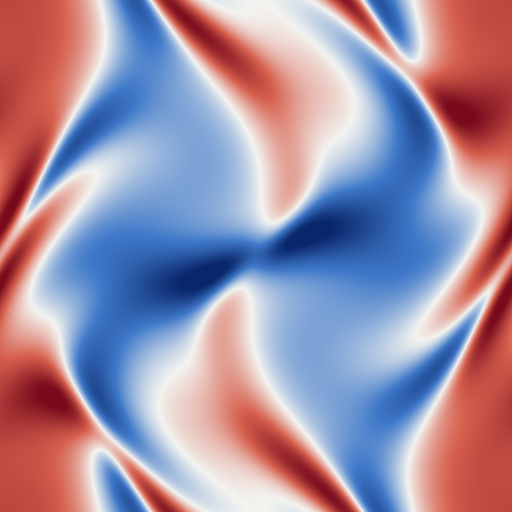
\includegraphics[width=0.40\textwidth]{ot_zeta_t05.png} &
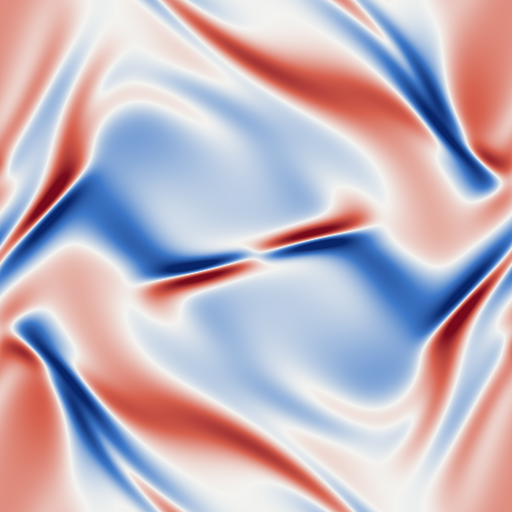
\includegraphics[width=0.40\textwidth]{ot_zeta_t1.png} \\[1mm]
{\small (a) vorticity $\zeta$, $t=0.5$\,s} & {\small (b) vorticity $\zeta$, $t=1$\,s} \\[3mm]
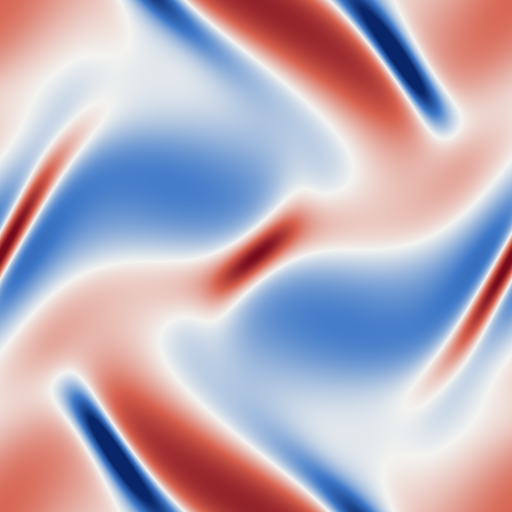
\includegraphics[width=0.40\textwidth]{ot_j_t05.png} &
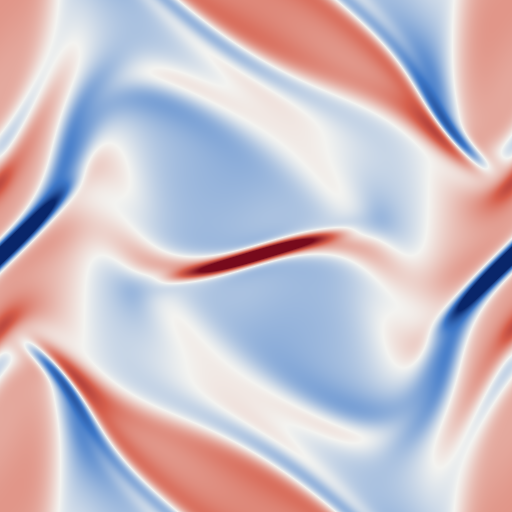
\includegraphics[width=0.40\textwidth]{ot_j_t1.png} \\[1mm]
{\small (c) current $j$, $t=0.5$\,s} & {\small (d) current $j$, $t=1$\,s} \\
\end{tabular}
\caption{Orszag--Tang vortex at $\mathrm{Re}\approx628$, $\mathrm{Pr}_m=1$, on a
$512^2$ grid with the hybrid central-moment operator. Diverging colour scale,
blue negative, red positive. The scale \emph{saturates at the 99th percentile of
$|v|$} --- $6.16$ and $11.13$ for $\zeta$, $12.88$ and $22.67$ for $j$ --- because
the current sheets are strongly localised: at $t=1$ the peak $|j|$ is $46.4$
against a 99th percentile of $22.7$, so scaling by the maximum would leave the
whole field pale. Between $t=0.5$ and $t=1$ the smooth initial vortex steepens
into the thin diagonal current sheet visible in panel (d), which is the feature
this benchmark exists to resolve and the reason $j_{\max}$ is the more
grid-sensitive of the two reported peaks.}
\label{fig:ot}
\end{figure}

\subsubsection{Comparison with published data}

Reproducing the setup of \cite{derosis2018}: $L=2\pi$\,m, $u_0=b_0=2$,
$\rho=1$\,kg\,m$^{-3}$, $N=1024$, $\Delta t=5\times10^{-5}$\,s. The derived lattice
parameters reproduce the published values exactly
($u_{0,\rm lat}=1.6297\times10^{-2}$, $\mathrm{Ma}=0.0282$), with
$\mathrm{Re}=u_0N/\nu$ in lattice units and $\mathrm{Pr}_m=1$. The reference
column is the high-resolution pseudo-spectral data quoted there.

\begin{center}\small
\begin{tabular}{llcccc}
\toprule
 & $t$ (s) & spectral & published LB & here, BGK & here, hybrid CM \\
\midrule
$j_{\max}$    & 0.5 & 18.24 & 18.24 & 18.23 & 18.23 \\
$j_{\max}$    & 1.0 & 46.59 & 46.65 & 46.55 & 46.55 \\
$\zeta_{\max}$& 0.5 & 6.758 & 6.756 & 6.756 & \textbf{6.756} \\
$\zeta_{\max}$& 1.0 & 14.20 & 14.18 & 14.182 & \textbf{14.180} \\
\bottomrule
\end{tabular}
\end{center}

\noindent Errors against the spectral reference are
$0.07 / 0.09 / 0.03 / 0.14\,\%$, where the published LB errors are
$0 / 0.13 / 0.03 / 0.14\,\%$: the same accuracy from an independent
implementation, with the hybrid scheme landing on the published vorticity values
to every quoted digit. Convergence toward the reference is second order, $j_{\max}$
at $t=1$ going $-1.92\%$ ($N=256$), $-0.46\%$ ($N=512$), $-0.09\%$ ($N=1024$).

The one residual is $j_{\max}$ at $t=1$, $0.22\%$ below the published value. That
is the quantity in which to expect it: the reference computes the current locally
from the distributions whereas this code uses second-order central differences,
and $j$ is the more gradient-sensitive of the two peaks. Vorticity agreeing
exactly while the current is $0.2\%$ low points at the derivative operator rather
than at the scheme.

\subsubsection{Stability at high Reynolds number}

At $\mathrm{Re}=5000$ the lattice viscosity gives $\tau=0.510$ on the $1024^2$
grid, close enough to $1/2$ that the BGK ghost modes go unstable. Runs are
terminated at the first non-finite field or at $\mathrm{Ma}>0.5$.

\begin{center}\small
\begin{tabular}{lccccc}
\toprule
grid & $\tau$ & BGK & hybrid CM & published BGK \\
\midrule
$512^2$  & 0.505 & blow-up $t=0.38$\,s & stable to $t=1.00$\,s & --- \\
$1024^2$ & 0.510 & blow-up $\bm{t=0.54}$\,s & stable to $\bm{t=1.20}$\,s & $t\approx0.52$\,s \\
\bottomrule
\end{tabular}
\end{center}

The BGK failure reproduces the published behaviour quantitatively --- within one
probe interval ($0.02$\,s) --- and shows the correct resolution dependence. Its
signature is instructive: $j_{\max}$ grows smoothly to $24.0$ at $t=0.50$, triples
to $73.7$ at $t=0.52$, then overflows, while the Mach number is $0.055$ at the
last clean sample. This is a collision instability, not a gradual compressibility
breakdown.

The hybrid central-moment scheme runs $2.2\times$ longer on the same grid and
passes the $t\approx0.99$\,s mark that defeated BGK even on a finer grid in
\cite{derosis2018}. Its $j_{\max}$ peaks at $166.2$ near $t=1.00$ and then
\emph{decays} smoothly to $155.4$ by $t=1.18$, with the Mach number bounded at
$0.069$ throughout. That turnover is the clearest evidence the run is genuinely
resolved rather than merely not-yet-diverged: an unstable run grows
monotonically, it does not turn over.

\subsubsection{Quasi-two-dimensional reduction: 3D lattices with $n_z=1$}
\label{sec:reduction}

The Orszag--Tang vortex is a two-dimensional problem, so running it on a 3D
lattice with a \emph{single} cell in $z$ is a reduction test: with $n_z=1$ and
periodic $z$ the neighbour wrap sends the out-of-plane neighbour back to the node
itself, the corresponding populations stream in place, and the answer must agree
with the native 2D lattice. No code change was required --- the wrap of
\S\ref{sec:periodic} and the pair swap of Table~\ref{tab:esopull} handle it.

The magnetic field follows the fluid's dimensionality by default (D2Q5 beside
D2Q9, D3Q7 beside D3Q27), but since $b_z\equiv0$ for this flow a 2D
magnetic lattice is a legitimate pairing and isolates its contribution.
Error against the spectral reference, per cent:

\begin{center}\small
\begin{tabular}{llcccc}
\toprule
fluid & magnetic & $j_{\max}(0.5)$ & $j_{\max}(1)$ & $\zeta_{\max}(0.5)$ & $\zeta_{\max}(1)$ \\
\midrule
\multicolumn{6}{l}{\emph{$N=256$}}\\
D2Q9  & D2Q5 & $-0.89$ & $-1.92$ & $-0.25$ & $-1.57$ \\
\textbf{D3Q27} & \textbf{D2Q5} & $\bm{-0.89}$ & $\bm{-1.92}$ & $\bm{-0.25}$ & $\bm{-1.57}$ \\
D3Q27 & D3Q7 & $-0.77$ & $-1.66$ & $-0.24$ & $-1.51$ \\
\midrule
\multicolumn{6}{l}{\emph{$N=512$}}\\
D2Q9  & D2Q5 & $-0.25$ & $-0.46$ & $-0.07$ & $-0.48$ \\
D3Q27 & D3Q7 & $-0.22$ & $-0.39$ & $-0.07$ & $-0.46$ \\
\bottomrule
\end{tabular}
\end{center}

Two results, one exact and one asymptotic.

\paragraph{D3Q27 reduces to D2Q9 exactly.} Not approximately: the agreement in
the highlighted row is structural, and both conditions for it can be checked in
exact arithmetic. First, summing the D3Q27 weights over $z$ reproduces the D2Q9
weights term for term,
\begin{equation}
  \tfrac{8}{27}+2\cdot\tfrac{2}{27} = \tfrac49, \qquad
  \tfrac{2}{27}+2\cdot\tfrac{1}{54} = \tfrac19, \qquad
  \tfrac{1}{54}+2\cdot\tfrac{1}{216} = \tfrac1{36},
\end{equation}
so for a $z$-invariant field the projected equilibrium and the projected BGK
update are exactly D2Q9's. Second --- and this is the part that is not automatic
--- the out-of-plane Maxwell-stress contribution cancels within every in-plane
group:
\begin{equation}
  \sum_{c_z} w_i\,\big(c_z^2-\cs^2\big) = 0
  \qquad\text{for each } (c_x,c_y) \ \text{on D3Q27}.
\end{equation}

\paragraph{The spread converges away.} Between $N=256$ and $N=512$ the
lattice-to-lattice spread falls from $0.12$, $0.26$ and $0.06$ percentage points
(on $j_{\max}(0.5)$, $j_{\max}(1)$, $\zeta_{\max}(1)$) to $0.03$, $0.07$ and
$0.02$ --- factors of $4.0$, $3.7$ and $3.0$, i.e.\ second order. The lattice
pairings are therefore converging to the same answer, and what separates them at finite
resolution is truncation error rather than different physics. Of the two
choices, the magnetic lattice matters more than the fluid one: swapping D2Q5 for
D3Q7 moves $j_{\max}$ by about $0.25$ percentage points at $N=256$, which is
unsurprising given $\cs^2=1/3$ against $1/4$ and correspondingly different
truncation in the induction equation.

%------------------------------------------------------------------------------
\subsection{Boundary conditions}
\label{sec:bcvalid}

Four tests, one per claim. All are second order, which is the accuracy of the
scheme itself, so what distinguishes the conditions is \emph{where the wall is},
and that is what each table measures rather than assumes.

\paragraph{Regularised walls: order and wall placement.} Poiseuille flow with
regularised walls on the boundary rows, $\tau=0.8$. The wall position is obtained
by fitting a parabola to the three interior nodes nearest the wall and taking its
root; reading $\uu$ back at the wall node would test nothing, since the solver
reports the imposed value there by construction.
\begin{center}\small
\begin{tabular}{rlll}
\toprule
$W$ & $L_2$ error & order & fitted wall position \\
\midrule
8  & $1.708\e{-2}$ & ---   & $2.68\e{-2}$ \\
16 & $4.419\e{-3}$ & 1.950 & $1.33\e{-2}$ \\
32 & $1.123\e{-3}$ & 1.976 & $6.67\e{-3}$ \\
\bottomrule
\end{tabular}
\end{center}
\noindent The offset halves with each refinement: first order in lattice units,
hence second order relative to the channel width. It is entirely the curvature
slip \eqref{eq:curvslip}: at $\tau=0.8$, $\frac43(\omega-1)/\omega^2 = 0.2133$
against $0.2128$ measured. At $\tau=1$ the same run is exact to $1\e{-15}$.

\emph{These numbers are worse than they were before the force corrections of
\S\ref{sec:regularized} were applied}, and that is worth stating rather than
hiding: without them the offset at $\tau=0.8$ was $1.42\e{-2}$, because the
force defect and the curvature slip carry opposite signs there and partially
cancelled. Two errors cancelling is not accuracy, and removing the one that is
understood is the right move even though a headline number rises. The order of
convergence is unchanged. D2Q9 and D3Q27 agree to
seven significant figures on this flow, the plane channel being quasi-one
dimensional so that D3Q27 with periodic span reduces exactly.

\paragraph{Corners: the two closures compared.} Lid-driven cavity, $129^2$,
against Ghia, Ghia and Shin~\cite{ghia1982}.
\begin{center}\small
\begin{tabular}{llll}
\toprule
$Re$ & corner closure & $\max|\Delta u|$ & $\max|\Delta v|$ \\
\midrule
100  & local        & 0.0044 & 0.0071 \\
100  & finite diff. & 0.0046 & 0.0065 \\
1000 & local        & 0.0187 & 0.0149 \\
1000 & finite diff. & \textbf{0.0123} & \textbf{0.0117} \\
\bottomrule
\end{tabular}
\end{center}
\noindent At $Re=100$ the two are indistinguishable --- four corner nodes out of
$16\,641$ do not move the centrelines. At $Re=1000$ the finite-difference closure
is better at \emph{every} station of the $u$ profile, by roughly a third in both
the maximum and the rms. The improvement sits in the near-wall regions and
vanishes in the core, which is the expected signature: the corner closure
perturbs the boundary layers, and at $Re=1000$ those are thin enough for the
perturbation to reach the centreline. This is why the finite-difference route is
the default.

\paragraph{Magnetic walls: Hartmann flow.} The MHD analogue of Poiseuille flow,
$\mathrm{Ha}=10$, $\nu=\eta$, against the exact solution~\cite{dellar2013bc}
\begin{equation}
  b(\xi) = \frac{FL}{B_0}\left[\frac{\sinh(H\xi)}{\sinh H}-\xi\right],
  \qquad
  u(\xi) = \frac{FL}{B_0}\sqrt{\frac{\eta}{\nu}}\coth H
           \left[1-\frac{\cosh(H\xi)}{\cosh H}\right],
  \label{eq:hartmann}
\end{equation}
with $\xi=x/L$ and $H=B_0L/\sqrt{\nu\eta}$. Velocity uses regularised walls,
$\bb$ uses the moment condition \eqref{eq:dellar13}; both put the wall on the
node, so they agree about where it is.
\begin{center}\small
\begin{tabular}{rllllll}
\toprule
$n$ & $\ell_2(u)$ & order & $\ell_2(b)$ & order & $|u|$ wall & $|b|$ wall \\
\midrule
17  & $3.873\e{-4}$ & ---   & $4.117\e{-4}$ & ---   & $0$ & $0$ \\
33  & $8.831\e{-5}$ & 2.133 & $1.009\e{-4}$ & 2.029 & $0$ & $0$ \\
65  & $2.136\e{-5}$ & 2.047 & $2.544\e{-5}$ & 1.988 & $0$ & $0$ \\
129 & $5.476\e{-6}$ & 1.964 & $6.572\e{-6}$ & 1.953 & $0$ & $0$ \\
\bottomrule
\end{tabular}
\end{center}
\noindent Second order in both fields, and both vanish at the walls exactly
rather than to $O(h^2)$ --- the property the moment condition exists to provide.
The computed profile reproduces the flat Hartmann core, the $O(L/H)$ boundary
layers, and $b(0)=1.1\e{-17}$, antisymmetry at round-off.

\paragraph{Inlet-driven Hartmann flow: the same problem without a body force.}
\label{sec:hartmanninlet}
The test above drives the channel with a uniform force through a
streamwise-periodic domain. Removing the force and driving it from an inlet
instead changes what is being tested in three ways, and each is the reason for
doing it:
\begin{itemize}[leftmargin=1.4em,itemsep=2pt]
\item It is the only way to put \code{MhdCentralMoments} against an analytic
      profile at all. That operator hardcodes \code{NoForcing} and cannot be
      body-force driven, so the force-driven test covers \code{MhdBGK} and could
      never have covered it.
\item It is free of the Guo half-force interaction and the curvature slip
      \eqref{eq:curvslip}, exactly as the inlet Poiseuille of
      \S\ref{sec:poisinlet} is.
\item It is the only test in the suite exercising the fluid and magnetic outflow
      conditions at once.
\end{itemize}

\noindent Dellar's axes are rotated so the streamwise direction is $x$: walls on
the two $y$-normal planes, half-width $L=(L_y-1)/2$, $\xi=(y-L)/L$, and the
applied field $B_0$ wall-normal along $y$, stretched by the flow into a
streamwise $b_x$. The exact solution is \eqref{eq:hartmann} with $x$ and $y$
interchanged. The velocity inlet imposes the analytic $u$, the outlet is the
constant back-pressure condition of \S\ref{sec:outflow}, and $\bb$ is imposed at
the inlet but left free at the outlet --- pinning it at both ends would tell the
induction equation the answer at both boundaries and make the interior test
partly circular.

\begin{center}\small
\begin{tabular}{rllllll}
\toprule
$L_y$ & rel $L_2(u)$ & order & rel $L_2(b)$ & order & $|u|$ wall & $|b|$ wall \\
\midrule
17  & $2.281\e{-2}$ & ---   & $6.499\e{-2}$ & ---   & $0$ & $0$ \\
33  & $5.391\e{-3}$ & 2.081 & $1.590\e{-2}$ & 2.031 & $0$ & $0$ \\
65  & $1.286\e{-3}$ & 2.068 & $3.916\e{-3}$ & 2.022 & $0$ & $0$ \\
129 & $3.071\e{-4}$ & 2.066 & $9.793\e{-4}$ & 2.000 & $0$ & $0$ \\
\bottomrule
\end{tabular}
\end{center}
\noindent $\mathrm{Ha}=10$, $\nu=\eta=0.1$, $u_{\max}=0.005$, $L_x=241$,
$L_z=1$. Second order in both fields, and both vanish at the wall node exactly.
The Hartmann profile has a flat core with layers of thickness $L/\mathrm{Ha}$, a
tenth of the channel here, so this is a considerably harder test of the wall
region than the parabolic Poiseuille profile.

\emph{Why $L_x$ is so large.} Not for physics: the magnetic outflow condition
contaminates a long stretch upstream, as \S\ref{sec:momentbc} records. With the
$L_x=21$ that the Poiseuille case uses, the contamination covers the entire
domain and the measured order is meaningless. The Mach floor of
\S\ref{sec:poisinlet} appears here too but is the smaller effect: at
$u_{\max}=0.02$ the last rate in $u$ falls to $1.461$, and dropping to
$u_{\max}=0.005$ recovers it.

\paragraph{Scalar walls: placement, measured.} Steady one-dimensional conduction
between walls at $T=0$ and $T=1$. The profile is exactly linear, so the residual
is round-off ($\sim10^{-14}$ throughout) and the only meaningful measurement is
where a least-squares line through the \emph{interior} nodes reaches the wall
values.
\begin{center}\small
\begin{tabular}{rllll}
\toprule
& \multicolumn{2}{c}{anti-bounce-back} & \multicolumn{2}{c}{moment condition} \\
\cmidrule(lr){2-3}\cmidrule(lr){4-5}
$N$ & $T=0$ at & $T=1$ at & $T=0$ at & $T=1$ at \\
\midrule
9  & 0.500000 & 7.500000  & $-0.000000$ & 8.000000  \\
17 & 0.500000 & 15.500000 & $-0.000000$ & 16.000000 \\
33 & 0.500000 & 31.500000 & $-0.000000$ & 32.000000 \\
65 & 0.500000 & 63.500000 & $-0.000000$ & 64.000000 \\
\bottomrule
\end{tabular}
\end{center}
\noindent Anti-bounce-back places its wall half a spacing outside the node, the
moment condition exactly on it, at every resolution and to machine precision.

%==============================================================================
\section{Validation campaign}
\label{sec:campaign}

The tests of \S\ref{sec:validation} were written alongside the features they
exercise. This section is different: it works through a published test suite
without modification, so that the numbers can be put beside someone else's.

The suite is Sec.~III of De Rosis and Coreixas~\cite{derosis2020}, tests III.A
to III.E, plus the inlet-driven Poiseuille flow of Sec.~III.A of De
Rosis~\cite{derosis2017pre}. Test III.F is out of scope: the campaign was
specified to exclude applied body forces, and III.F has one.

\paragraph{Settings, and where they depart from the papers.} Everything runs on
the central-moments operator with the highest-order equilibrium each lattice
admits (\S\ref{sec:eqsummary}) --- sixth order on D2Q9 and D3Q27. BGK and MRT
were deliberately not run. The two-dimensional cases are run on D2Q9 and on
D3Q27 with a single periodic point in $z$; III.E is genuinely
three-dimensional and uses D3Q27. Fixed $u_0=0.02$
throughout rather than the papers' sweeps, and reduced resolutions where cost
demanded: $D=64$ rather than $128$ in III.E, $D_{\rm lb}=512$ only in III.D,
$N=129$ rather than $201$ in III.C. These are stated per test below because in
two cases they change what the number means.

%------------------------------------------------------------------------------
\subsection{Taylor--Green vortex}

Periodic square of side $2\pi$, $N^2$ points, $\mathrm{Re}=1000$, error measured
at $t=T$ against the exact decaying solution.

\begin{center}\small
\begin{tabular}{lcccccc}
\toprule
$N$ & 8 & 16 & 32 & 64 & 128 & 256 \\
\midrule
D2Q9  & $1.106\e{-1}$ & $2.566\e{-2}$ & $6.259\e{-3}$ & $1.444\e{-3}$ & $2.427\e{-4}$ & $6.010\e{-5}$ \\
D3Q27 & $1.106\e{-1}$ & $2.566\e{-2}$ & $6.259\e{-3}$ & $1.444\e{-3}$ & $2.427\e{-4}$ & $6.010\e{-5}$ \\
\bottomrule
\end{tabular}
\end{center}
\noindent Fitted rate $2.186$ on both lattices. The paper
reports an optimal rate of $2$ at its lowest $u_0$.

\paragraph{A correction to the published initial condition.} Reference
\cite{derosis2020} prints
\begin{equation*}
  \uu_0 = u_0[\cos\gamma x\,\sin\gamma y,\;\sin\gamma x\,\cos\gamma y,\;0],
\end{equation*}
whose divergence is $-2u_0\gamma\sin\gamma x\sin\gamma y \neq 0$. Almost certainly a lost minus
sign in typesetting; the standard solenoidal field, with $-\cos\gamma x
\sin\gamma y$ in the first component, is used here. The printed density
likewise carries a leading factor $3$ that would give $\rho\approx 3$, and the
standard form is used instead.

%------------------------------------------------------------------------------
\subsection{Double shear layer}

$L=256$, $\mathrm{Re}=30\,000$, $\tau=0.500512$ --- a stability test rather than
an accuracy one, run to $t/t_0=1$. All three lattices complete without
divergence at that $\tau$, and the normalised invariants agree closely:

\begin{center}\small
\begin{tabular}{lcc}
\toprule
 & $E/E_0$ & $\Psi/\Psi_0$ \\
\midrule
D2Q9  & 0.986436 & 0.622701 \\
D3Q27 & 0.986436 & 0.622701 \\
\bottomrule
\end{tabular}
\end{center}

%------------------------------------------------------------------------------
\subsection{Lid-driven cavity}

$129^2$, $u_{\rm lid}=0.02$, against Ghia, Ghia and Shin~\cite{ghia1982}.
Reported as the largest absolute deviation over the 17 tabulated stations, in
lid-velocity units.

\begin{center}\small
\begin{tabular}{lcccccc}
\toprule
 & \multicolumn{2}{c}{$\mathrm{Re}=100$} & \multicolumn{2}{c}{$\mathrm{Re}=400$}
 & \multicolumn{2}{c}{$\mathrm{Re}=1000$} \\
\cmidrule(lr){2-3}\cmidrule(lr){4-5}\cmidrule(lr){6-7}
 & $\max|\Delta u|$ & $\max|\Delta v|$ & $\max|\Delta u|$ & $\max|\Delta v|$
 & $\max|\Delta u|$ & $\max|\Delta v|$ \\
\midrule
D2Q9  & 0.0049 & 0.0067 & 0.0069 & 0.0071$^\ast$ & 0.0094 & 0.0099 \\
D3Q27 & 0.0049 & 0.0067 & 0.0069 & 0.0071$^\ast$ & 0.0094 & 0.0099 \\
\bottomrule
\end{tabular}
\end{center}

\noindent $^\ast$\,\emph{One published reference value is anomalous, and it is
Ghia's, not a transcription error here.} All three tables in
\code{validation/cavity\_cm.cpp} have been checked entry-for-entry against an
independent digitisation of \cite{ghia1982} and they match. But the $v$ entry at
$\mathrm{Re}=400$, $x = 0.9063$ reads $-0.23827$, and three things say it cannot
be right:

\begin{itemize}\itemsep1pt
\item Ghia's own extremum table gives $\min v = -0.44993$ at $x = 0.8594$ for
      this Reynolds number. The three tabulated neighbours are then $-0.44993$
      $(0.8594)$, $-0.23827$ $(0.9063)$, $-0.22847$ $(0.9453)$: essentially the
      whole recovery from the minimum happens in one interval, after which the
      profile is flat.
\item The same three stations are smooth at $\mathrm{Re}=100$ ($-0.22445$,
      $-0.16914$, $-0.10313$) and at $\mathrm{Re}=1000$ ($-0.42665$, $-0.51550$,
      $-0.39188$). Only $\mathrm{Re}=400$ kinks, and at exactly one point.
\item Every other station agrees here to $0.0071$ or better; this one disagrees
      by $0.1415$, a factor of twenty. The value computed here, $-0.37974$, is
      what a smooth profile through Ghia's own minimum would give.
\end{itemize}

\noindent The entry is left in the table --- it is what the paper prints, and
quietly substituting a number nobody published would be worse --- but it is
excluded from the headline score above and reported separately by the run. It
could not be checked against the original paper, which is not among the
references to hand. An earlier draft of this document blamed the discrepancy on
a faulty transcription on this side; that was wrong, and the correction is
recorded here rather than silently applied.

%------------------------------------------------------------------------------
\subsection{Dipole--wall collision}

$D_{\rm lb}=512$ (a $1025^2$ grid), walls regularised, corners on the
finite-difference closure --- the only test in the campaign where the corner
treatment matters, since III.A, III.B and III.E are periodic. Against Table II
of \cite{derosis2020}, which reproduces the lattice Boltzmann results of
Mohammed, Graham and Reis~\cite{mohammed2018} and the spectral reference of
Clercx and Bruneau~\cite{clercx2006}:

\begin{center}\small
\begin{tabular}{clccc|ccc}
\toprule
 & & \multicolumn{3}{c|}{energy $E$} & \multicolumn{3}{c}{enstrophy $\Psi$} \\
$\mathrm{Re}$ & $t$ & here & \cite{mohammed2018} & \cite{clercx2006}
              & here & \cite{mohammed2018} & \cite{clercx2006} \\
\midrule
     & 0.25 & 1.4976 & 1.494 & 1.501 & 466.3 & 467.2 & 472.1 \\
625  & 0.5  & 1.0167 & 1.010 & 1.013 & 387.2 & 374.0 & 382.6 \\
     & 0.75 & 0.7702 & 0.765 & 0.767 & 251.3 & 244.8 & 256.0 \\
\midrule
     & 0.25 & 1.8355 & 1.838 & 1.848 & 689.6 & 705.3 & 725.6 \\
2500 & 0.5  & 1.5379 & 1.534 & 1.540 & 889.1 & 898.1 & 917.6 \\
     & 0.75 & 1.3274 & 1.320 & 1.325 & 790.3 & 790.2 & 809.9 \\
\bottomrule
\end{tabular}
\end{center}

\noindent Energy agrees to between $0.1\%$ and $0.7\%$ everywhere. Enstrophy is
the more demanding invariant and the agreement is between $0.01\%$ and $3.5\%$;
in most rows the value computed here falls \emph{between} the published lattice
Boltzmann result and the spectral one, and at $\mathrm{Re}=2500$, $t=0.75$ it
matches the published lattice Boltzmann enstrophy to four significant figures
($790.3$ against $790.2$). D2Q9 and D3Q27 are identical to every digit shown.

\paragraph{An error of ours, and how it was caught.} The published initial
condition is written in physical units with $|\omega_e| = 299.56$, which makes
$E(0)=2$ and $\Psi(0)=800$ exactly. It was first scaled so that the \emph{peak}
speed was $u_0$, which is wrong: the Reynolds number is built on the rms
velocity, and for this field the peak-to-rms ratio is $11.019$. The nominal
Reynolds number and the elapsed physical time were both a factor eleven out, the
flow dissipated far too slowly, and the discrepancy grew with $t$ --- a
signature that pointed at the time scale rather than at the wall. Verifying
Eq.~(32) numerically ($E(0)=2.0004$, $\Psi(0)=799.96$, $U_{\rm rms}=1.0001$)
settled it. The results above are from the corrected normalisation.

%------------------------------------------------------------------------------
\subsection{Three-dimensional Taylor--Green vortex}

$D=64$, run to $t^\ast = t u_0/D = 10$. There is no exact solution; the
comparison is between lattices. At the campaign's fixed $u_0=0.02$ the Mach
number is $0.035$ rather than the paper's $0.2$--$0.6$, so a unit of physical
time costs up to seventeen times more steps than in the paper.

\begin{center}\small
\begin{tabular}{lcc}
\toprule
 & $\mathrm{Re}=1600$ & $\mathrm{Re}=30\,000$ \\
\midrule
D3Q27 & completes, $E/E_0=0.0145$ at $t^\ast=10$ & completes, $E/E_0=0.0399$ at $t^\ast=10$ \\
\bottomrule
\end{tabular}
\end{center}

\noindent At $\mathrm{Re}=30\,000$ and this Mach number $\tau=0.50026$. That
case was initially judged infeasible on the available hardware; the judgement
was wrong, and D3Q27 runs it to $t^\ast=10$ without difficulty.

%------------------------------------------------------------------------------
\subsection{Inlet-driven Poiseuille flow}
\label{sec:poisinlet}

Sec.~III.A of \cite{derosis2017pre}. Laminar flow along $x$; no-slip on the two
$y$-normal planes; the parabolic profile $u_x(0,y) = 4U_0\,(y/L_y)(1-y/L_y)$
with $U_0 = 0.005$ imposed at the west face; outflow opposite; $L_x = 21$;
$\mathrm{Re} = U_0 L_y/\nu = 10$; started from rest and run to steady state. The
error is the relative $L_2$ norm, Eq.~(15) there, between the analytic profile
--- which equals the inlet profile, the flow being fully developed --- and a
$y$-aligned cross section at mid-domain. $L_z=1$ rather than the paper's $21$;
the flow has no $z$ dependence and $z$ is periodic either way. The outflow is
the constant back-pressure condition of \S\ref{sec:outflow}.

This test is worth having precisely because it is driven by the inlet and not by
a body force, so it is free of both the Guo half-force interaction and the
curvature slip \eqref{eq:curvslip} that dominate the forced channel of
\S\ref{sec:poiseuille}.

\begin{center}\small
\begin{tabular}{lccccc|c}
\toprule
$L_y$ & 41 & 81 & 161 & 321 & 641 & fitted rate \\
\midrule
D2Q9  & $1.160\e{-3}$ & $3.251\e{-4}$ & $7.261\e{-5}$ & $1.558\e{-5}$ & $6.192\e{-6}$ & 1.964 \\
D3Q27 & $1.160\e{-3}$ & $3.251\e{-4}$ & $7.261\e{-5}$ & $1.558\e{-5}$ & $6.192\e{-6}$ & 1.964 \\
\bottomrule
\end{tabular}
\end{center}

\noindent Against the published $2.063$ that is $4.8\%$ low.
The shortfall is entirely in the last refinement, where the pairwise rate drops
from $2.231$ to $1.334$, and it is understood --- see below. It is worth noting
first that the paper states its error at the finest grid, $L_y = 1281$, is of
order $10^{-5}$; the error here at $L_y=641$ is $6.2\e{-6}$, already below that.

\paragraph{What limits the order --- three falsified hypotheses.} The outlet was
the obvious suspect, and it is not the cause.

\begin{enumerate}\itemsep2pt
\item \emph{Per-station error.} Breaking the error down by $x$ at $L_y=641$
      makes the outlet look guilty: against $L_y=161$ the inlet station
      converges at $1.99$ and the bulk minimum at $1.92$, both clean second
      order, while the outlet station converges at $0.70$.
\item \emph{Moving the outlet away does not help.} Repeating at $L_x=41$ and
      $L_x=81$ makes the last pairwise rate \emph{worse}, not better:
      $1.334 \to 0.885 \to 0.007$. At $L_x=81$ the error stops responding to
      refinement altogether --- $5.974\e{-6}$ at $L_y=321$ against
      $5.945\e{-6}$ at $L_y=641$.
\item \emph{A second-order outlet does not help.} Replacing the zero-gradient
      tangential extrapolation by a linear one (\S\ref{sec:outflow}) is worse on
      the coarse grids and indistinguishable on the finest.
\end{enumerate}

\noindent What it actually is: a non-refining, velocity-dependent error.
Sweeping $U_0$ at fixed $\mathrm{Re}=10$ moves the onset of the degradation, and
always toward \emph{coarser} grids as $U_0$ rises.

\begin{center}\small
\begin{tabular}{ccccccc}
\toprule
$U_0$ & $\mathrm{Ma}$ & fitted rate & \multicolumn{4}{c}{pairwise rates} \\
\midrule
0.0025 & 0.0043 & \textbf{2.067} & 1.720 & 2.026 & 2.205 & 2.263 \\
0.005  & 0.0087 & 1.964 & 1.868 & 2.182 & 2.231 & 1.334 \\
0.01   & 0.0173 & 1.523 & 2.091 & 2.179 & 0.974 & 0.812 \\
0.02   & 0.0346 & 0.844 & 2.097 & 0.150 & 0.644 & 0.947 \\
\bottomrule
\end{tabular}
\end{center}

\noindent At $U_0 = 0.0025$ the velocity-dependent term stays below the
discretisation error across the whole range and the fitted rate is $2.067$,
against the published $2.063$ --- agreement to $0.2\%$. The scheme is second
order; the shortfall at $U_0=0.005$ is an artefact of the test's Mach number,
not a defect of the wall or the outlet.

This is not a novel observation. Reference \cite{derosis2020} reports the same
behaviour on its own Taylor--Green convergence study --- ``for the lowest value
of $u_0$, an optimal convergence value equal to 2 is found. As $u_0$ increases,
the accuracy and convergence properties of the method deteriorate as well'' ---
and attributes it to the cubic aliasing defect $c_{i\zeta}^3 = c_{i\zeta}$,
which prevents the diagonal terms $u_\zeta^3$ from entering the third-order
equilibrium moments and can only be removed by explicit correction terms. The
paper on this Poiseuille case~\cite{derosis2017pre} instead asserts that
$U_0=0.005$ gives a Mach number ``sufficiently low to annihilate detrimental
compressibility effects''; at the accuracy reached here that assertion does not
hold, which is unsurprising given that the error here at $L_y=641$ is already
below the error there at $L_y=1281$.

Fitting $\varepsilon = A/L_y^2 + B$ to the two finest grids gives $B<0$ at
$U_0=0.0025$ --- no floor reached --- and $B = 3.1\e{-6}$, $9.2\e{-6}$,
$2.1\e{-5}$ at $U_0 = 0.005$, $0.01$, $0.02$. That is growth somewhere between
linear and quadratic in $U_0$, but a two-point extraction is far too noisy to
pin the exponent and none is claimed.

%------------------------------------------------------------------------------
\subsection{Orszag--Tang vortex in three dimensions}
\label{sec:ot3d}

Section III.D and Fig.~6 of \cite{derosis2017pre}, with the initial condition
from Mininni, Pouquet and Montgomery~\cite{mininni2006}, that paper's Ref.~[38].
Cubic periodic box of side $2\pi$ on $M^3$ points, $\delta=2\pi/M$:
\begin{align}
  \uu(\xx,0) &= v_0\left[-2\sin(\delta y),\; 2\sin(\delta x),\; 0\right], \\
  \bb(\xx,0) &= 0.8\,b_0\left[-2\sin(2\delta y)+\sin(\delta z),\;
                              2\sin(\delta x)+\sin(\delta z),\;
                              \sin(\delta x)+\sin(\delta y)\right].
\end{align}
Both are solenoidal: each component depends only on coordinates it is not
differentiated by, so every term of the divergence vanishes identically.
$\mathrm{Re}=100$ on the lattice definition $\mathrm{Re}=v_0M/\nu$, $\Pr_m=1$,
D3Q27 for the fluid and D3Q7 for the field, central moments throughout.

\paragraph{Three things the paper leaves open.} Stated here because they change
the numbers, not buried in the code.
\begin{itemize}[leftmargin=1.4em,itemsep=2pt]
\item \emph{A sign.} Equation~(28) as printed has $+2\sin(\delta y)$ in the first
      velocity component; Ref.~\cite{mininni2006} has $-2\sin y$, which is what
      is used here. Unlike the two-dimensional Taylor--Green case in the same
      paper, the divergence does \emph{not} discriminate --- both forms are
      solenoidal --- so this rests on the cited source rather than on a
      consistency check. It is a genuine ambiguity, not a demonstrated typo.
\item \emph{$v_0$.} The paper says only that ``the values of $v_0$ and $b_0$ lead
      to a Mach number, $\mathrm{Ma}\sim0.034$'', and that depends on which speed
      $\mathrm{Ma}$ is built on. Taken here on the peak initial speed
      $2\sqrt2\,v_0$, giving $v_0=6.94\e{-3}$.
\item \emph{$b_0$.} Not given; set to $v_0$, the usual equipartition choice.
\end{itemize}

\paragraph{What can be checked.} Figure~6 is a plot against a high-resolution
pseudospectral run and those values are not available numerically, so no
per-point comparison is possible. What the figure \emph{does} supply is its axes
--- panel (a) plots the volume-averaged kinetic energy $\Gamma$ normalised from
$1$, panel (b) runs from $5$ to $25$ in $J_{\max}$ --- and the text states that
``the current shows a maximum at about $t=1$''.

\begin{center}\small
\begin{tabular}{rccc}
\toprule
$M$ & $J_{\max}$ peak & at $t$ & $\Gamma(4)$ \\
\midrule
32  & 15.71 & 1.194 & 0.1240 \\
64  & 19.19 & 1.198 & 0.1356 \\
128 & 20.43 & 1.200 & 0.1374 \\
\bottomrule
\end{tabular}
\end{center}

\noindent Every check the figure permits comes out right. The peak time
converges to $t=1.200$ against the stated $t\approx1$; $J_{\max}$ reaches $20.4$
on the finest grid, inside the $5$--$25$ axis; $\Gamma$ falls from $1$ to
$0.137$, inside the $0$--$1$ axis; and the curves converge monotonically upward
with $M$, the finer grids resolving the current sheet better, which is the trend
the figure reports.

\begin{figure}[htbp]
\centering
\begin{tikzpicture}
\begin{axis}[width=7.4cm, height=6.0cm,
  xlabel={time}, ylabel={$J_{\max}$},
  xmin=0, xmax=4, ymin=0, ymax=22,
  grid=both, grid style={line width=.2pt, draw=gray!25},
  major grid style={line width=.3pt, draw=gray!45},
  tick label style={font=\scriptsize}, label style={font=\small},
  legend style={font=\scriptsize, cells={anchor=west}, draw=gray!50,
                at={(0.98,0.98)}, anchor=north east, fill=white},
  every axis plot/.append style={line width=0.9pt, mark size=1.6pt},
  title={\small (a) peak current}]
  \addplot[opBGK, mark=*]        table[x=t,y=j] {ot3d_M32.dat};
  \addplot[opMRT, mark=square*]  table[x=t,y=j] {ot3d_M64.dat};
  \addplot[opCM,  mark=diamond*] table[x=t,y=j] {ot3d_M128.dat};
  \addplot[black, dashed, line width=0.6pt, forget plot] coordinates {(1,0) (1,22)};
  \node[font=\scriptsize, anchor=west, text=gray!70!black]
    at (axis cs:1.08,2.4) {paper: max at $t\approx1$};
  \legend{$32^3$, $64^3$, $128^3$}
\end{axis}
\end{tikzpicture}\hfill
\begin{tikzpicture}
\begin{axis}[width=7.4cm, height=6.0cm,
  xlabel={time}, ylabel={$\Gamma(t)/\Gamma(0)$},
  xmin=0, xmax=4, ymin=0, ymax=1.05,
  grid=both, grid style={line width=.2pt, draw=gray!25},
  major grid style={line width=.3pt, draw=gray!45},
  tick label style={font=\scriptsize}, label style={font=\small},
  legend style={font=\scriptsize, cells={anchor=west}, draw=gray!50,
                at={(0.98,0.98)}, anchor=north east, fill=white},
  every axis plot/.append style={line width=0.9pt, mark size=1.6pt},
  title={\small (b) volume-averaged kinetic energy}]
  \addplot[opBGK, mark=*]        table[x=t,y=gamma] {ot3d_M32.dat};
  \addplot[opMRT, mark=square*]  table[x=t,y=gamma] {ot3d_M64.dat};
  \addplot[opCM,  mark=diamond*] table[x=t,y=gamma] {ot3d_M128.dat};
  \legend{$32^3$, $64^3$, $128^3$}
\end{axis}
\end{tikzpicture}
\caption{Three-dimensional Orszag--Tang vortex, D3Q27 with central moments, to
be read against Fig.~6 of \cite{derosis2017pre}. (a) The peak current magnitude
rises with resolution as the current sheet is resolved, and its maximum
converges to $t=1.200$ against the paper's stated $t\approx1$; the value on the
finest grid, $20.4$, sits inside that figure's $5$--$25$ axis. (b) The energy,
normalised as the paper normalises it, falls from $1$ to $0.137$. Both panels
use a linear time axis; the published figure uses a logarithmic one.}
\label{fig:ot3d}
\end{figure}

\paragraph{Convergence, and what it does and does not establish.} Equation~(30)
of \cite{derosis2017pre} defines $\chi$ as the $L_\infty$ norm of the relative
discrepancy against the spectral reference, quoted there as of order $10^{-2}$
for the finest grid. With no reference values to hand, the same measure is
computed against $M=128$ as a stand-in:
\begin{center}\small
\begin{tabular}{lcc}
\toprule
against $M=128$ & $\Gamma$ & $J_{\max}$ \\
\midrule
$M=32$ & $1.56\e{-2}$ & $2.31\e{-1}$ \\
$M=64$ & $1.9\e{-3}$  & $6.05\e{-2}$ \\
\bottomrule
\end{tabular}
\end{center}
\noindent The successive differences in the $J_{\max}$ peak are $0.171$ and
$0.061$, a ratio of $2.83$ --- close to second order on a quantity that is a
derivative of the field and therefore the hardest thing here to converge. The
$M=64$ figures, $6.1\e{-2}$ on $J_{\max}$ and $1.9\e{-3}$ on $\Gamma$, bracket
the $10^{-2}$ the paper quotes.

\emph{This is self-convergence, not agreement.} Substituting our own finest grid
for the spectral reference flatters systematically, because it cannot see any
error common to all three grids. It establishes that the scheme converges and
roughly how fast; it does not independently establish that it converges to the
right answer. Read the table above as a consistency check, not as a score.

\medskip
\noindent One incidental result worth recording: at $M=32$ this runs at
$\tau=0.507$, close enough to $1/2$ that BGK ghost modes are normally a problem,
and it completes the full $t\in[0,4]$ without difficulty --- consistent with the
stability advantage \cite{derosis2017pre} claims for central moments.

%------------------------------------------------------------------------------
\subsection{A finding that cuts across the campaign}

\paragraph{D2Q9 and D3Q27 with one point in $z$ are bit-identical.} Not merely
close: identical to every digit printed, in the Taylor--Green convergence, the
shear layer, the dipole, the cavity and the inlet Poiseuille --- five
independent tests. The reduction of D3Q27 to D2Q9 under a single periodic $z$
point is exact, which is a useful correctness check in both directions: it
exercises the 3D code path against the 2D one on every one of these flows.

%------------------------------------------------------------------------------
\subsection{Field snapshots}
\label{sec:snapshots}

The tables elsewhere in this section say whether a number is right. These say
whether the \emph{flow} is right, which is a different question and one a norm
cannot answer: a scheme can hit an integral quantity while getting the structure
wrong. Every panel below is the field the corresponding test actually converged
to, dumped from the run that produced the numbers quoted for it.

Signed quantities --- vorticity, current --- use a diverging map centred on
zero; quantities with no meaningful zero --- temperature, speed --- use a
sequential one. Where the colour saturates below the peak, the caption says so:
these fields are strongly localised, and scaling by the maximum leaves the
structure that matters invisible.

\begin{figure}[htbp]
\centering
\begin{tabular}{cc}
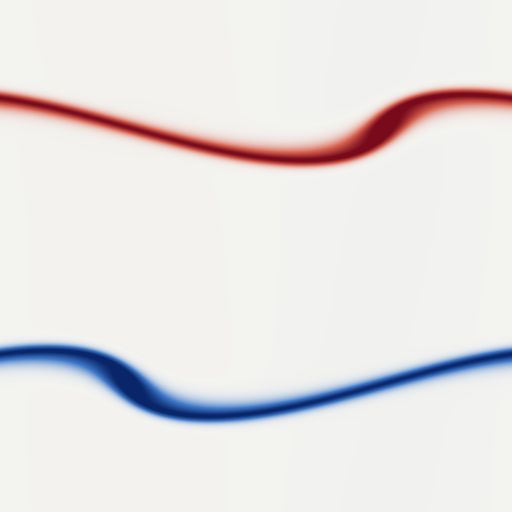
\includegraphics[width=0.40\textwidth]{sl_zeta_L512_t05.png} &
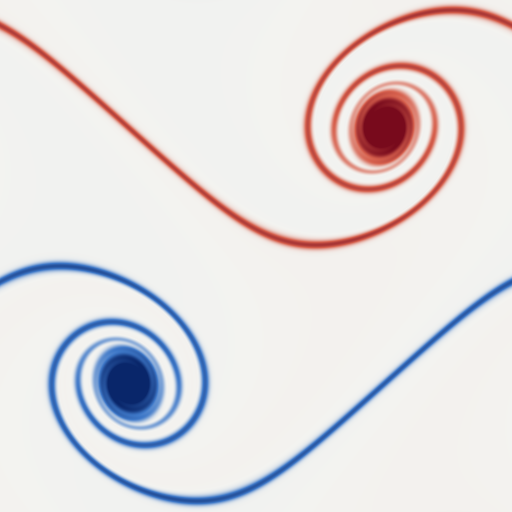
\includegraphics[width=0.40\textwidth]{sl_zeta_L512_t10.png} \\[1mm]
\small (a) $t/t_0 = 0.5$ & \small (b) $t/t_0 = 1$ \\
\end{tabular}
\caption{\textbf{Double shear layer}, vorticity, $L=512$,
$\mathrm{Re}=30\,000$, D2Q9 central moments (\S\ref{sec:campaign}). By (a) the
perturbation has begun to distort the two layers; by (b) each has rolled into a
vortex, and the two are joined by a single unbroken braid. That the braid stays
thin and connected is the whole test: at $\tau = 0.50102$ the flow is barely
resolved, and an under-dissipative or unstable scheme shows it here first, by
fragmenting the braid into secondary vortices that are numerical rather than
physical. Doubling the resolution from the $L=256$ of the campaign table sharpens the
structure and, more usefully, quantifies the numerical dissipation: the
enstrophy retained at $t/t_0=1$ rises from $0.6227$ to $0.6432$, and the energy
from $0.98644$ to $0.98696$. The physical dissipation at this Reynolds number is
negligible over one turnover, so nearly all of that difference is the scheme's
own, and it shrinks with resolution as it should. Colour saturates at the 99th
percentile of $|\zeta|$.}
\label{fig:shear}
\end{figure}

\begin{figure}[htbp]
\centering
\begin{tabular}{cc}
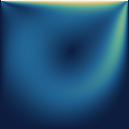
\includegraphics[width=0.34\textwidth]{cav_speed_re400.png} &
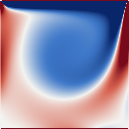
\includegraphics[width=0.34\textwidth]{cav_zeta_re400.png} \\[1mm]
\small (a) speed $|\uu|/u_{\rm lid}$ & \small (b) vorticity \\
\end{tabular}
\caption{\textbf{Lid-driven cavity} at $\mathrm{Re}=400$, $129^2$, D2Q9 central
moments, the run scored against Ghia \emph{et al.}\ in \S\ref{sec:campaign}
($\max|\Delta u| = 0.0069$). The primary vortex sits above and right of centre
and both downstream corner eddies are resolved. The vorticity is clipped hard,
at the 88th percentile against a peak twenty times larger, because it is
concentrated in the lid boundary layer; without that the interior is blank.}
\label{fig:cavity}
\end{figure}

\begin{figure}[htbp]
\centering
\begin{tabular}{cc}
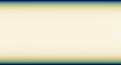
\includegraphics[width=0.40\textwidth]{hm_ux.png} &
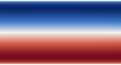
\includegraphics[width=0.40\textwidth]{hm_bx.png} \\[1mm]
\small (a) velocity $u_x$ & \small (b) induced field $b_x$ \\
\end{tabular}
\caption{\textbf{Inlet-driven Hartmann flow}, $\mathrm{Ha}=10$, $L_y=65$,
D2Q9 fluid with D2Q5 induction, central moments
(\S\ref{sec:hartmanninlet}). The velocity shows the flat Hartmann core with
boundary layers of thickness $L/\mathrm{Ha}$; the induced field is antisymmetric
about the centreline, vanishing there and at both walls. Both are visibly
independent of the streamwise coordinate, which is the property the exact
solution has and which the convergence table depends on --- any $x$ structure
here would be boundary error, and it is how the magnetic outflow defect
(\S\ref{sec:momentbc}) was found.}
\label{fig:hartmann}
\end{figure}

\begin{figure}[htbp]
\centering
\begin{tabular}{ccc}
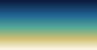
\includegraphics[width=0.30\textwidth]{rb_T_ra1500.png} &
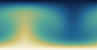
\includegraphics[width=0.30\textwidth]{rb_T_ra10000.png} &
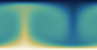
\includegraphics[width=0.30\textwidth]{rb_T_ra100000.png} \\[1mm]
\small (a) $\mathrm{Ra}=1500$ &
\small (b) $\mathrm{Ra}=10^{4}$ &
\small (c) $\mathrm{Ra}=10^{5}$ \\
\small $Nu = 1.0000$ & \small $Nu = 2.6490$ & \small $Nu = 4.9869$ \\
\end{tabular}
\caption{\textbf{Rayleigh--B\'enard convection}, temperature, $H=48$, one
critical wavelength wide, D2Q9 fluid with a D2Q5 scalar (\S\ref{sec:rbconv}).
The three panels are the same run at three Rayleigh numbers and show what the
Nusselt column of that section measures. (a) is \emph{below} the critical
$\mathrm{Ra}_c = 1707.762$: the perturbation decays and the field relaxes to
pure conduction --- a linear vertical gradient, no horizontal structure, and
$Nu = 1$ to $6\e{-13}$. (b) is supercritical, and the same perturbation grows
into a steady convection cell with a hot plume rising against cold fluid
descending. By (c), at $58.6\,\mathrm{Ra}_c$, the thermal boundary layers at the
two plates have thinned and the core is nearly isothermal --- which is the
mechanism behind $Nu$ rising to $4.99$, since $Nu$ is precisely the wall
gradient normalised by the conductive one. All three share a colour scale.}
\label{fig:rb}
\end{figure}

\begin{figure}[htbp]
\centering
\begin{tabular}{cc}
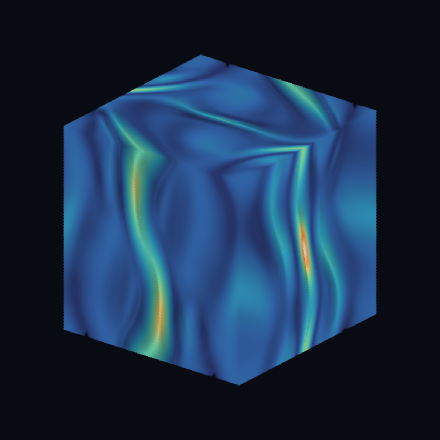
\includegraphics[width=0.40\textwidth]{ot3d_vol_t1.png} &
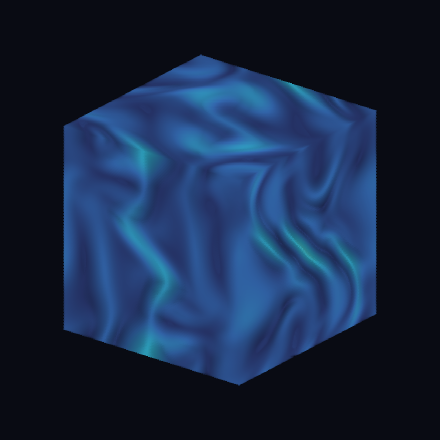
\includegraphics[width=0.40\textwidth]{ot3d_vol_t2.png} \\[1mm]
\small (a) $t = 1$, peak current & \small (b) $t = 2$ \\
\end{tabular}
\caption{\textbf{Three-dimensional Orszag--Tang vortex}, current magnitude
$|\nabla\times\bb|$ through the whole $128^3$ box, D3Q27 with D3Q7 induction
(\S\ref{sec:ot3d}). Volume rendered rather than sliced: a cut plane shows the
sheets only where they happen to intersect it and says nothing about how they
are oriented, which for this flow is the point. The current organises into
curved sheets wrapping the box, and (a) is the instant the peak is reached ---
the same $t\approx1$ the $J_{\max}$ curve of Fig.~\ref{fig:ot3d} locates.
\emph{Both panels share one colour scale}, set by the $t=1$ peak, so the visible
dimming from (a) to (b) is the real decay: $J_{\max}$ falls from $19.1$ to
$8.32$, less than half, in the same units as Fig.~\ref{fig:ot3d}. Normalising
each panel to its own maximum --- the default in most rendering tools --- would
have made the later, weaker field the brighter of the two. The reference is
recomputed at this resolution rather than carried over from the $64^3$ volumes:
the raw lattice values differ between the two by the factor $\Delta t \propto
1/M$ alone, so reusing the coarse-grid number would have rescaled the pair by
about two. Orthographic view, azimuth $38^\circ$, elevation
$24^\circ$; emission--absorption compositing with the weak field left
transparent, the local gradient used as a surface normal for a diffuse term so
the sheets read as surfaces rather than fog, and $2\times$ supersampling.
Rendered by \code{doc/fig/vol3d.py}, which is self-contained.}
\label{fig:ot3dfield}
\end{figure}

%==============================================================================
\section{Demonstrator: flow in a patient-specific aorta}
\label{sec:aorta}

Everything else in this document runs on a geometry described by a formula. This
one loads a voxel array off disk. It is included as a \emph{demonstrator}, not as
a validation case, and the distinction is worth stating precisely because the
figures are seductive: there is no analytic solution here, no reference data is
compared against, and \textbf{no number in this section is a claim of accuracy}.
What it demonstrates is that the solver runs unmodified on a geometry with no
symmetry and no closed form --- \code{set\_geometry} already takes an arbitrary
predicate, so real geometry needed a reader, not a new solver.

\subsection{Geometry and its verification}
\label{sec:aortageom}

\code{src/io/VoxelGeometry.hpp} reads the flat binary produced by voxelising a
SimVascular surface mesh (case \code{0074\_H\_AO\_H}): $109\times184\times361 =
7\,240\,216$ voxels at a pitch of $0.0616$\,cm, tagged $0$ solid, $1$ fluid,
$2$ inlet, $3$ outlet. Solid is $83.65\%$ of the box; the lumen is $16.31\%$.
The optional second inlet normal is detected by \emph{file size}, not by stream
state --- guessing from the stream would silently read 24 bytes of the tag array
as doubles on a file that does not carry one.

Three checks were run on the geometry before any flow was believed.

\begin{enumerate}[leftmargin=1.4em,itemsep=3pt]
\item \textbf{Connectivity.} A six-connected flood fill seeded from an inlet
  voxel reaches $1\,184\,057$ of $1\,184\,057$ non-solid voxels: one lumen, no
  isolated pockets. This check exists because a single constant-$x$ plane
  through this vessel cuts it into \emph{two} disconnected regions --- the aortic
  root and the arch --- which looks exactly like a hole in the mesh and is not
  one. The projected silhouette is a single connected region, as the flood fill
  requires it to be.

\item \textbf{Caps.} Under six-connectivity the inlet fragments into $303$ pieces
  and the outlets into $270$. This is not damage: an oblique plane on a voxel
  grid is diagonally connected, not face-connected. By centroid they are one
  inlet and four outlets --- three arch branches and the descending aorta.

\item \textbf{Domain edges.} $1283$ fluid voxels sit on the box boundary carrying
  no cap tag. Were the domain periodic these would wrap, connecting the
  descending aorta to the arch and corrupting the field silently. It is not:
  the case constructs \code{Domain(nx,ny,nz,false,false,false)}, and
  independently there are \emph{zero} fluid-to-fluid wrap pairs on any axis. The
  mesh is clipped flush against the box there and those voxels act as wall.
\end{enumerate}

\subsection{Boundary conditions}
\label{sec:aortabc}

\paragraph{The vessel wall} is halfway bounce-back on solid voxels, which under
Esoteric Pull costs nothing: bounce-back is the identity on the storage, so solid
cells are skipped outright --- no load, no store, no arithmetic
(\S\ref{sec:esopull}). The population a fluid node emits toward the wall sits
untouched for one step and is read back reversed on the next, placing the no-slip
surface midway between the last fluid node and the first solid node. Halo cells
are flagged \code{Excluded} and skipped by the same mechanism, so the box faces
behave identically.

\paragraph{The inlet} is a regularised velocity wall along the cap normal stored
in the file. The cap is oblique to the voxel axes, so it has no single face
normal; it is given \code{NrmCorner}, whose unknown set is built geometrically
per node rather than from an axis. Using a face normal instead would drive flow
into the wall.

\paragraph{The outlets} are left at fixed pressure rather than a prescribed flow
split, so the division of flow between the branch vessels is an \emph{output}
rather than an input. Imposing $\uu=0$ there would close the domain --- measured
as mass rising monotonically, $+8.5\e{-3}$ in 2000 steps.

\paragraph{Conserving outflow.} The outlet overwrites its nodes every step, so
whatever density is imposed is injected regardless of what arrived: pinning
$\rho=1$ makes the boundary a mass source and sink, and inlet and outlet fluxes
then differ by ${\sim}60\%$ with no way to tell which is wrong. Closing a loop on
\emph{total mass} instead makes it conserving --- raise the outlet density when
mass is lost, lower it when mass accumulates. The fixed point is the density at
which what leaves equals what enters, and it is found rather than assumed. Two
details are load-bearing. The error must be normalised by total mass, not by
outlet-node count: normalising by the latter gives an error of order $3$, which
saturates the clamp, reverses the flow and diverges the run in 1500 steps. And
the controller is held off until the vessel has filled, since during filling mass
\emph{should} be changing and the loop otherwise fights the physics.

Note that the finite-difference corner-stress path is disabled for this case. It
walks a two-node stencil off each wall node; in a box those neighbours are fluid
or wall, but in a vessel they are frequently \emph{solid}, whose populations
Esoteric Pull never updates, so the stencil reads stale memory and feeds garbage
stress into the inlet. The local closure is used instead until that path is made
geometry-aware.

\subsection{Steady inflow}
\label{sec:aortasteady}

$\mathrm{Re}=50$ on the inlet cap's equivalent diameter $D = 2\sqrt{A/\pi} =
32.9$ lattice units, $U=0.02$, $\nu=1.3167\e{-2}$, $\tau=0.5395$, D3Q27 central
moments. After $13\,500$ steps the run is steady: $|\uu|_{\max}$ flat at
$7.2\e{-2}$, outlet density settled at $0.9934$, and the mass error oscillating
about zero at ${\sim}1\e{-5}$ --- which is the conserving outflow working.

The inlet flux is $12.98$ in lattice units, and this is worth one sentence
because measuring it is less obvious than it looks. Summing over \emph{every}
exposed face of the cap gives $|\sum \nn_{\rm face}| = 653.2$ pointing within
$0.65^\circ$ of the normal stored in the file, so $U A\cos\theta = 0.02 \times
653.2 \times 0.9935 = 12.98$. Filtering the faces by direction to exclude the
vessel wall was tried and is \emph{wrong} --- it double-weights by the projection
and drove the figure down to $10.38$. The lateral wall faces already cancel in
the vector sum; that is what makes the identity $\sum\nn_{\rm face} = A\nn$ hold.

The outlet flux is \textbf{not} a valid measure for this boundary and is not used
as one: the condition overwrites populations, so a flux summed through it
reports the imposed state rather than what the flow delivered. Mass conservation
is the trustworthy check.

\subsection{Pulsatile inflow}
\label{sec:aortapulse}

The inlet is driven by the waveform used in the source project, reproduced
unchanged so the two are comparable:
\begin{equation}
  \frac{U(t)}{U_0} = \min\!\left(1,\frac{t}{t_{\rm ramp}}\right)
    \Big[0.15 + 0.85\,w(\phi)^{3/2}\Big],
  \qquad
  w(\phi) = \tfrac12 + \tfrac12\sin\!\Big(2\pi\phi - \tfrac{\pi}{2}\Big),
  \label{eq:aortawave}
\end{equation}
with $\phi = (t \bmod T)/T$: a ramp from rest, then a cycle between a diastolic
floor at $15\%$ of peak and a systolic peak, the upstroke sharpened by the $3/2$
power. $\phi=0$ is the diastolic minimum and the systolic peak falls at
$\phi=0.5$. Here $T=2000$, $t_{\rm ramp}=800$, and $U_0$ is the systolic peak.

Since the direction is fixed by the cap normal and only the magnitude varies, the
whole drive is a scale on the deduplicated wall-velocity table
(\code{set\_wall\_velocity\_scale}), not a per-node update, and costs nothing per
step. The scale multiplies a saved copy of the original table rather than the
live one: scaling in place would compound, and a waveform bounded in $[0,1]$
would become a product of its own history and decay to zero within a few hundred
steps --- which would look like a plausible physical relaxation and is not one.

The parameter that characterises a pulsatile flow is not $\mathrm{Re}$ but the
Womersley number, which fixes how far the oscillating shear layer penetrates in a
beat:
\begin{equation}
  \alpha = \frac{D}{2}\sqrt{\frac{2\pi}{T\nu}} = 8.04 ,
  \label{eq:womersley}
\end{equation}
in the physiological range for an aorta. The drive is exact beat after beat:
$Q_{\rm in}$ reaches $-12.98043$ at every systolic peak and $-1.947065$ at every
trough, identical to five digits across six cycles.

\paragraph{Convergence.} The viscous diffusion time across the vessel is
$R^2/\nu = 20\,552$ steps, which is $10.3$ beats. This run is $60\,000$ steps,
$2.92$ diffusion times, and it is converged: sampled at matched phase over the
final three beats, \emph{every} statistic of the speed field repeats to eight
significant figures.

\begin{center}\small
\begin{tabular}{clcccc}
\hline
$\phi$ & step & mean & median & $p_{99}$ & $|\uu|_{\max}$ \\
\hline
0.0 & 54000 & 0.00364663 & 0.00238384 & 0.0153191 & 0.0565515 \\
0.0 & 56000 & 0.00364663 & 0.00238384 & 0.0153191 & 0.0565515 \\
0.0 & 58000 & 0.00364663 & 0.00238384 & 0.0153191 & 0.0565515 \\
0.5 & 55000 & 0.00483408 & 0.00495437 & 0.0104059 & 0.0320153 \\
0.5 & 57000 & 0.00483408 & 0.00495437 & 0.0104059 & 0.0320153 \\
0.5 & 59000 & 0.00483408 & 0.00495437 & 0.0104059 & 0.0320153 \\
\hline
\end{tabular}
\end{center}

\noindent The residual differences are in the eighth digit, which is round-off.
The outlet density has stopped moving at $0.99699$, so the mass controller has
found its fixed point rather than still walking toward one. An earlier
$12\,800$-step run --- $0.62$ diffusion times --- was reported in a previous
draft of this section as \emph{not} converged, with mean and median still rising
monotonically through six beats. That was accurate, and it is what a run of that
length looks like; it is superseded rather than corrected.

\paragraph{Phase relationships, and a storage effect that is not Womersley.}
Over a converged beat the \emph{mean} speed peaks at $\phi=0.60$ against a drive
peaking at $\phi=0.50$: a lag of $0.10$ of a cycle, $36^\circ$, the expected
sense and order for $\alpha=8$.

The fast tail does the opposite. Both $p_{99}$ and $|\uu|_{\max}$ peak at
$\phi=0$ and reach their \emph{minimum} at systole --- nearly antiphase with the
drive. This is not a transient: it repeats identically across the final three
beats, and it is visible in Fig.~\ref{fig:aortapulse}, where at the diastolic
trough the root has gone pale while the descending aorta carries the fastest
flow in the vessel.

The mechanism is storage, not phase lag. Total mass is not constant over a beat:
it swings by $\pm2.7\e{-3}$, with its minimum at $\phi=0.25$ and its maximum at
$\phi=0.70$, accumulating through systole and discharging through diastole. The
fast tail peaks where that discharge is steepest. A transit-time explanation was
considered and does not survive arithmetic --- at these speeds a fluid particle
needs several beats to cross the vessel.

What this data does \emph{not} settle is where the storage lives. Two candidates
produce the same signature and are not distinguished by the dumps taken here,
which carry velocity but not density: the lattice fluid's own $O(\mathrm{Ma}^2)$
compressibility acting as a compliance chamber, or the fixed-pressure outlet
acting as a reservoir. Either way the effect is numerical rather than
physiological --- the wall is rigid (\S\ref{sec:aorta}, and the Known
Limitations) --- so the antiphase should not be quoted as a Womersley result,
and the fast tail should not be read as a haemodynamic observation.
$|\uu|_{\max}$ in particular is a single staircase-corner voxel and should not
be used at all.

\begin{figure}[htbp]
\centering
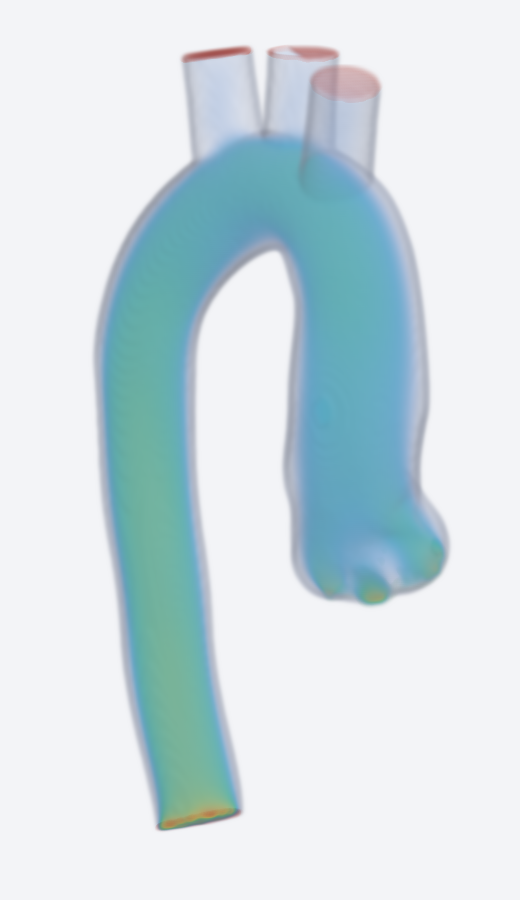
\includegraphics[width=0.32\textwidth]{aorta_steady.png}
\caption{\textbf{Steady inflow at $\mathrm{Re}=50$}, speed, after $13\,500$
steps. Volume rendering: a pale translucent shell wherever the lumen mask has a
gradient, diffuse-shaded off that gradient, with speed-coloured interior showing
through. Inlet cap green at the aortic root, outlet caps red. A single plane
through this vessel cuts it into disconnected islands, which is why the whole
volume is cast rather than sliced.}
\label{fig:aortasteady}
\end{figure}

\begin{figure}[htbp]
\centering
\begin{tabular}{cc}
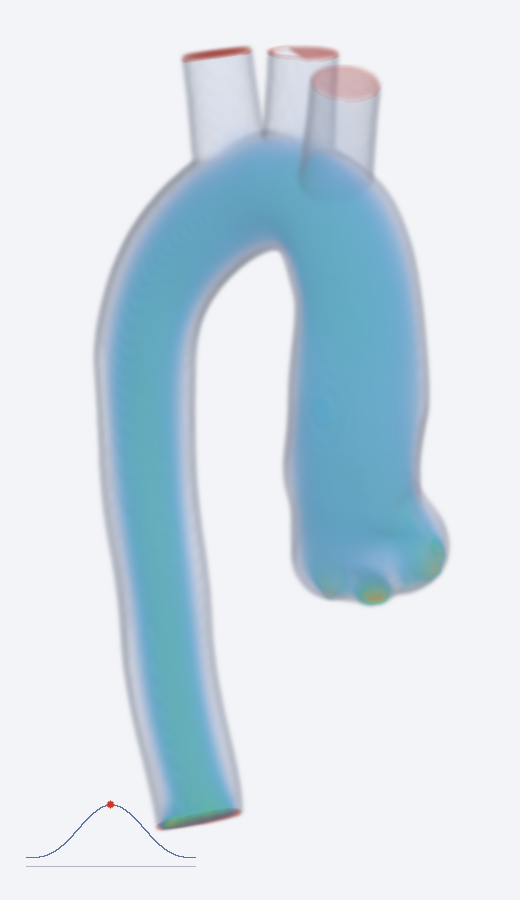
\includegraphics[width=0.32\textwidth]{aorta_systole.png} &
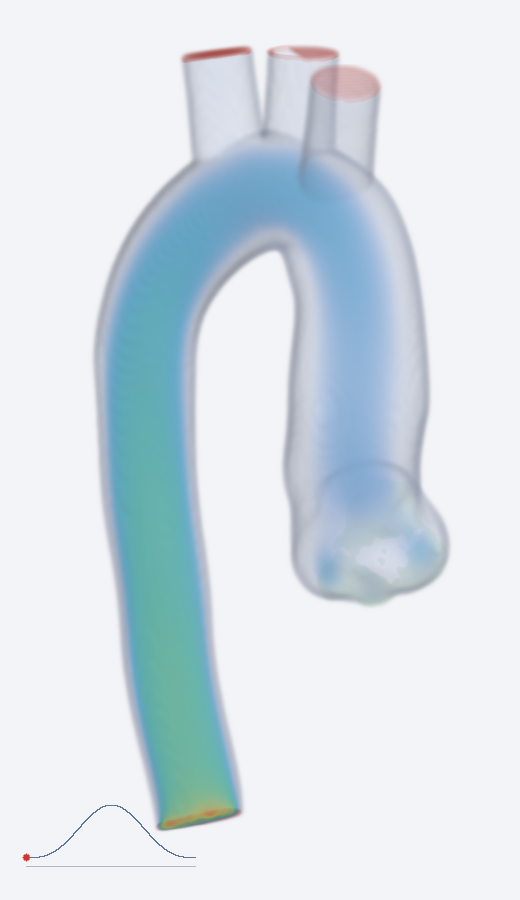
\includegraphics[width=0.32\textwidth]{aorta_diastole.png} \\[1mm]
\small (a) systolic peak, $\phi=0.5$ & \small (b) diastolic trough, $\phi=0$ \\
\end{tabular}
\caption{\textbf{Pulsatile inflow}, converged, $\alpha=8.04$, shared colour
scale, with streamlines traced from the inlet cap through the current field. The
inset traces \eqref{eq:aortawave} with a marker at the current phase. At systole
the root drives a visible jet; at the diastolic trough it has gone pale while the
descending aorta carries the fastest flow in the vessel --- the antiphase fast
tail of \S\ref{sec:aortapulse}, which is a storage-and-release effect and not a
Womersley lag. Both panels are from the same beat, at $2.9$ viscous diffusion
times, where every speed statistic repeats to eight significant figures from beat
to beat.}
\label{fig:aortapulse}
\end{figure}

%==============================================================================
\section{Demonstrator: urban pollutant dispersion}
\label{sec:urban}

The second demonstrator, and the second geometry source. A passive scalar is
released into a city and transported by an atmospheric wind over building
geometry read from a height field (\S\ref{sec:heightfield}). Like the aorta,
this is a demonstrator and not a validation case: there is no analytic solution
for a plume in a real city and no measurement to compare against, so nothing
here can fail except by crashing. What \emph{can} be checked is reported as a
number, and one of those numbers turned out to matter.

\subsection{Geometry from a height field}
\label{sec:heightfield}

Urban geometry does not arrive as a voxelised surface mesh. It arrives as
building footprints with heights, so the reader for it is a different one from
the aorta's (\S\ref{sec:aortageom}): a two-dimensional map of building height
in metres, plus a small JSON of grid metadata, with a cell solid when its centre
lies below the local height. That keeps $O(n_x n_y)$ on disk instead of
$O(n_x n_y n_z)$ --- for Manchester, $640$~kB rather than the $9.6$~million
cells it expands to.

Two decisions in that reader are about failure modes rather than features, and
both are there because \emph{none} of the ways it can go wrong produce an
error. A transposed index order rotates the city; a mis-parsed cell size
rescales it; an off-by-one in the solid rule shaves a layer off every roof. All
three run to completion and produce a plausible plume. So a missing key in the
metadata is an error rather than a default --- falling back to a built-in grid
size turns a typo into a silently wrong domain --- and a vertical spacing that
disagrees with the horizontal one is rejected rather than silently stretching
the city. The regression test compares against independently known values
throughout, using a deliberately asymmetric height pattern so that a transpose
changes what is read back.

On the real data the reader is checked against an independent implementation:
Manchester city centre, $400\times400\times60$ at $5$~m, $171\,375$ solid cells
of $9.6$~million ($1.79\%$), tallest column $200.5$~m --- matching cell for
cell.

\subsection{The model, and its principal limitation}

The wind is prescribed: a neutral-stability logarithmic surface layer
$u(z) = (u_*/\kappa)\ln((z+z_0)/z_0)$, horizontal, along a fixed compass
bearing, simply zeroed inside buildings. It has no street-canyon recirculation,
no building wake and no channelling along avenues --- which are precisely the
phenomena an urban dispersion study is about. The scalar side is the validated
one: D3Q7 transport, adiabatic buildings and ground, and the open boundaries of
\S\ref{sec:scalaroutflow}.

The time step follows from capping the fastest cell at a chosen lattice
velocity, and the relaxation rate then follows from the physical diffusivity.
Deriving $\Delta t$ from the wind and $\omega$ from $\Delta t$, rather than
choosing $\tau$ and letting $\Delta t$ fall out, is what keeps the advective
Courant number bounded --- the constraint that actually binds in an
advection-dominated problem.

\paragraph{How not to measure the limitation.} A log profile zeroed inside
buildings is not divergence-free, and it is tempting to look for the damage in a
mass budget. That budget cannot see it. Bounce-back is conservative and
$\sum_i w_i \ci = 0$, so the advective term contributes nothing to
$\sum_i h_i$: the budget closes to round-off however wrong the wind is. The
error appears in the concentration instead, because
$\nabla\!\cdot\!(\uu C) = \uu\!\cdot\!\nabla C + C\,\nabla\!\cdot\!\uu$
and the second term is spurious --- it concentrates the scalar where
$\nabla\!\cdot\!\uu < 0$ and dilutes it where the divergence is positive. So
$\nabla\!\cdot\!\uu$ is the diagnostic, and it is reported separately over
the open cells and over the cells adjacent to a wall, where the zeroing bites
hardest. On Manchester city centre, $400\times400\times60$ at $5$~m:
\[
  \mathrm{RMS}(\nabla\!\cdot\!\uu) = 9.4\times10^{-4}
  \ \text{over}\ 9.06\times10^{6}\ \text{open cells},
  \qquad
  8.4\times10^{-3}\ \text{over}\ 1.14\times10^{5}\ \text{wall-adjacent cells},
\]
a factor of nine worse next to a building. Those two numbers are the
quantitative case for replacing this wind with a solved one, and they are the
reason the original project wrote a Navier--Stokes solver as its second stage.

\subsection{Agreement with the original implementation, and one disagreement}
\label{sec:urbancompare}

The same case run through the original hand-written solver and through this one
agrees exactly where it should. On a synthetic $60\times30\times20$ domain both
give $\Delta t = 0.0129$~s, $\tau = 0.5646$, and identical divergence
statistics --- RMS $1.063\times10^{-3}$ over open cells, $9.213\times10^{-3}$
over wall-adjacent cells, maximum $1.867\times10^{-2}$. Along the plume
centreline the two concentration fields agree to within $0.8\%$ through the
interior. The wind, the scaling, the geometry and the transport are the same
problem.

They part company at the outflow, and it is worth recording which one is wrong.
Steady-state mass here is $11.4\%$ higher than the original's, and the excess
lies entirely near the open faces: $12.5\%$ of this field is within three cells
of one, against $5.9\%$ of the original's. The advective flux through successive
planes settles it:

\begin{center}
\begin{tabular}{rcc}
\toprule
plane $x$ & original & here \\
\midrule
30 & $1.000$ & $1.000$ \\
45 & $0.908$ & $1.052$ \\
55 & $0.840$ & $1.071$ \\
58 & $0.823$ & $1.076$ \\
59 & $0.478$ & $1.076$ \\
\bottomrule
\end{tabular}
\end{center}

\noindent A steady state cannot destroy half its flux at a boundary, and the
original loses from $0.823$ to $0.478$ across a \emph{single} cell. Its exit is
an artificial sink: outgoing populations are discarded and no incoming ones are
supplied, which starves the last cell and pulls material out diffusively for
some distance upstream. The gradual decline from $x=30$ onward is that reach.

The $7.6\%$ rise on this side is not error either, or not all of it. The wind is
sheared, so scalar mixing upward into faster-moving air genuinely increases
$u\,C$ through successive planes while the total flux, advective plus diffusive,
is what is conserved. The condition itself was measured in \S\ref{sec:plume}
against a case with no shear and an analytic answer, where it holds the flux to
$0.038\%$ to the last interior cell.

\subsection{A stability limit that does not announce itself}
\label{sec:urbanstab}

The first attempt at the full city ran to completion, reported no error, and
wrote four hundred megabytes of nonsense. Mass in the domain grew from
$5.6\times10^{1}$ at $t=60$~s to $1.2\times10^{8}$ at $t=90$~s and thereafter by
roughly nine orders of magnitude per frame, reaching $10^{70}$ --- without ever
producing a NaN, which is why the finiteness check in the output loop passed
every time.

The mechanism is the spurious term of the previous section read in the other
direction. Since
$\partial_t C \supset -C\,\nabla\!\cdot\!\uu$, the scalar \emph{grows}
exponentially wherever the divergence is negative, at rate
$|\nabla\!\cdot\!\uu|$. What opposes it is diffusion, which damps a
cell-scale blob at approximately $D_{\rm lat}\pi^2$. Writing the lattice
diffusivity out,
\begin{equation}
  D_{\rm lat} = \frac{D\,\Delta t}{\Delta x^2}
              = \frac{D\,u_{\rm lat}^{\max}}{u_{\rm peak}\,\Delta x},
  \label{eq:dlat}
\end{equation}
which contains no $\Delta t$: \textbf{shortening the time step buys no margin
at all}, because $\Delta t$ cancels between the diffusivity and the velocity
scaling. Only a larger diffusivity, a slower wind or a finer grid helps.

\begin{center}
\begin{tabular}{lcccccl}
\toprule
case & $D_{\rm lat}\pi^2$ &
$\max|\nabla\!\cdot\!\uu|$ & margin &
$\mathrm{rms}\,|\nabla\!\cdot\!\uu|$ & margin & outcome \\
\midrule
synthetic              & $0.159$ & $1.87\!\times\!10^{-2}$ & $8.5\times$ & $1.06\!\times\!10^{-3}$ & $150\times$ & stable \\
Manchester, E, $D=5$   & $0.041$ & $2.32\!\times\!10^{-2}$ & $1.8\times$ & $9.42\!\times\!10^{-4}$ & $44\times$  & diverged \\
Manchester, E, $D=20$  & $0.166$ & $2.32\!\times\!10^{-2}$ & $7.2\times$ & $9.42\!\times\!10^{-4}$ & $176\times$ & stable \\
Manchester, NE, $D=20$ & $0.166$ & $3.28\!\times\!10^{-2}$ & $5.1\times$ & $9.21\!\times\!10^{-4}$ & $180\times$ & stable \\
Manhattan, $D=20$      & $0.152$ & $3.35\!\times\!10^{-2}$ & $4.6\times$ & $2.43\!\times\!10^{-3}$ & $63\times$  & \textbf{exponentiated} \\
Manhattan, $D=35$      & $0.267$ & $3.35\!\times\!10^{-2}$ & $8.0\times$ & $2.43\!\times\!10^{-3}$ & $110\times$ & stable \\
\bottomrule
\end{tabular}
\end{center}

\noindent \textbf{The maximum is the wrong statistic}, and it took a second city
to see it. Read the max-based column on its own: the failures sit at $1.8\times$
and $4.6\times$, the successes at $5.1\times$, $7.2\times$, $8.0\times$ and
$8.5\times$. There is no threshold to draw --- $4.6$ diverges and $5.1$ does not,
eleven per cent apart, and those two runs have the same peak divergence to within
two per cent. Read the rms-based column instead and the failures are at
$44\times$ and $63\times$, the successes at $110\times$, $150\times$, $176\times$
and $180\times$, with a clear gap between. That is where the threshold now sits,
at $100\times$.

The reason is not hard to see once the numbers force the question. The spurious
source is damped at the cell scale by $D_{\rm lat}\pi^2$, so an isolated bad cell
is held down by diffusion from its neighbours; what outruns diffusion is an
\emph{extended} region of divergence. How much of the domain is in that state is
exactly what the rms measures and the max does not. The decomposition is exact,
\begin{equation}
  \mathrm{rms}_{\rm open}|\nabla\!\cdot\!\uu|
  = \sqrt{N_{\rm wall}/N_{\rm open}}\;\,
    \mathrm{rms}_{\rm wall}|\nabla\!\cdot\!\uu|,
\end{equation}
$0.112\times8.22\times10^{-3}$ for Manchester and $0.183\times1.33\times10^{-2}$
for Manhattan, both reproducing the table to three figures --- so the quantity
really is \emph{how much city}, not \emph{how bad is the worst cell}. Manhattan
has $4.3$ times as many wall-adjacent cells as Manchester, $485\,982$ against
$113\,863$, from $50.4\%$ of columns built against $29.9\%$, $6.87\%$ of the
domain solid against $1.79\%$, and buildings to $472$~m against $200$~m.
\textbf{The margin is a property of the geometry}, so a diffusivity calibrated on
one city does not transfer to another, and the code now says so at setup rather
than after fourteen minutes.

Two caveats on the threshold. It is calibrated on \emph{one} failure that was
diagnosed properly --- Manhattan at $63\times$ --- so it is a warning, not a
proof, and both margins are printed because the max is still worth seeing. And
the rms is taken over open cells, so a domain carrying a great deal of empty air
above the rooflines dilutes it; the decomposition above is how to check whether
that has happened.

Neither is $u^{\max}_{\rm lat}$ a lever, which is worth stating because it looks
like one. It scales $D_{\rm lat}$ through Eq.~\eqref{eq:dlat} and it scales
$\nabla\!\cdot\!\uu$ in lattice units by exactly the same factor, so it cancels
out of the ratio entirely.

\subsubsection*{The undershoot is the early warning; the mass test is not}

Mass in the domain cannot exceed what has been injected by any meaningful
factor, and that --- not finiteness --- is what catches a run that has already
failed. It is a poor \emph{early} warning. The Manhattan run at $4.6\times$ never
came close to tripping it: mass tracked injection to within a per cent for
every one of the nine frames it was allowed to write.

What did move, from the first frame, was the undershoot. A first-order
equilibrium with no limiter produces small negative concentrations at sharp
gradients; those are bounded and do not grow, and a few parts in ten thousand of
the peak are expected. An exponentiating $C\,\nabla\!\cdot\!\uu$ is not bounded,
and it appears here first by a wide margin:

\begin{center}
\begin{tabular}{lccc}
\toprule
$t$ (s) & peak $C$ & $\min C$ & $|\min C|/\mathrm{peak}$ \\
\midrule
 18 & $6.40\times10^{-2}$ & $-2.23\times10^{-5}$ & $0.03\%$ \\
 54 & $8.63\times10^{-2}$ & $-2.81\times10^{-5}$ & $0.03\%$ \\
 90 & $1.07\times10^{-1}$ & $-4.74\times10^{-4}$ & $0.44\%$ \\
126 & $1.15\times10^{-1}$ & $-3.57\times10^{-3}$ & $3.09\%$ \\
162 & $1.24\times10^{-1}$ & $-1.31\times10^{-2}$ & $10.53\%$ \\
\bottomrule
\end{tabular}
\end{center}

\noindent A factor of two every eighteen seconds, with the count of cells below
$-10^{-4}$ growing from $53$ to $1137$ over the same span and centred at
$z\approx150$--$190$~m, where the tower tops make the divergence largest. The
run is therefore stopped on the undershoot exceeding half the peak, and warns at
one twentieth of it. At $D=35$ the same diagnostic reads $-9.5\times10^{-9}$ at
$t=108$~s against $-1.5\times10^{-3}$ at $D=20$: five orders of magnitude, and
flat rather than growing.

This is worth stating plainly as a limitation of the prescribed wind rather than
a tuning inconvenience. A larger $D$ is defensible ---
it is a calibrated stand-in for unresolved mixing, not a measured constant, and
$20\,\mathrm{m^2s^{-1}}$ at $5$~m resolution in a city is not extravagant ---
but the reason it is \emph{needed} is that the wind is not divergence-free. A
solved wind removes the spurious source altogether, and with it this constraint.

\subsection{Thirteen per cent that was never missing}
\label{sec:wallslots}

The Manhattan run reported $87\%$ of the release still in the domain and held
there, with the plume nowhere near a boundary. Summing the written field
directly confirms it: the mass within three cells of any face is zero to twenty
decimal places. A steady $13\%$ sink, in the interior, in a scheme whose
collision conserves $\sum_i h_i$ exactly at every node --- $\sum_i w_i = 1$ and
$\sum_i w_i \ci = \bm{0}$, so $\sum_i h_i^{\rm eq} = C$ whatever $\uu$ is --- and
whose streaming is a permutation.

Three controls localised it correctly and could not explain it. The synthetic
case with no wind retained $99.0\%$; a flat height field with the wind on, where
$\nabla\!\cdot\!\uu$ is $0.000$ to machine precision because $\uu=(u(z),0,0)$,
retained $98.6\%$; Manhattan with the same wind retained $87.2\%$. The
difference is the buildings, not the divergence. But every one of those numbers
was produced by the same estimator, and none of them could say whether material
was being destroyed or merely hidden.

A closed box can. \texttt{validation/scalar\_mass.cpp} puts a source inside a
domain whose every face is insulating, so what went in is what must be there,
and adds one feature at a time:

\begin{center}
\begin{tabular}{lrrrr}
\toprule
case & injected & in fluid & error & every slot \\
\midrule
closed box            & $400.000000$ & $397.155123$ & $-0.711\%$ & $400.000000$ \\
$+$ interior block    & $400.000000$ & $390.406451$ & $-2.398\%$ & $400.000000$ \\
$+$ advection         & $400.000000$ & $372.499608$ & $-6.875\%$ & $400.000000$ \\
$+$ wind zeroed in solids & $400.000000$ & $372.499608$ & $-6.875\%$ & $400.000000$ \\
\bottomrule
\end{tabular}
\end{center}

\noindent \textbf{Nothing is lost.} The last column is the injection to
round-off in every case. What is short is the sum of the \emph{macroscopic
field} over fluid nodes, which is what the demonstrator was reporting. Under
Esoteric Pull a population emitted toward a wall spends one step in a slot the
\emph{wall} node owns, and \texttt{compute\_field} sets the field to zero at an
adiabatic node by definition, so that material belongs to no node's field while
it is in flight. Measuring the same sum one step later shows the shortfall is
steady rather than alternating with the parity, so it is a standing boundary
layer: it scales with wall area ($0.7\%$ for a bare box, $2.4\%$ once there is a
block in it) and with the advective flux into walls ($6.9\%$). Over Manhattan's
$6.87\%$ solid fraction it is $13\%$. Manchester's $1.79\%$ is why this never
surfaced before.

Two details are worth keeping. First, the third and fourth rows agree to the
last digit. Zeroing the wind inside solids --- the thing that makes the
prescribed field divergent in the first place --- changes the budget by exactly
nothing, because solid cells are never read and the velocity stored there is
never used. That confirms the claim of \S\ref{sec:urbancompare} that no mass
budget can see the divergence; what that claim did not say is that the
fluid-only sum carries a wall-area bias of its own. Second,
\texttt{scalar\_walls.cpp} covers Dirichlet walls, where mass is deliberately
not conserved --- that is what a fixed-value boundary is for. Nothing covered
the insulating one, which is precisely the boundary that does nothing at all,
and ``costs nothing'' turned out to be a strong claim to leave untested.

The budget now uses \texttt{ScalarSolver::total\_population}, which sums every
slot in the lattice, and reports the fluid fraction beside it rather than in
place of it. With that change the demonstrator reports $100.0\%$ retained and
$\mathrm{d}M/\mathrm{d}t$ of exactly $1.000$ until material actually reaches an
outlet, which is what the column always claimed to mean.

\subsection{The city}

Manchester city centre, $400\times400\times60$ cells at $5$~m --- $2$~km square
and $300$~m deep, $6058$ buildings --- with a $5\,\mathrm{m\,s^{-1}}$ westerly
at $10$~m, $z_0 = 1$~m, $D = 20\,\mathrm{m^2s^{-1}}$ and a continuous release of
one unit per second. The source cell falls inside a building and is lifted clear
of it, so the release is from a roof at $32.5$~m rather than from the street.
Five minutes of physical time is $14\,280$ steps and runs in $801$~s on four
threads of an M1, or $171$~MLUPS.

The plume approaches steady state monotonically: $\mathrm{d}M/\mathrm{d}t$ falls
from $0.97$ to $2.0\times10^{-3}$ over the run while the mass in the domain
plateaus at $1.409\times10^{2}$. It has not fully arrived --- the derivative is
three orders down but not zero --- which is honest for a five-minute release into
a two-kilometre domain at $5\,\mathrm{m\,s^{-1}}$: the leading edge has crossed
roughly $1.5$~km.

\begin{figure}[htbp]
\centering
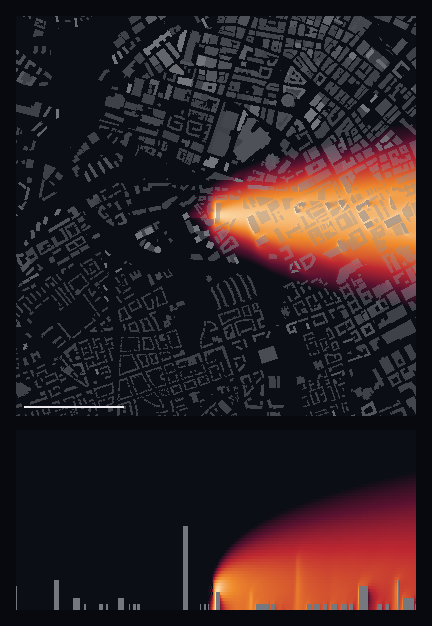
\includegraphics[width=0.82\textwidth]{fig/urban_mcr_plume.png}
\caption{Urban plume over Manchester city centre after five minutes of
continuous release from a rooftop at $32.5$~m. \emph{Top}: plan view, building
footprints in grey, column-integrated concentration on a logarithmic scale; the
bar is $500$~m. \emph{Bottom}: vertical section along the plume centreline,
vertical scale exaggerated three times, showing the release lifting as it enters
faster-moving air aloft. The wind is a $5\,\mathrm{m\,s^{-1}}$ westerly, so the
plume runs east. Note what the figure does \emph{not} show: the wind is
prescribed, so there is no recirculation behind any of these buildings and no
channelling along the streets the plan view makes so visible.}
\label{fig:urbanplume}
\end{figure}

\paragraph{A second configuration, and what the first one hid.} Releasing at the
centre of the domain into a due-east wind gives only $1$~km of fetch, and the
plume reaches steady state at $t=5$~min --- three fifths of that run is static.
Moving the source to an open pocket in the south-west at $(140,135)$~m and
turning the wind onto the diagonal, toward the north-east, gives $2.6$~km of
fetch; steady state then arrives at $10.8$~min and the plume develops throughout.
The source also sits at street level, $7.5$~m, rather than being lifted onto a
roof as the central cell was.

That change exposed a defect the first configuration could not. The count of
cells used to normalise the release and the set of cells actually injected into
were separate predicates, and they disagreed at $z=0$: the count required
$z>0$ while the injection covers every bulk cell, which since
\S\ref{sec:urban} includes the ground layer. A box centred at $z=1$ therefore
had its per-cell rate computed for three layers and applied to four --- $33\%$
over-injection, visible within eighteen seconds as more scalar in the domain
than had been released, and invisible for any source clearing $z=2$. The two are
now one named predicate, asked twice.

The diagonal wind appears to cost stability margin: zeroing both horizontal
components inside buildings raises $\max|\nabla\!\cdot\!\uu|$ from
$2.3\times10^{-2}$ to $3.3\times10^{-2}$, and the max-based margin of
\S\ref{sec:urbanstab} falls from $7.2$ to $5.1$. That was described here as
``comfortably clear of the $1.8$ that diverged'', on the strength of a mass
budget that stayed sensible for the whole run --- which, as \S\ref{sec:urbanstab}
now records, is not a judgement a mass budget can make.

The configuration was therefore repeated and its undershoot examined. It is
stable, and not marginally so: $\min C$ is bit-identical at $-1.11\times10^{-7}$
for six consecutive frames from $t=45$ to $t=120$~s, while a Manhattan run at
nominally the same margin had grown its undershoot twentyfold over the same span.
What the max-based number was hiding is that the diagonal wind barely changes the
rms at all --- $9.42\times10^{-4}$ to $9.21\times10^{-4}$, a $2\%$ \emph{fall} ---
because it redistributes divergence among the same wall-adjacent cells rather
than adding any. On the statistic that predicts the outcome this is the safest
configuration in the table, at $180\times$.

\paragraph{Negative concentrations.} The scheme undershoots. A first-order
equilibrium with no limiter produces small negative concentrations at sharp
gradients: $3.2$~million cells of $9.6$~million hold values between $0$ and
$-7.9\times10^{-5}$, against a section peak of $5.4\times10^{-2}$ --- a few
parts in ten thousand. They are bounded and do not grow, and \texttt{min C} is
now reported every frame so that they are visible rather than assumed away. The
practical consequence is for anything downstream that takes a logarithm or
treats a negative value as a flag: the plan-view renderer for
Figure~\ref{fig:urbanplume} initially tested \texttt{v < 0} for the building
mask, which is how it came to paint three million undershooting cells as
buildings and hide most of the city.

\subsection{A second city}
\label{sec:urbannyc}

Midtown Manhattan, $400\times400\times100$ cells at $5$~m --- the same $2$~km
square, $500$~m deep, $10\,210$ buildings --- with the same
$5\,\mathrm{m\,s^{-1}}$ wind at $10$~m and $z_0=1$~m, and the same continuous
release of one unit per second from street level at $7.5$~m. Everything that
could be held fixed against \S\ref{sec:urban} was. What could not is the
diffusivity: $D=35\,\mathrm{m^2s^{-1}}$ against Manchester's $20$, for the
reason \S\ref{sec:urbanstab} sets out. Fifteen minutes of physical time is
$46\,665$ steps and $51$ frames.

\begin{figure}[htbp]
\centering
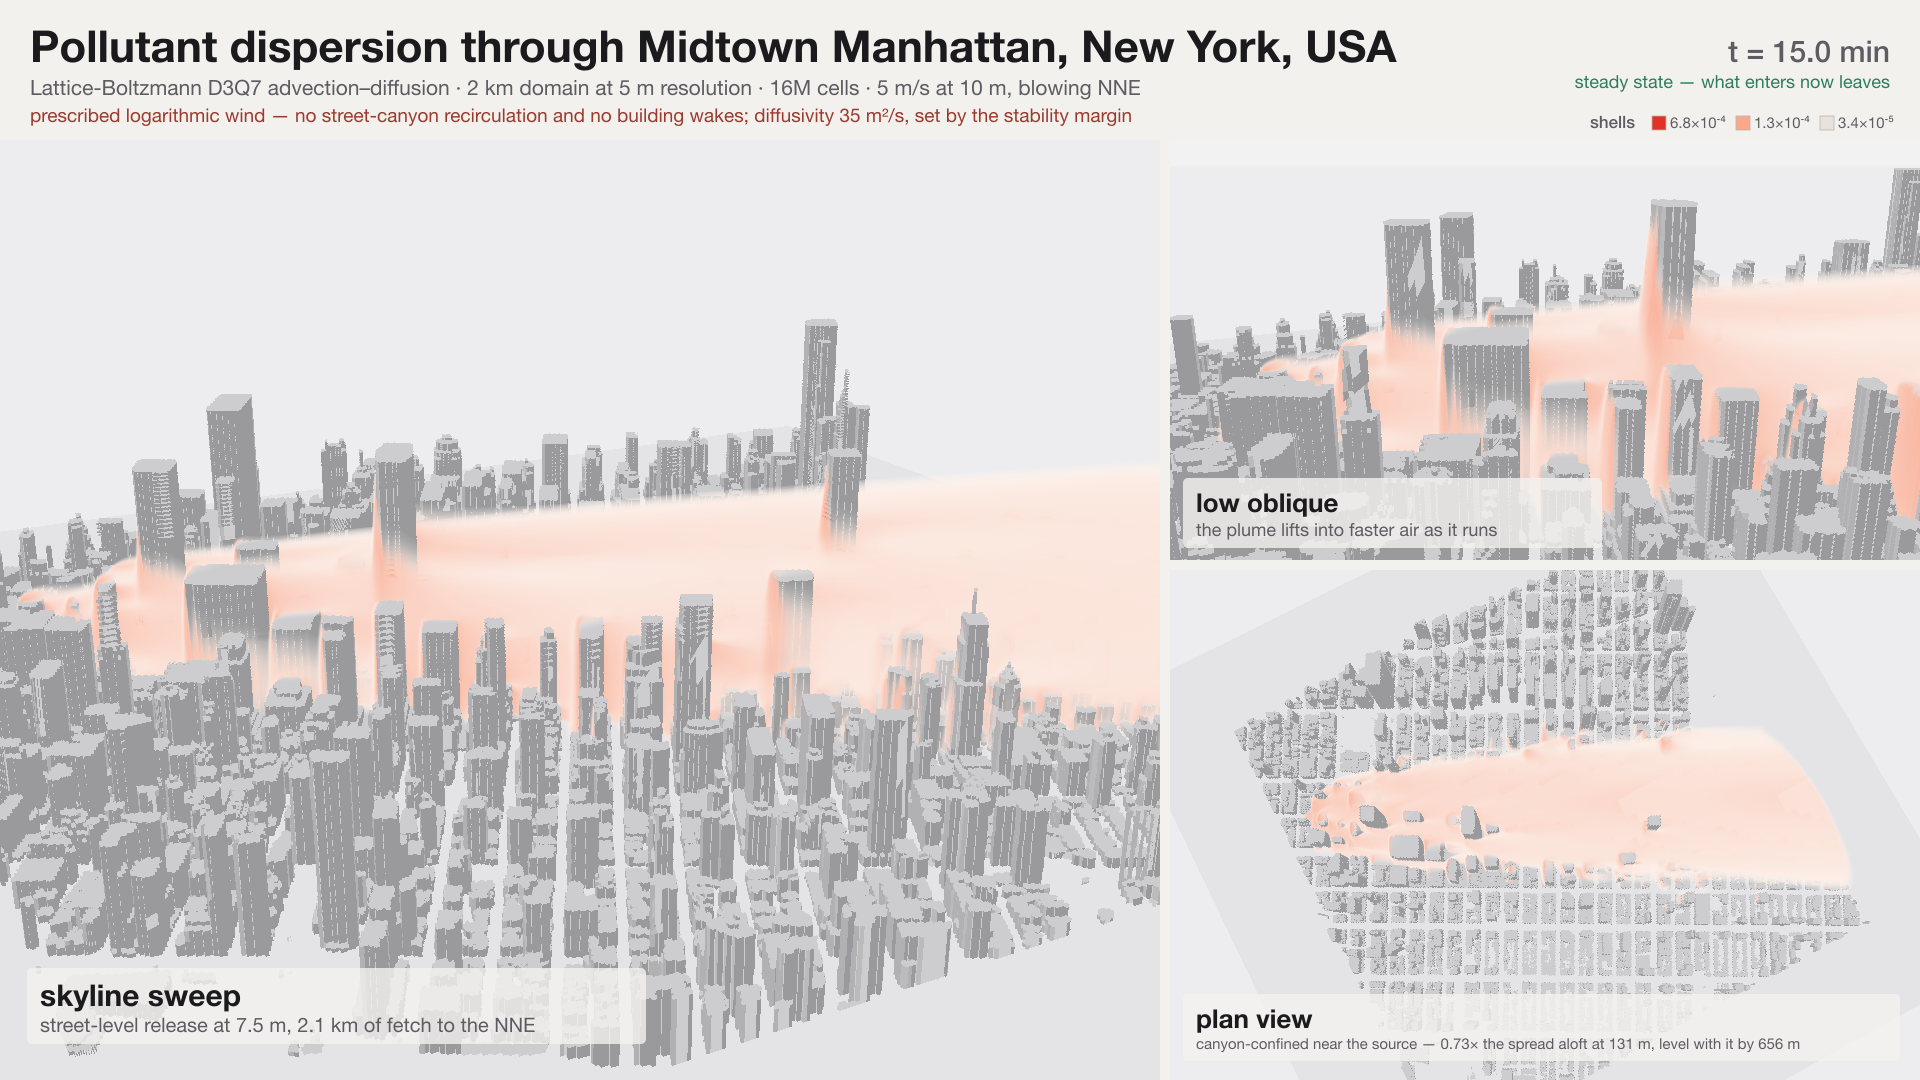
\includegraphics[width=\textwidth]{fig/urban_nyc_collage.png}
\caption{Midtown Manhattan at steady state, fifteen minutes into a continuous
street-level release. Three shells of concentration, at the levels enclosing
$95\%$, $80\%$ and $50\%$ of the plume's mass --- chosen from this frame rather
than carried over from another run, since the same release spread over $2$~km
carries an order of magnitude less than it does over $200$~m. \emph{Left}: the
skyline broadside to the plume, which runs left to right along the avenues.
\emph{Top right}: the same view from street level, showing the release
threading between the towers. \emph{Bottom right}: plan view, with the
Commissioners' grid visible; the wind bearing was measured out of the height
field, not looked up. Every figure in the caption strip is read from the run's
own log, and the plan-view line is measured from this frame. The animation is
\texttt{doc/fig/manhattan\_dispersion.mp4}.}
\label{fig:urbannyc}
\end{figure}

\paragraph{The wind direction was measured, not assumed.} Manhattan's street
grid is not aligned with north, and rather than look the angle up it was
recovered from the height field: rays marched from every open column, in every
direction, recording how far they travel before meeting a building. The mean
free run peaks at two orthogonal bearings, $28^\circ$ and $118^\circ$ --- $385$~m
along the second, $285$~m along the first --- which is the Commissioners' Plan of
1811, extracted from a $400\times400$ array of heights with no knowledge of what
city it is. The wind was then aimed along $28^\circ$, up the avenues, giving
$2.10$~km of fetch from a source in an open pocket in the south of the domain.

\paragraph{Steady state, and a budget that now says what it means.} The plume
reaches steady state at about $11.4$~min, where $\mathrm{d}M/\mathrm{d}t$ falls
below $2\%$ of the injection rate; by the last frame it is $1.8\times10^{-3}$ and
the mass in the domain has plateaued at $3.670\times10^{2}$ against
$8.817\times10^{2}$ injected. That $41.6\%$ retained is a real statement about
where the release has gone --- the remaining $58\%$ has left through the outlets
--- which it was not before \S\ref{sec:wallslots}: the same run reported under the
old fluid-only sum would have shown $87\%$ and held there while the plume was
still in the middle of the domain. The companion column reads $92.0\%$ for the
whole run, unchanging: that is the fraction the plotted field sees, and the $8\%$
gap is Manhattan's wall area.

The undershoot is $-8.08\times10^{-9}$ and does not move for any of the $51$
frames --- the total negative mass is $3\times10^{-7}$, or $0.00\%$ of the plume.
At $D=20$ the same configuration reached $-1.3\times10^{-2}$ by $t=162$~s and was
doubling every eighteen seconds.

\paragraph{The canyons hold the plume, but only near the source.} The plan view
of a city plume invites a claim about street channelling, and the caption on the
Manchester animation made one: \emph{isotropic lateral spread --- the streets do
not steer it}. On a regular grid of canyons with the wind aimed along one of its
axes that is worth measuring rather than asserting, so
\texttt{doc/fig/plume\_stats.py} bins the last frame by downwind distance along
the plume's own axis and compares the concentration-weighted crosswind spread
below and above the rooflines:

\begin{center}
\begin{tabular}{rccccc}
\toprule
$s$ (m) & $\sigma_n$ street & $\sigma_n$ aloft & ratio &
$\langle z\rangle$ street & street fraction \\
\midrule
 131 & $39.5$  & $53.8$  & $0.73$ & $26.2$ & $75.5\%$ \\
 394 & $57.7$  & $72.1$  & $0.80$ & $31.5$ & $47.8\%$ \\
 656 & $78.1$  & $80.6$  & $0.97$ & $31.9$ & $33.8\%$ \\
 919 & $99.3$  & $94.9$  & $1.05$ & $32.1$ & $32.4\%$ \\
1181 & $99.8$  & $99.9$  & $1.00$ & $33.2$ & $25.7\%$ \\
1706 & $120.0$ & $123.0$ & $0.98$ & $31.3$ & $22.7\%$ \\
1969 & $130.3$ & $120.4$ & $1.08$ & $33.0$ & $19.7\%$ \\
\bottomrule
\end{tabular}
\end{center}

\noindent Within the first $130$~m the plume is $27\%$ narrower below the
rooflines than above them, and by $650$~m the two are the same. The last column
says why: the fraction of the plume still below roof level falls from $76\%$ to
$20\%$, so there is progressively less left for the canyons to hold. The
street-level material that remains does not rise --- its mean height sits at
$32$~m the whole way --- while the part aloft climbs from $91$~m to $164$~m as it
mixes into faster air.

That is a confinement effect and \emph{not} a channelling one, and the
distinction matters here more than it would in a solved wind. The prescribed
field blows in a straight line by construction: nothing in this model can steer
a plume along a street. What the buildings do is block, and being opaque to the
scalar is on its own enough to produce the near-field narrowing. A solved wind
would add the channelling this one cannot represent, and the honest reading of
the table is as a lower bound on how much the geometry matters.

The caption on the animation is generated from exactly this measurement rather
than written by hand, for the reason the Manchester caption illustrates: pointed
at a second city, a caption made of literals states the first city's name, cell
count and fetch with complete confidence.

\subsection{Solving the wind}
\label{sec:urbansolved}

The wind can instead be solved: D3Q27 TRT Navier--Stokes on the same geometry,
sharing the Domain, $\Delta x$ and $\Delta t$ with the scalar, so the fluid's
lattice velocity \emph{is} the scalar's and the two couple with no conversion.
TRT rather than BGK because the effective viscosity puts $\tau^+$ within a few
thousandths of $1/2$, where BGK is unusable and TRT's free antisymmetric rate is
exactly the lever required; $\Lambda = 3/16$ additionally places the
bounce-back wall halfway, so a voxelised building is the size it looks. Starting
from the undisturbed profile rather than from rest leaves only the wakes to
develop, and the solve converges to a relative change of $2\times10^{-7}$ in
$7000$ steps.

\begin{figure}[htbp]
\centering
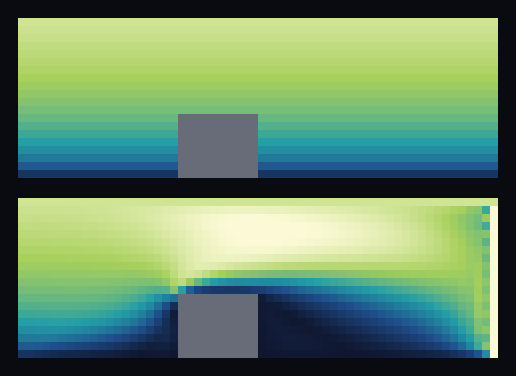
\includegraphics[width=0.78\textwidth]{fig/urban_wind_compare.png}
\caption{Vertical section through a building, wind speed, both panels on the
same scale. \emph{Top}: the prescribed logarithmic profile --- flat horizontal
layers, unaware that the building is there. \emph{Bottom}: the solved field ---
upstream stagnation, acceleration over the roof, and a slow wake in the lee
recovering over roughly twenty cells. Along the centreline at mid-building
height the prescribed field is $4.34\,\mathrm{m\,s^{-1}}$ everywhere, while
the solved one falls to $1.37$ approaching the building and $0.30$ behind it.
The bright stripe at the right edge is the outlet-corner artefact discussed
below, left visible rather than cropped. The colour scale is the $98$th
percentile, not the maximum: that artefact reaches $29\,\mathrm{m\,s^{-1}}$ and
scaling to it renders every physical feature in the bottom quarter of the ramp
--- the same trap as the aorta volume render, where $p_{100}$ was $2.7$ times
$p_{99.9}$.}
\label{fig:urbanwind}
\end{figure}

\paragraph{The interior is right, and is the point.} \emph{All the figures in
this and the next paragraph are the synthetic $60\times30\times20$ case}, which
for a long time was the only geometry this mode had ever been run on; the city
results are in \S\ref{sec:urbansolvedcity}. Three cells clear of every
face, the divergence falls from $\mathrm{RMS} = 1.27\times10^{-3}$ prescribed to
$2.12\times10^{-4}$ solved --- a factor of six --- and the peak speed is
$8.80\,\mathrm{m\,s^{-1}}$ against a $7.74\,\mathrm{m\,s^{-1}}$ free stream, a
$14\%$ speed-up over the building. That is a result the prescribed profile
cannot produce at all, and the divergence drop is the spurious source of
\S\ref{sec:urbanstab} shrinking, which is what drove both the concentration
error and the stability floor.

\paragraph{The domain edges are not right.} Where the pressure outlet meets the
velocity-prescribed lateral and top faces the corner is over-determined, and a
jet forms along it: $31.6\,\mathrm{m\,s^{-1}}$ and
$\nabla\!\cdot\!\uu = 9.5\times10^{-2}$, against $8.8$ and $7.0\times10^{-3}$
in the interior. This is why the global maxima look worse than the prescribed
field's while every interior statistic is better, and it is the reason the
diagnostics now report interior-only figures and say whether the worst
divergence sits on a domain face --- without which the two were not separable.

Two remedies were tried. Giving the edges the free-stream profile removed the
sixty-eight inert outflow nodes, whose donor lay on an adjoining wall, but did
\emph{not} remove the jet, which locates the cause in the mixed condition
itself rather than in the donor lookup. The identified fix is periodic lateral
boundaries, the standard atmospheric arrangement, which deletes two of the four
offending faces outright.

\subsection{The same mode on a city, and the two things that stopped it}
\label{sec:urbansolvedcity}

Everything above is the synthetic case. Pointed at Manchester the mode produced
a NaN within $500$ steps --- in FP64 as well as FP32, so not a precision effect
--- and it did so at the $\tau^+$ the synthetic case had converged at. Bisecting
by geometry:

\begin{center}\small
\begin{tabular}{lccll}
\toprule
case & buildings & on faces & outcome & peak / free stream \\
\midrule
synthetic $60\times30\times20$   & 1    & no  & converges, $5.7\times10^{-7}$    & $4.1\times$ \\
flat $200\times200\times150$     & none & --- & no NaN, residual $6.5\times10^{-2}$ & $4.4\times$ \\
Manchester $400\times400\times60$ & 6058 & \textbf{yes} & \textbf{NaN by step 500} & --- \\
Manchester, 8-cell clear margin  & 2083 & no  & no NaN, residual $2.7\times10^{-1}$ & $2.6\times$ \\
\bottomrule
\end{tabular}
\end{center}

\paragraph{A face cell shadowed by a building is ill-posed.} The regularised
condition reconstructs the density at a wall node from the populations that
streamed into it, split by the wall normal into known and unknown, and that
split assumes the known ones arrived from the interior. When the cell one step
inward is a building, what actually arrives is bounce-back off that building,
the reconstructed density is not a density, and the solve diverges. Manchester
has $3975$ built columns touching the domain edge; clearing an eight-cell band
removes the NaN outright, which is what identified the cause. Only $141$ cells
are \emph{actually} shadowed --- a face cell with solid immediately inward ---
and those $141$ were enough to destroy a nine-million-cell solve. They are now
closed as \texttt{Solid}, which extends the building by the one cell it was
already effectively occupying and turns an ill-posed node into a well-posed
wall. That also subsumes the ``outflow node has no fluid neighbour and is
inert'' case: the same geometry seen from the outlet side, previously left
frozen rather than closed.

\paragraph{Periodic laterals, and what they cost.} \texttt{-lateral periodic}
makes the $y$ faces periodic, deleting two of the four junctions where a
velocity-prescribed wall meets a pressure outlet. Periodicity is handled inside
\texttt{Domain::fill\_neighbours}, so neither solver needed changing; the
divergence diagnostics did, because $y=0$ and $y=n_y-1$ become ordinary
interior cells whose neighbours wrap, and omitting them would drop $0.5\%$ of
the domain from an rms the stability threshold is built on.

The two fixes are independent, and it is worth being explicit that periodic
laterals alone do \textbf{not} cure the NaN --- they leave the inlet and outlet
faces, where the same shadowing occurs. Both are required.

What periodicity costs is a modelling choice rather than accuracy, and the run
now states it rather than leaving it implicit: the domain becomes an infinite
strip, the city repeats every $2$~km across the wind, and a plume drifting
sideways out of one edge re-enters at the other. The seam is not smooth either,
since real building heights at $y=0$ and $y=n_y-1$ were never chosen to match:
$220$ of Manchester's $400$ edge columns disagree, worst by $48$~m. That count
is printed, and a separate warning fires if the wind has a cross-wind component,
because the plume is then advected through the seam rather than merely diffusing
across it.

\paragraph{A solved wind inverts which statistic misleads.} With both fixes,
Manchester at $8000$ flow steps --- one flow-through time at
$u^{\max}_{\rm lat} = 0.05$, so a developing field and not a converged one:

\begin{center}\small
\begin{tabular}{lccc}
\toprule
 & prescribed & solved & change \\
\midrule
rms, whole domain      & $9.422\times10^{-4}$ & $2.638\times10^{-3}$ & $0.4\times$ \\
rms, 3 clear of a face & $9.614\times10^{-4}$ & $7.401\times10^{-5}$ & $\bm{13.0\times}$ \\
rms, wall-adjacent     & $8.407\times10^{-3}$ & $2.045\times10^{-3}$ & $4.1\times$ \\
max, whole domain      & $2.318\times10^{-2}$ & $8.351\times10^{-2}$ & $0.3\times$ \\
max, 3 clear of a face & $2.318\times10^{-2}$ & $1.016\times10^{-2}$ & $2.3\times$ \\
\bottomrule
\end{tabular}
\end{center}

\noindent The interior is $13\times$ better, more than double the factor of six
the synthetic case showed. The global figures are $2.8\times$ \emph{worse}, and
the worst cell sits at $(398,342,58)$: the outlet/top edge, the one junction
periodic laterals cannot delete.

So the two fields fail differently, and the statistic that reads correctly for
one misreads the other. A prescribed field spreads its error through the city,
so its whole-domain and interior rms agree to $2\%$ ($9.42\times10^{-4}$ against
$9.61\times10^{-4}$, margins $44\times$ and $43\times$) and the test of
\S\ref{sec:urbanstab} is the whole story. A solved field is divergence-free
everywhere it is solved and carries its entire error at one boundary, so the
whole-domain figure is set by that edge and understates the interior by more
than an order of magnitude: $16\times$ against $561\times$. Both are now
printed, the run says so explicitly when they differ by more than a factor of
three, and the warning stays on the whole-domain figure because only that one is
a guarantee.

\paragraph{The diffusivity floor is a property of the prescribed profile.} This
is what solving the wind buys, stated at the diffusivity that matters.
$D = 5\,\mathrm{m^2s^{-1}}$ is the value that diverged under the prescribed
wind, at an interior margin of $43\times$. Under the solved wind the same
$D = 5$ gives $561\times$. Every urban run in this document has been constrained
to $D \geq 20$ by a term that the wind model introduced and the physics does
not contain.

Two caveats stand. The field above is one flow-through time, not a converged
urban wind --- three to five would be the usual requirement, and at the measured
rate on this machine that is four to seven hours. And the outlet/top edge is
still over-determined, so a plume must be kept clear of it. The prescribed wind
therefore remains the default.

\subsection{Coupling the wind, unsteadily}
\label{sec:urbanunsteady}

Everything in \S\ref{sec:urbansolvedcity} freezes the wind: solve once, hand the
converged field to the scalar, transport. A converged field has a steady
recirculation behind every building, and a steady recirculation stirs nothing
--- so nothing in a frozen-wind run can show the plume being torn apart by a
building's wake, only advected around its time-averaged shape. \texttt{-mode
unsteady} spins the flow up as before and then advances it \emph{one step per
scalar step}, refreshing \texttt{ux/uy/uz} in place: they are the very Views the
scalar was handed, so the refresh \emph{is} the coupling and nothing is copied.
The added cost is one \texttt{compute\_macroscopic} pass per step, which is the
price of an instantaneous rather than a mean field.

\paragraph{A crop, and a viscosity found the hard way.} A coupled run costs a
flow step every scalar step, so the full $2$~km city is hours rather than
minutes; a $1\times0.75$~km, $200\times150\times60$ crop at the same $5$~m
resolution keeps what resolves the wakes and spends the saving on footprint.
The crop was chosen for density, not the emptiest corner: a $169$~m tower, the
tallest in the whole city, sits inside it, together with $49\%$ of columns
built. The obvious first choice happened to put that tower on the periodic
seam, wrapping it into itself; moved $30$~m, the seam mismatch on the tallest
column falls from $169$~m to $42$~m.

Effective viscosity had to be found rather than assumed. $\nu=2$ and $\nu=4\,
\mathrm{m^2s^{-1}}$ both NaN on the crop; $\nu=8$ runs. During spin-up its
residual oscillates --- $8.2\times10^{-3}$ at $4000$ steps against
$7.0\times10^{-2}$ three hundred steps earlier --- and it was tempting to read
that as an unsteady field. It is not. \textbf{The flow settles.} Measured
between consecutive output frames, four seconds apart, once the coupling is
running:

\begin{center}\small
\begin{tabular}{lccc}
\toprule
frames & $\mathrm{rms}|\uu_{i+1}-\uu_i|$ & as \% of $\mathrm{rms}|\uu|$ & max \\
\midrule
$30\!\to\!31$ & $1.66\times10^{-3}$ & $0.015\%$ & $0.022$ \\
$31\!\to\!32$ & $1.37\times10^{-3}$ & $0.012\%$ & $0.014$ \\
$45\!\to\!46$ & $5.5\times10^{-4}$  & $0.005\%$ & $0.006$ \\
$59\!\to\!60$ & $3.2\times10^{-4}$  & $0.003\%$ & $0.005$ \\
\bottomrule
\end{tabular}
\end{center}

\noindent Monotonically decaying to three parts in a hundred thousand. The
oscillating spin-up residual was a decaying transient, not shedding, and the
field the plume rides is steady to within round-off by the end. At $\nu=8$ the
$169$~m tower sits at $Re\approx250$ on its own width, which is enough for a
free-standing bluff body to shed --- but this one is wall-mounted in a rough
boundary layer among neighbours, and at $6.7\times10^{-3}$ lattice viscosity the
shear layers are damped before they can roll up. Reaching a shedding regime
needs a lower viscosity, and $\nu=4$ is where this configuration stops
converging at all. \textbf{That is the gap: between the viscosity at which the
solve survives and the viscosity at which the flow becomes unsteady, there is
currently no overlap on this geometry.}

So this section demonstrates that the coupling MECHANISM works --- the flow
advances with the scalar, the plume rides an instantaneous field, and $D=5$ is
stable throughout --- and does not demonstrate turbulent dispersion. What the
plume experiences here is a steady solved wind with recirculation and
channelling, which is still something no prescribed profile can produce, and is
not turbulence.

\begin{figure}[htbp]
\centering
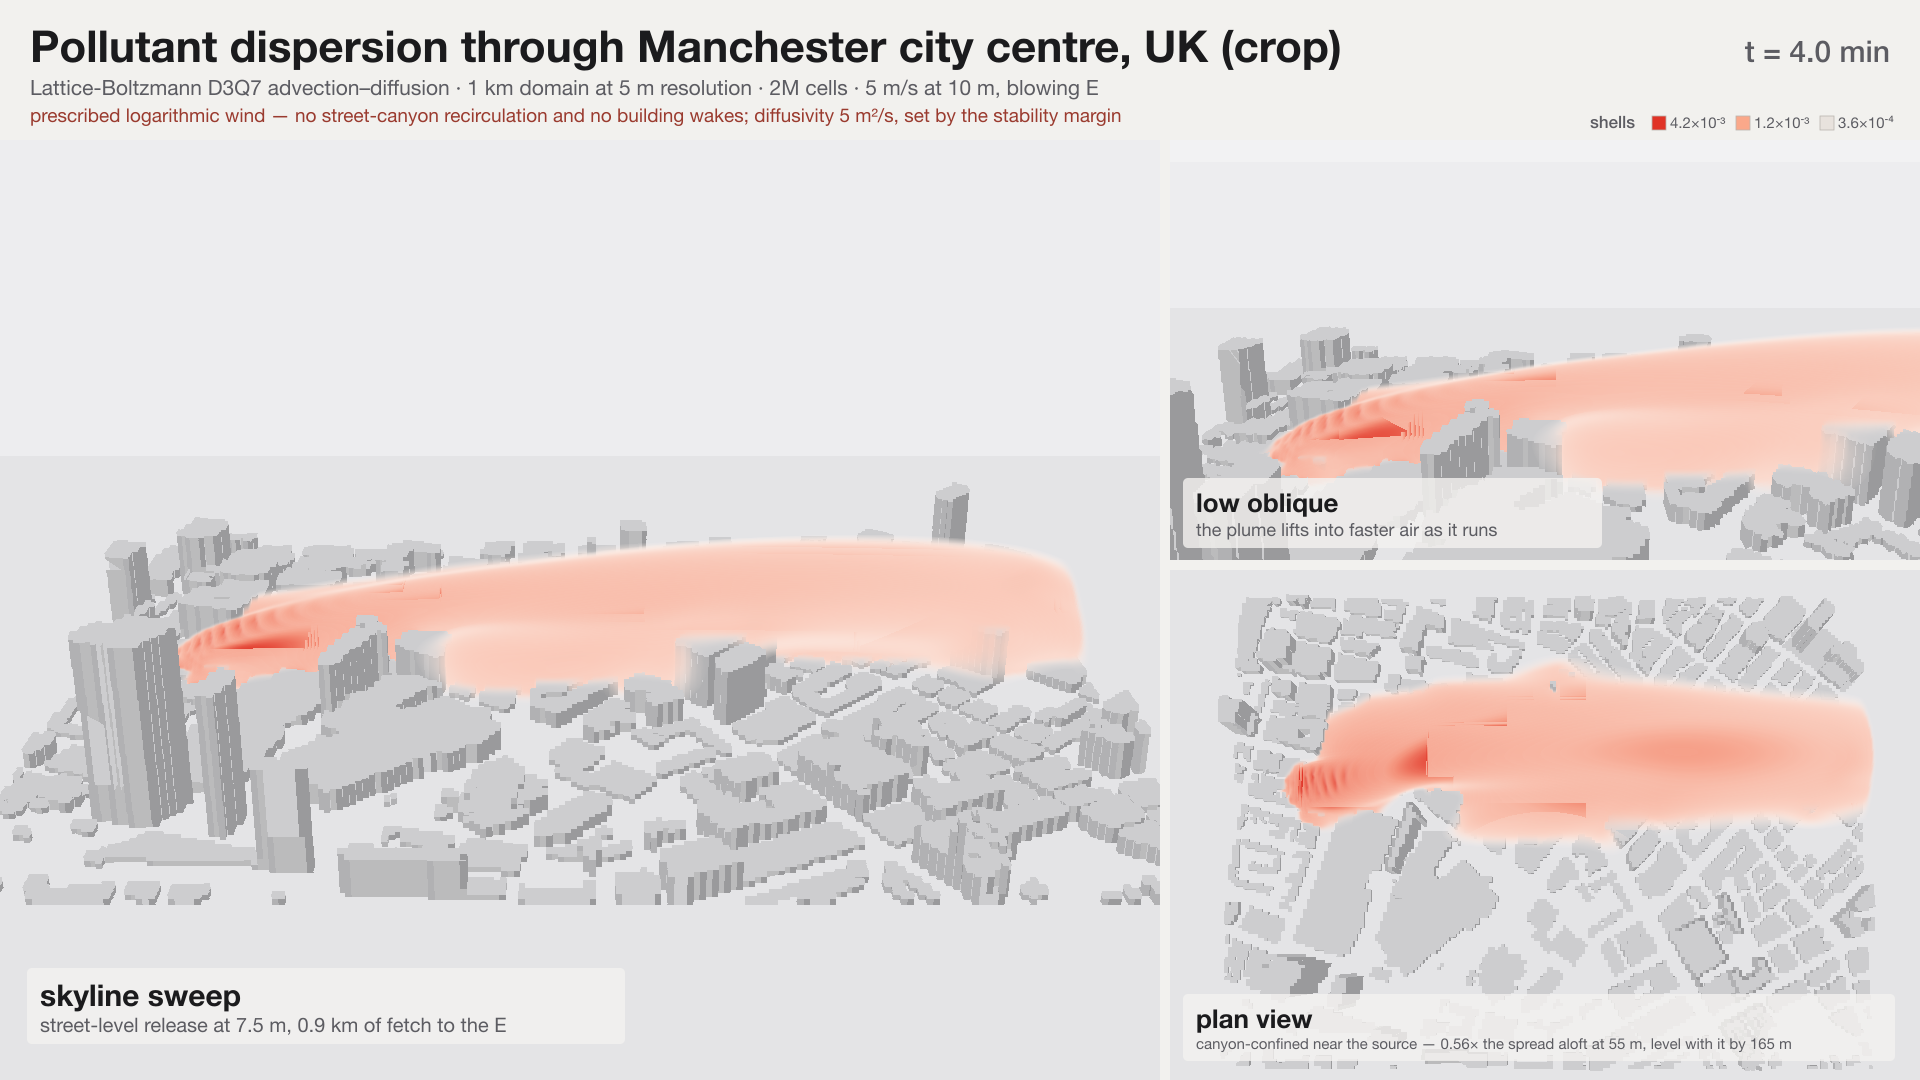
\includegraphics[width=\textwidth]{fig/urban_mcr_coupled_collage.png}
\caption{Coupled dispersion, Manchester crop, $3.7$~min into a street-level
release at $7.5$~m with $0.9$~km of fetch, at
$D=5\,\mathrm{m^2s^{-1}}$ --- the value that diverged outright under the
prescribed wind (\S\ref{sec:urbanstab}). The flow is advanced one step per
scalar step, but it converges rather than shedding (above), so the plume is
riding a steady solved wind, not a turbulent one. The animation is
\texttt{doc/fig/mcr\_coupled\_unsteady.mp4}.}
\label{fig:urbancoupled}
\end{figure}

\paragraph{$D=5$ is comfortable, not marginal.} Under the prescribed wind this
diffusivity diverged outright. Coupled and unsteady, $\min C$ --- the early
warning of \S\ref{sec:urbanstab} --- holds at $-2.5\times10^{-4}$ for the entire
second half of a four-minute release, drifting by less than $3\%$ step to step
despite riding on a field that is itself fluctuating by tens of per cent. The
interior divergence is $319\times$ the damping rate against the prescribed
field's $43\times$ at the same $D$, and the peak interior speed is $15.4\,
\mathrm{m\,s^{-1}}$ against an $11.9\,\mathrm{m\,s^{-1}}$ free stream --- a
$29\%$ speed-up over the buildings, against $14\%$ in the converged synthetic
case of \S\ref{sec:urbansolved}. An unsteady field is not merely divergence-free
on average; the instant-by-instant acceleration over a roof is larger than a
time-averaged solve ever shows.

\paragraph{The confinement result reverses.} \S\ref{sec:urbannyc} found Manhattan's
plume narrower below the rooflines than above near the source, widening to equal
by $650$~m --- confinement, from buildings simply blocking a wind that cannot
itself be steered. Measured the same way here:

\begin{center}\small
\begin{tabular}{rccc}
\toprule
$s$ (m) & $\sigma_n$ street & $\sigma_n$ aloft & ratio \\
\midrule
 55  & $23.6$ & $42.2$ & $0.56$ \\
165  & $30.0$ & $24.9$ & $1.20$ \\
275  & $41.9$ & $32.5$ & $1.29$ \\
385  & $52.3$ & $37.5$ & $\bm{1.39}$ \\
495  & $51.7$ & $42.8$ & $1.21$ \\
605  & $42.1$ & $43.4$ & $0.97$ \\
\bottomrule
\end{tabular}
\end{center}

\noindent The ratio rises \emph{above} one in the near-to-mid field before
settling back near it: the street-level plume spreads sideways \emph{faster}
than the air above the roofs, rather than merely failing to be confined.

The cause is steady recirculation, not turbulence --- the field is steady, as
measured above. A prescribed profile is zeroed inside buildings and otherwise
flows straight, so it can only fail to confine; a solved field has standing
lateral recirculation in the lee of every block, and that alone moves material
across the flow faster than diffusion does. It is a weaker claim than turbulent
dispersion and it is the one the data supports. Row one, at $s=55$~m, is still
the source's immediate vicinity and reads like the confined case of
\S\ref{sec:urbannyc} for the same reason --- the plume has not yet reached a
recirculation zone.

This is one release over four minutes on one crop, and the numbers above should
be read as a demonstration that the mechanism is there and measurable, not as a
converged statistic. \texttt{-mode unsteady} is new in this section and has had
one city and one geometry through it --- and, as recorded above, has not yet
been run at a viscosity where the flow is actually unsteady.

\begin{figure}[htbp]
\centering
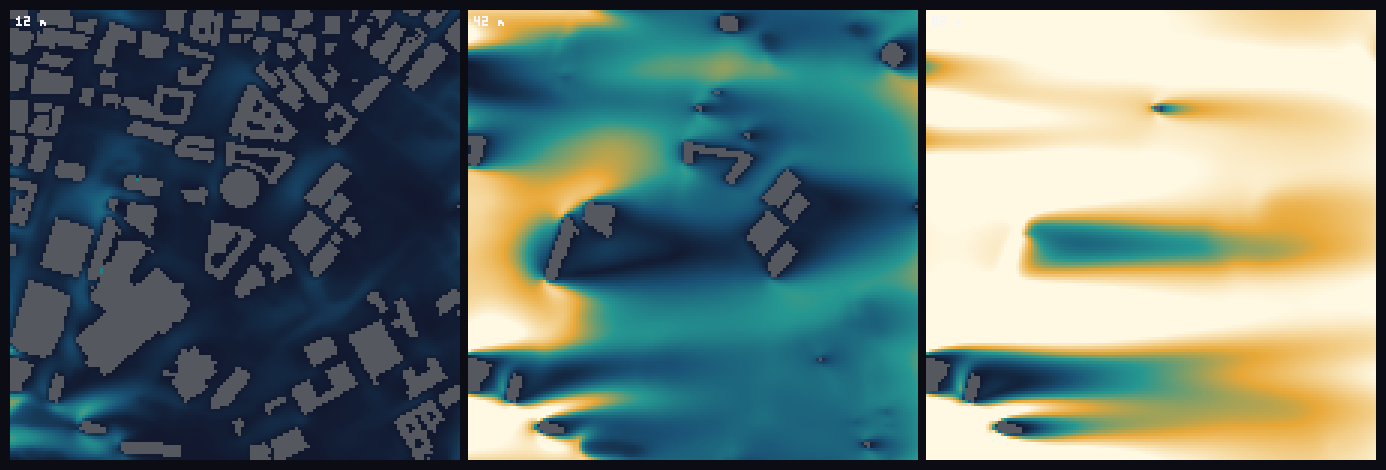
\includegraphics[width=\textwidth]{fig/urban_wind_3heights.png}
\caption{The solved wind at three heights: $12$~m inside the canyons,
$42$~m around roof level, $82$~m in the free stream. One colour scale across
all three, so they are comparable --- dark is slow. The wake streaks trailing
downwind of the tall blocks in the $82$~m panel are the structure a volume
render could not show: a wake field is a boundary layer that fills the lower
domain, $45\%$ of fluid cells carrying a positive velocity deficit, so
front-to-back compositing accumulates along every ray and returns an opaque
slab at any threshold. Stacked slices work where shells do not. The animation
is \texttt{doc/fig/mcr\_wind\_3heights.mp4}.}
\label{fig:urbanwind3h}
\end{figure}

\subsection{The top boundary is a modelling choice}

A horizontal wind has $u_z = 0$ at the top face, so a zero-gradient condition
there passes no advective flux --- there is none --- and no diffusive flux,
because that is what zero-gradient means. The top is therefore a \emph{lid}:
material that mixes to it stays in the domain. That is right when the top is far
above the plume and wrong when it is not. Holding the top at $C=0$ instead says
the atmosphere above is clean and lets the scalar diffuse into it, which is the
more physical statement for a domain whose top is an arbitrary cut through the
boundary layer, at the cost of forcing $C=0$ there. Both are offered; the lid is
the default because it is the validated condition. On the synthetic case the
choice is worth $0.7\%$ of retained mass, which is small only because the plume
does not reach the top --- it is not a general bound.


%==============================================================================
\section{A second implementation, in CUDA}
\label{sec:cuda}

Everything measured so far in this document is the Threads backend. This section
records what happened when the code was taken to a GPU, why that made a second
implementation necessary, and what the second implementation then measured.

\subsection{The result that forced the question}
\label{sec:cmcollapse}

On a Tesla T4 (sm\_75, CUDA 12.8, FP32), seven validation executables build and
run after six separate fixes for \code{nvcc} restrictions that neither the Serial
nor the Threads backend can see. All six are committed with explanatory comments,
and they are worth listing because any future port will meet them:

\begin{enumerate}[leftmargin=1.4em,itemsep=2pt]
\item A kernel-launching member function may not be private: an extended
  \code{\_\_host\_\_ \_\_device\_\_} lambda's enclosing function must not have
  private or protected access.
\item A variable may not be first-captured inside an \code{if constexpr}. In
  \code{run\_step} this was repaired with a plain \code{if}, which still folds
  because the tested value is a compile-time constant.
\item The same restriction in the wall closure, where a plain \code{if} does
  \emph{not} work: the captured member does not exist in the unforced
  instantiation, so the object has to be named before the branch.
\item Lattice constants declared \code{static constexpr int cx[Q]} are
  unreachable from device code when indexed at runtime. They are now
  \code{KOKKOS\_INLINE\_FUNCTION} accessors wrapping function-local arrays.
  \textbf{Invariant to preserve: \code{src/} contains no static constexpr array
  members.}
\item The same, in \code{MonomialBasis}.
\item Extended lambdas may not appear inside a \emph{generic} lambda, and
  function-local types may not be template arguments of one.
\end{enumerate}

\noindent BGK and TRT then reach $420$--$447$ MLUPS at $64^3$, with mass drift
\textbf{exactly $0.000\e{0}$} on every row --- about $8.4\times$ the M1 Threads
figure of \S\ref{sec:perf}.

\paragraph{But the central-moment operators do not run.} The two
\code{MomentCollision} configurations did not finish in \textbf{seventeen
minutes} at $64^3$ over 50 steps, against $\sim0.03$\,s for BGK. That is roughly
four orders of magnitude and it is not explained. The obvious hypothesis was
register spilling, and \code{-Xptxas -v} rules it out: \textbf{zero spill bytes},
largest stack frame 96 bytes, 116 registers per thread. Occupancy at 116
registers is about $25\%$ on a T4 --- a real effect, and far too small a one.

This matters more than a performance note. The aorta demonstrator and the whole
validation campaign of \S\ref{sec:campaign} run central moments, so the $447$
MLUPS is a \textbf{BGK-only} figure and must not be quoted as this code's GPU
throughput.

\paragraph{Which leaves one question.} Is the collapse a property of the
\emph{algorithm} --- 27 moments, two transforms and a relaxation schedule per
node --- or of \emph{this code's route to the device}? Nothing in the Kokkos
implementation can answer that, because every hypothesis is tested against the
same code. The only decisive experiment is a second implementation.

\subsection{The answer}

\code{GPU/} is that experiment: a lattice Boltzmann solver written directly in
CUDA, sharing no headers with \code{src/}, not built by the parent
\code{CMakeLists}, and not a port. Only the physics and the output format are
deliberately the same, which is what makes the comparison mean anything.

\begin{center}\small
\begin{tabular}{llrrr}
\toprule
device & operator & grid & MLUPS & GB/s \\
\midrule
Tesla T4  & BGK             & $128^3$ & 950.2  & 205.2 \\
Tesla T4  & central moments & $128^3$ & 950.4  & 205.3 \\
NVIDIA H200 & BGK             & $512^3$ & 17233.4 & 3722.4 \\
NVIDIA H200 & central moments & $512^3$ & 17171.4 & 3709.0 \\
\bottomrule
\end{tabular}
\end{center}

\noindent The H200 rows were measured by Yang; see \S\ref{sec:h200}. Mass drift
is exactly $0.000\e{0}$ on every row. Central moments runs
at $99.6\%$ of BGK on two card generations, and $3722$\,GB/s is $77.3\%$ of the
H200's $4814$\,GB/s peak --- i.e.\ the kernel is memory-bound, which is what a
correctly written lattice Boltzmann kernel should be. Taylor--Green at $512^3$
(134M nodes, 256\,000 steps) completes in 2046\,s.

\textbf{So the collapse of \S\ref{sec:cmcollapse} is not the algorithm.} The same
27-moment separable transform, the same relaxation schedule and the same Esoteric
Pull run at BGK speed when written directly. Whatever is wrong is in how the
Kokkos code reaches the device, and the next step there is measurement
(\code{ncu --set full} on one kernel), not another hypothesis.

\definecolor{h200red}{HTML}{B3121B}
\subsection{\texorpdfstring{\color{h200red}}{}The H200 measurement, and what it says}
\label{sec:h200}

{\color{h200red}\bfseries\boldmath
The $512^3$ figures above were measured by Yang on an NVIDIA H200
(sm\_90, CUDA 12.8, FP32). They are the strongest performance statement this
project has, and they say three things that the T4 alone could not.

\medskip
\emph{Seventy-seven per cent of peak bandwidth is the result, not the MLUPS.}
A lattice Boltzmann kernel does almost no arithmetic per byte moved, so a correct
one is bound by the memory system and its only meaningful efficiency measure is
the fraction of peak bandwidth it sustains. At $3722$\,GB/s against the card's
$4814$\,GB/s the kernel reaches $77.3\%$, which is close to what a plain
streaming benchmark achieves on the same hardware. The remaining quarter is the
irreducible cost of the neighbour access pattern: 27 directions, each landing in
a different cache line. A kernel far below this figure has arithmetic to remove;
one far above it is not moving the data the scheme requires.

\medskip
\emph{The efficiency rose with the card, which is not automatic.} On the T4 the
same code sustains $66\%$ of $320$\,GB/s; on the H200, $77\%$ of $4814$\,GB/s.
The throughput ratio between the two is $17.6\times$ against a bandwidth ratio of
$15.0\times$ --- the code gains more than the memory system alone gives it. That
is the signature of a kernel whose limit is bandwidth rather than latency or
occupancy: a latency-bound kernel would have fallen behind the bandwidth ratio on
the larger machine, not moved ahead of it. It also means the figure should be
read as a floor for future hardware rather than a ceiling.

\medskip
\emph{Central moments at $99.6\%$ of BGK now holds on two architectures.} One
card could be a coincidence of that card's particular ratio of arithmetic
throughput to bandwidth. Turing and Hopper are three years and two memory
technologies apart, and the operator is free on both. Taken with
\S\ref{sec:cmcollapse}, this is what settles the question: the central-moment
collision is not intrinsically expensive on a GPU, and the collapse in the Kokkos
build is a property of that build.

\medskip
\emph{Two things the measurement does not say.} It is FP32, and it is the
\emph{fluid} kernel alone --- no thermal, magnetic or geometry coupling was run
on the H200, so the multiphysics figures of \S\ref{sec:cuda} remain T4-only.
And the problem had to be sized to the card to obtain it: $512^3$ is 134 million
nodes and $14.5$\,GB in FP32, which fits only because Esoteric Pull keeps one
population set instead of two. The same case in a two-lattice scheme would need
$29$\,GB and would not have run at this size. Taylor--Green at $512^3$ over
$256\,000$ steps completes in $2046$\,s at $16\,792$ MLUPS, with mass drift
exactly $0.000\e{0}$ throughout.
}

\subsection{Written so it can be checked without a device}
\label{sec:hostsim}

Every function in the numerical core is marked \code{LBM\_HD}, which expands to
\code{\_\_host\_\_ \_\_device\_\_} under \code{nvcc} and to \emph{nothing} under
a plain C\texttt{++} compiler. That is not portability for its own sake. The
per-node update is an ordinary function; the CUDA kernel is three lines of index
arithmetic around it; and a host driver calls \emph{the same function} in a
serial loop.

\paragraph{Why a serial loop is a valid substitute for a grid of threads.} Under
Esoteric Pull each storage slot has exactly one writer per step, and that writer
is also its only reader (\S\ref{sec:esopull}). The nodes of one step therefore
commute: any order gives the same answer, so a \code{for} loop is not an
approximation to the launch, it is the same computation. This is also why the
scheme needs no temporary buffer on the device.

What a host build cannot catch is a launch configuration error, a register
pressure problem, or a host--device transfer bug. What it catches is wrong
physics, which is the failure mode that is expensive to diagnose remotely. It
earned its place immediately: \code{eq\_factors} added a $\cs^2$ that
\code{fwd1d} already subtracts, so equilibrium was not a fixed point of the
collision. The flow would have decayed \emph{plausibly but wrongly}.

The property was later extended to whole applications. Each driver is written
against aliases that resolve to the CUDA classes under \code{nvcc} and to the
host drivers otherwise, so one source builds and runs both ways with no
\code{\#ifdef} of its own, and \code{cmake -DLBM\_HOST\_ONLY=ON} configures with
no CUDA toolkit present at all.

\subsection{Thermal transport, magnetohydrodynamics and geometry}

The three capabilities the parent had and this code did not were added on the
same principle: written and verified on a machine with no GPU, then built with
\code{nvcc} and run.

\begin{itemize}[leftmargin=1.4em,itemsep=3pt]
\item \textbf{Scalar transport} on D3Q7 ($\cs^2=1/4$), first-order equilibrium,
  with adiabatic and Dirichlet walls, and Guo forcing in a uniform and a
  Boussinesq form.
\item \textbf{Magnetohydrodynamics} by Dellar's vector-valued induction
  distribution, again on D3Q7, with the Maxwell stress entering the
  \emph{fluid} equilibrium's second moment rather than as a body force. Both the
  BGK and the central-moment fluid operators carry it; for the latter the
  equilibrium central moments of the Maxwell term are obtained by transforming
  the term itself, which is exact at every order.
\item \textbf{Geometry} as one byte per node. A solid cell is skipped, which
  under Esoteric Pull \emph{is} halfway bounce-back: the slot a fluid node emits
  into toward a wall is a slot the wall owns, the wall never touches it, and the
  fluid node reads its own emission back one step later, reversed.
\end{itemize}

\paragraph{The coupling must be simultaneous.} This is not an implementation
detail, and \S\ref{sec:couplingorder} explains why: stepping the fluid against a
temperature or a magnetic field from the previous step is a first-order splitting
error that does \emph{not} vanish under refinement. The drivers therefore refresh
$T$ and $\bb$, then step the fluid against them, then step $T$ and $\bb$ against
the velocity the fluid just wrote. That costs one extra light pass, and it is the
cheaper of the two mirror images: recovering $\uu$ for the coupled fields instead
would need a separate pass over 27 populations, where refreshing $T$ costs 7 and
$\bb$ costs 21.

\subsection{What the host verification established}

\code{test/host\_physics.cpp} runs whole simulations against closed-form answers.
Figures are worst relative error; where the two precisions agree, the number is
discretisation error and not round-off.

\begin{center}\small
\begin{tabular}{lcc}
\toprule
case & FP32 & FP64 \\
\midrule
Poiseuille between bounce-back walls      & $1.4\e{-3}$ & $1.3\e{-3}$ \\
closed box, mass over every slot          & $1.6\e{-6}$ & $1.4\e{-14}$ \\
insulating box, scalar conserved          & $9.7\e{-9}$ & $1.0\e{-13}$ \\
conduction between Dirichlet walls        & $1.4\e{-6}$ & $2.5\e{-15}$ \\
decaying sinusoid (the D3Q7 diffusivity)  & $8.1\e{-4}$ & $8.1\e{-4}$ \\
advected sinusoid (the advective flux)    & $4.4\e{-4}$ & $4.4\e{-4}$ \\
uniform buoyancy (the Boussinesq path)    & $6.7\e{-5}$ & $2.9\e{-13}$ \\
resistive decay (induction alone)         & $4.1\e{-3}$ & $4.1\e{-3}$ \\
shear Alfv\'en wave, BGK                  & $8.1\e{-4}$ & $3.3\e{-4}$ \\
shear Alfv\'en wave, central moments      & $8.4\e{-5}$ & $3.8\e{-4}$ \\
\bottomrule
\end{tabular}
\end{center}

\paragraph{The wall is exactly where it should be.} For Poiseuille the
interesting quantity is not the error but how it scales: a wall in the wrong
place gives an error going like $1/H$, a correctly placed one leaves the $1/H^2$
truncation error. In FP64 the amplitude error times $H^2$ is $0.333$ at $H=16$,
$32$ and $64$ --- constant to three digits over two doublings. In FP32 the same
run reads $0.336$ at $H=16$ and $0.498$ at $H=32$: the raw-population storage
runs out of mantissa before the discretisation error does, which is the cost of
not having the shifted storage of \S\ref{sec:storage}.

\paragraph{Conduction confirms where the thermal plane sits.} With Dirichlet
layers at $y=0$ and $y=H+1$ the measured gradient is $0.062500 = 1/16$ exactly,
the distance between the two \emph{planes}; measuring between the \emph{nodes}
would give $1/15 = 0.066667$. Both walls --- no-slip and isothermal --- land on
the same two planes, which they must, or $H$ would mean two different things in
the Rayleigh number.

\paragraph{The D3Q7 sound speed is $\cs^2 = 1/4$, and the sinusoid proves it.}
The decay-rate error is $-0.327\%$ at $L=16$ and $-0.081\%$ at $L=32$, a ratio of
$4.05$. A wrong $\cs^2$ would be an offset that does not converge.

\subsection{What the device then confirmed}

The CUDA build was clean on the first attempt: eight targets, 1\,m\,03\,s, zero
errors and zero warnings. None of the six restrictions of \S\ref{sec:cmcollapse}
arose, because this code was written already knowing them --- structs rather than
lambdas, accessor functions rather than static constexpr arrays, no
function-local types as template arguments.

Two host predictions could only be tested at resolutions the laptop could not
reach, and both held.

\paragraph{Rayleigh--B\'enard needs no reference table.} Linear stability puts
the onset of convection between rigid plates at $\mathrm{Ra}_c = 1707.762$,
independent of $\mathrm{Pr}$ and of the fluid. Central moments, 15 thermal
diffusion times, on a T4:

\begin{center}\small
\begin{tabular}{rrllr}
\toprule
$H$ & nodes & $\mathrm{Ra}=800$ (below) & $\mathrm{Ra}=5000$ (above) & MLUPS \\
\midrule
24 & 4\,992  & $\mathrm{Nu}=0.998848$, $|\uu|_{\max}\,5.60\e{-6}$ & $\mathrm{Nu}=2.100998$, $1.51\e{-2}$ & 510 \\
48 & 19\,200 & $\mathrm{Nu}=0.999703$, $1.00\e{-6}$ & $\mathrm{Nu}=2.109297$, $7.60\e{-3}$ & 1099 \\
96 & 75\,264 & $\mathrm{Nu}=0.999912$, $8.42\e{-7}$ & $\mathrm{Nu}=2.122282$, $3.85\e{-3}$ & 612 \\
\bottomrule
\end{tabular}
\end{center}

Below onset the exact answer is $\mathrm{Nu}=1$, and the host runs had argued the
deviation was a second-order artefact of a spurious wall-driven flow --- a
residual that is \emph{independent of the seeded perturbation} ($4.263\e{-5}$
with no seed at all against $4.271\e{-5}$ with a seed a hundred times larger) and
linear in $\mathrm{Ra}$. Measured on the device: $\mathrm{Nu}-1 = -1.152\e{-3}$,
$-2.97\e{-4}$, $-8.8\e{-5}$, convergence exponents $1.95$ and $1.76$.

\textbf{Above onset those three numbers are not grid convergence, and say so
themselves.} They rise by \emph{increasing} amounts, $+0.0083$ then $+0.0130$,
which no converging sequence does. The $H=96$ run has not reached steady state:
its last five probes read $2.120058$, $2.120604$, $2.121189$, $2.121720$,
$2.122282$, still climbing at $\sim7\e{-4}$ per diffusion time.
\textbf{$\mathrm{Nu}=2.1223$ is a lower bound, not a converged value.} A
converged one needs a much longer run --- fourteen minutes per 15 diffusion times
at $H=96$ on this card. What the three rows do establish is the two-sided bracket
of $\mathrm{Ra}_c$, which is what the case is for.

$|\uu|_{\max}$ halves when $H$ doubles, which is required: with $\mathrm{Ra}$ and
$D$ fixed in lattice units the velocity scale is $D/H$, so diffusive scaling
demands $u \sim 1/H$. A quantity that did not do that would mean the
non-dimensionalisation was wrong.

\paragraph{The throughput is not monotonic in $H$, and the L2 cache explains it.}
At $H=24$ the grid is 39 blocks against 40 streaming multiprocessors --- barely
one each, so the kernel is occupancy-bound at 510 MLUPS. At $H=48$ the whole
lattice is $19\,200\times27\times4 = 2.1$\,MB and fits inside the T4's 4\,MB L2:
1099 MLUPS, \emph{faster than the bandwidth-bound $128^3$ benchmark reaches}. At
$H=96$ it is 8.1\,MB, L2 no longer holds it, and it falls back to 612.

\subsection{The shear Alfv\'en wave, and the coupling-order signature}

The wave of \S\ref{sec:mhdexact} is an exact solution of the full \emph{nonlinear}
incompressible MHD equations. Its two measurements fail differently, and that is
its diagnostic value: an error in the \textbf{Lorentz coupling} shows as the wrong
wave \emph{speed}, immediately and at any resolution, while an error in the
\textbf{coupling order} shows only in the \emph{damping}, and only under
refinement.

Diffusive scaling ($v_A \sim 1/L$ at fixed $\nu$ and $\eta$, so the Reynolds and
Lundquist numbers are the same on every grid), FP64, central moments:

\begin{center}\small
\begin{tabular}{rrrrr}
\toprule
$L$ & speed error & ratio & damping error & ratio \\
\midrule
32  & $+2.222\e{-4}$ &      & $+2.080\e{-3}$ &      \\
64  & $+5.570\e{-5}$ & 3.99 & $+4.972\e{-4}$ & 4.18 \\
128 & $+1.397\e{-5}$ & 3.99 & $+1.249\e{-4}$ & 3.98 \\
\bottomrule
\end{tabular}
\end{center}

\noindent Both converge at second order: the coupling is simultaneous, not
lagged. These values are identical to those the host driver produced, to every
digit printed --- a serial loop and 128-thread CUDA blocks agreeing to the
printed precision.

\paragraph{A warning about running this sweep in FP32.} The same sweep in single
precision reads $+2.9\e{-4} \to -4.9\e{-4} \to -1.1\e{-3}$ on the speed and
$+2.7\e{-3} \to +3.8\e{-3} \to +5.1\e{-2}$ on the damping --- errors that
\emph{grow} with resolution, which is exactly the signature of the bug the sweep
exists to find. They are not. Diffusive scaling puts $v_A \sim 1/L$, so at $L=128$
the perturbation is $5\e{-4}$ on populations of order $0.3$, leaving about three
decimal digits above the FP32 noise floor. \textbf{Run this sweep in FP64 or not
at all}, and treat it as a caution about how easily a precision failure reads as
a physics failure.

\subsection{Orszag--Tang in three dimensions}

In both wave cases $\nabla\!\cdot\!\bb$ is structurally zero and reports round-off
whatever the scheme does. Orszag--Tang's nonlinear dynamics makes every component
depend on every coordinate, so a scheme that generates monopoles shows it. The
initial condition is that of \S\ref{sec:ot3d}; $\mathrm{Re}=100$,
$\mathrm{Ma}=0.034$, $\mathrm{Pr}_m=1$, central moments, to $t=4$:

\begin{center}\small
\begin{tabular}{rrrrrr}
\toprule
$M$ & nodes & steps & $\max|\nabla\!\cdot\!\bb| / k|\bb|$ & energy rise & MLUPS \\
\midrule
64  & 262\,144    & 5\,870  & $7.177\e{-2}$ & $0.000\e{0}$ & 359.2 \\
96  & 884\,736    & 8\,805  & $3.461\e{-2}$ & $0.000\e{0}$ & 378.4 \\
128 & 2\,097\,152 & 11\,741 & $2.002\e{-2}$ & $0.000\e{0}$ & 391.6 \\
\bottomrule
\end{tabular}
\end{center}

\noindent $\nabla\!\cdot\!\bb$ converges at \textbf{second order} --- exponents
$1.80$ and $1.90$ against $1.5\times$ and $1.33\times$ refinements. (Coarse host
runs at $M=16$--$32$ had suggested only first order; those grids were deep in the
under-resolved regime and the estimate was too pessimistic.) The antisymmetry of
the induction equilibrium's first moment is what keeps this bounded, and the unit
checks assert that antisymmetry directly.

Ideal incompressible MHD has $\mathrm{d}E/\mathrm{d}t = -\nu|\nabla\uu|^2 -
\eta|\nabla\bb|^2$, so $E_u + E_b$ must never rise, and it does not at any
resolution here. A spurious rise the host had found at $M=12$ ($1.10\e{-2}$,
falling to zero by $M=32$) was under-resolution, as argued, and it is gone.

The $M=128$ history is the physics. Up to $t\approx0.8$ the magnetic energy barely
moves ($0.4898 \to 0.4673$ of $E_0$) while the kinetic energy falls by a third
($0.5102 \to 0.3316$): the flow is winding up the field, and the transfer is
nearly lossless. After that both decay together --- resistive dissipation in the
current sheets. And $\nabla\!\cdot\!\bb$ is largest exactly where the sheets are
sharpest, peaking near $t\approx1.6$ and then falling back fivefold.
$J_{\max}$ peaks between $t=1.0$ and $t=1.4$ on a $\Delta t = 0.2$ sampling, which
is consistent with the paper's ``maximum at about $t=1$'' and is all the sampling
can support; no stronger claim is made.

\subsection{A cost estimated wrong by a factor of ten}

The cell-flag array is one byte per node against 216 of population traffic in
FP32, so its cost was written down from that byte count as half a per cent --- ``a
rounding error in bandwidth''. Measured against the commit immediately before
geometry existed, on one card, at $128^3$:

\begin{center}\small
\begin{tabular}{lrrr}
\toprule
 & BGK & central moments & \\
\midrule
before geometry existed   & 978.15 & 977.35 & \\
flags loaded on every node& 923.99 & 919.81 & $-5.5\%$, $-5.9\%$ \\
geometry behind a template& 950.16 & 950.37 & $-2.9\%$, $-2.8\%$ \\
\bottomrule
\end{tabular}
\end{center}

\noindent Ten times the predicted cost. What a bandwidth-bound kernel pays for is
not the byte but the extra memory \emph{stream}: more transactions, more cache
pressure, another address in flight. Making the presence of geometry a
compile-time template parameter, so a periodic run never emits the load, recovers
about half of it.

\textbf{The remaining $2.9\%$ is not explained, and it is not the obvious
candidates.} \code{-Xptxas -v} on the two builds: the old kernel used 96
registers across its 4 instantiations, the new one uses 63--80 across its 40, and
both spill zero bytes. Registers went \emph{down}. What else differs is a much
larger kernel parameter struct and a runtime test for the coupled-velocity write.
This is recorded as open, and \code{ncu --set full} is the next step rather than
another guess --- the same conclusion, and for the same reason, as
\S\ref{sec:cmcollapse}.

\subsection{What this implementation does not do}

Absent, not merely untested:

\begin{itemize}[leftmargin=1.4em,itemsep=3pt]
\item \textbf{No shifted storage.} Raw populations only, and the Poiseuille
  convergence above shows what it costs in FP32.
\item \textbf{No open boundary for the scalar.} Outflow needs a donor map and a
  second kernel after a fence; reading a donor inside the main kernel is a genuine
  race under Esoteric Pull, because the two slots a node reads are the two it
  writes (\S\ref{sec:scalaroutflow}).
\item \textbf{No physical magnetic wall condition.} A non-fluid cell is skipped,
  which on this storage is bounce-back on the induction distribution --- neither
  the perfectly conducting nor the insulating condition. Every MHD case here is
  periodic, and no wall-bounded MHD result should be read off this code.
\item \textbf{D3Q27 only}, no D3Q19, no TRT or raw MRT, no regularised walls, no
  height-field input, and therefore no aorta and no city.
\end{itemize}

%==============================================================================
\section{Performance}
\label{sec:perf}

Measurements on an Apple M1, Threads backend, four threads, $96^3$. Run-to-run
spread is under $2\%$.

\textbf{These are CPU figures and are not this code's ceiling.} GPU
measurements --- on a Tesla T4 and an NVIDIA H200, for both the Kokkos code and
the independent CUDA implementation --- are in \S\ref{sec:cuda}, together with
the reason the two had to be measured separately.

\emph{These tables were re-measured on D3Q27.} The streaming and storage
comparison was originally taken on another lattice, one this document no longer
covers, so keeping the old numbers would have meant either mislabelling them or
deleting the result; it was re-run instead. Both
tables come from the same pair of runs (one per precision) and are therefore
mutually consistent, but they are \textbf{2--3$\times$ faster than the figures
this section carried previously} --- the earlier numbers predate the
optimisations listed at the end of this section. Rates below are the current
build.

\begin{center}\small
\begin{tabular}{llccc}
\toprule
\multicolumn{2}{l}{streaming and storage (BGK, D3Q27)} & bytes/node & MLUPS FP64 & MLUPS FP32 \\
\midrule
two-lattice   & raw     & 432 & 37.8 & 46.9 \\
Esoteric Pull & raw     & 216 & \textbf{39.5} & \textbf{52.9} \\
Esoteric Pull & shifted & 216 & 39.0 & 49.5 \\
\bottomrule
\end{tabular}
\end{center}

\begin{center}\small
\begin{tabular}{lcccc}
\toprule
collision operator (Esoteric Pull $+$ shifted) & BGK & TRT & MRT & central moments \\
\midrule
D3Q27, FP64 & 39.2 & 35.4 & 20.7 & 20.7 \\
D3Q27, FP32 & 52.0 & 45.2 & 21.8 & 21.6 \\
\bottomrule
\end{tabular}
\end{center}

\paragraph{Caveat.} These ratios must be read with care. At $\sim2.3$--$16.3$\,GB/s
against the $\sim68$\,GB/s the machine can sustain, this platform is not
memory-bound at these rates, so the collision cost shows at full price and the
streaming advantage is understated. Lattice Boltzmann is bandwidth-bound on real
hardware, and Esoteric Pull moves exactly half the bytes, so its asymptotic gain
is $\sim2\times$. \textbf{Re-run \code{lbm\_app} on the target hardware before
choosing an operator on cost grounds.}

\paragraph{Optimisations found through the benchmark harness.} All were measured
rather than assumed:
\begin{itemize}[leftmargin=1.4em,itemsep=2pt]
\item Restructuring the streaming hot loop to operate on opposite \emph{pairs}
  rather than per index removed a runtime \code{i \& 1} test: D3Q27 Esoteric Pull
  went from 13.5 to 14.0 MLUPS, moving ahead of two-lattice.
\item \code{ProductBasis::pi()} was calling a \code{constexpr} linear search over
  the velocity set with \emph{loop-variable} arguments, so it ran live: $2Q^2$
  comparisons per node. A precomputed table took the moment operators from 1.8 to
  6.6 MLUPS --- a $3.7\times$ defect, not a design cost.
\item The same class of defect reappeared when the operator was made
  basis-generic: \code{p\_of(n)} as \code{n/9}, \code{(n/3)\%3} costs three
  integer divisions per moment with a runtime index. Table lookups recovered $9\%$.
\item Hoisting the equilibrium out of TRT's non-vectorising pair loop gained $37\%$
  on D3Q27.
\end{itemize}
Compacting the neighbour list to the odd half was also tried, made no measurable
difference, and was reverted.

%==============================================================================
\section{Building and running}

\begin{lstlisting}[language=bash]
cmake -S . -B build -DCMAKE_BUILD_TYPE=Release \
      -DKokkos_ENABLE_SERIAL=ON -DKokkos_ENABLE_THREADS=ON
cmake --build build -j8
cd build && ctest --output-on-failure
\end{lstlisting}

\noindent Precision is a configure-time switch, \code{-DLBM\_PRECISION=float}
(default \code{double}). Kokkos is resolved in the order: an installed
\code{find\_package} (use this on a cluster, where Kokkos is built once against
the correct CUDA architecture), then \code{extern/kokkos} as a submodule, then
\code{FetchContent}. On a CUDA machine, configure with
\code{-DKokkos\_ENABLE\_CUDA=ON -DKokkos\_ARCH\_<ARCH>=ON}.

\begin{center}\small
\begin{tabular}{ll}
\toprule
executable & role \\
\midrule
\code{tests/*}                    & unit tests (lattice, streaming, equilibrium, collision, moments) \\
\code{validation/poiseuille}      & walls, magic parameters, resolution behaviour \\
\code{validation/decaying\_flows} & convergence, isotropy, cross-lattice consistency \\
\code{validation/galilean}        & frame invariance across operators \\
\code{validation/thermal}         & scalar transport $+$ one coupled convection case \\
\code{validation/mhd}             & resistive decay, Alfv\'en wave, Orszag--Tang divergence \\
\midrule
\code{validation/grid\_convergence}   & full lattice $\times$ operator sweep, CSV \\
\code{validation/natural\_convection} & Rayleigh sweep against the benchmark \\
\code{validation/orszag\_tang}        & published comparison and stability runs \\
\code{lbm\_app}                       & throughput benchmark \\
\bottomrule
\end{tabular}
\end{center}

\noindent The four in the lower block are analysis runs, not regression tests:
they take minutes and are excluded from \code{ctest}.

%==============================================================================
\section{Known limitations}

Stated plainly, because each has been measured.

\begin{enumerate}[leftmargin=1.4em,itemsep=4pt]
\item \textbf{The central-moment operators are unusable on a GPU in this code.}
  Two \code{MomentCollision} configurations did not finish in seventeen minutes at
  $64^3$ over 50 steps, where BGK took $\sim0.03$\,s --- roughly four orders of
  magnitude, with register spilling ruled out by \code{-Xptxas -v}
  (\S\ref{sec:cmcollapse}). Since the campaign of \S\ref{sec:campaign} and the
  aorta both run central moments, the $447$ MLUPS BGK figure is \emph{not} this
  code's GPU throughput and must not be quoted as such. The cause is not the
  algorithm: the same scheme runs at $99.6\%$ of BGK in the independent CUDA
  implementation. It is therefore something in this code's route to the device,
  and it is open.

\item \textbf{The CUDA implementation of \S\ref{sec:cuda} covers a fraction of
  this one.} D3Q27 only; no shifted storage; no open boundary for the scalar; no
  physical magnetic wall, so every MHD case there is periodic; no D3Q19, TRT, raw
  MRT, regularised walls or height-field input. It cannot run the aorta or a city.
  It exists to answer one question and to carry the multiphysics forward on a
  device, not to replace this code.

\item \textbf{No MPI.} The code is single-rank. \code{Domain} carries an
  \code{mpi\_halo} hook and the halo machinery exists, but domain decomposition
  is not implemented. Note that Esoteric Pull will require a two-way,
  parity-dependent halo exchange (\S\ref{sec:periodic}).

\item \textbf{Convergence studies must watch the Mach number.} The inlet
Poiseuille of \S\ref{sec:poisinlet} reaches a velocity-dependent error term
that does not refine away, and at $U_0 = 0.005$ it dominates by $L_y = 641$ and
pulls the fitted rate from $2.067$ down to $1.964$. This is the cubic aliasing
defect $c_{i\zeta}^3 = c_{i\zeta}$ discussed in \cite{derosis2020}, not a
boundary-condition problem: it survives moving the outlet, changing its order,
and refining. Any new convergence test should sweep $U_0$ before a shortfall in
the fitted rate is blamed on the scheme.

\item \textbf{The scalar module has no shifted-storage default.}
  $T_{\rm ref}$ must be set to the mean temperature by the user for FP32 accuracy;
  leaving it at $0$ reproduces unshifted storage.

\item \textbf{$\nabla\!\cdot\!\bb$ is not preserved to machine precision}
  (order 1.65 convergence). No divergence cleaning is implemented.

\item \textbf{Magnetic walls impose a prescribed $\bb$ only.} The moment
  condition of \S\ref{sec:momentbc} sets $\bb$ to a given value at the wall,
  which is what Maxwell's equations give for the Hartmann geometry. Genuinely
  conducting and insulating walls --- where the wall's conductivity determines
  the field rather than the field being prescribed --- are not implemented and
  are not faked.

\item \textbf{FP32 cannot resolve the finest convergence tests.} At $H=64$ the
  discretisation error falls below the FP32 round-off floor; the affected
  assertions are FP64-only by design.

\item \textbf{Stability results are bounded by the run length.} ``Stable through
  $t=1.20$\,s'' means no divergence was detected before that cap, not that the run
  is unconditionally stable.

\item \textbf{The regularised condition has a curvature-induced wall slip.}
  Whenever the tangential velocity has wall-normal curvature the effective wall
  is displaced by
  \begin{equation}
    \text{offset}\times W = \frac{4}{3}\,\frac{\omega-1}{\omega^{2}}
    \qquad\Longleftrightarrow\qquad
    \delta u_{\rm slip} = -\frac23\,\frac{\omega-1}{\omega^2}
                          \,\frac{\partial^2u_\parallel}{\partial n^2}.
    \label{eq:curvslip2}
  \end{equation}
  It is zero for a linear profile --- Couette is exact to $4\e{-15}$ at every
  $\tau$ from $0.6$ to $2.0$ --- and zero at $\omega=1$, but it is the whole of
  the offset column in \S\ref{sec:bcvalid} and it limits $\mathrm{Ra}_c$ for the
  on-node wall pair in \S\ref{sec:rb}. It is intrinsic to truncating $f^{(1)}$ at
  second Hermite order, which is what ``regularised'' means: a property of the
  method, not a defect of this implementation. No correction is applied, but
  since \eqref{eq:curvslip} is exact a user needing better than $O(h)$ wall
  placement in a curved profile can run at $\omega=1$ or subtract it.

  \emph{Derivation.} The source is in $f^{(2)}$ --- curvature cannot appear in
  $f^{(1)}$, which carries only first derivatives:
  \begin{equation}
    f^{(2)} \supset \frac{1-\omega/2}{\omega^{2}}(\ci\!\cdot\!\nabla)^2 f^{\rm eq}
            \supset \frac{1-\omega/2}{\omega^{2}}\frac{w_i}{\cs^2}
                    c_{iy}^{2}c_{ix}\,\rho\,u'' ,
  \end{equation}
  odd in $\ci$, hence exactly what the bounce-back scaffold reverses. Its
  half-space contraction is an exact lattice sum,
  \begin{equation}
    \sum_{c_{iy}>0} w_i c_{ix}^{2}c_{iy}^{3} = \frac{1}{18}
    \quad\Longrightarrow\quad
    \delta\Pi_{xy} = -\frac13\frac{1-\omega/2}{\omega^{2}}\rho\,u'' .
  \end{equation}
  Decomposing $f^{\rm neq}$ at an interior node of a converged channel
  reproduces this source with ratio $1.000$ at $\tau=0.6,0.8,1.0,1.5$, the probe
  first validated against $\sum_i f^{\rm neq}=0$ (to $10^{-17}$) and
  $\sum_i\ci f^{\rm neq}=-\bm F/2$.

  For the wall itself, group the populations by $c_{iy}$ and take the $x$-odd
  combination $g_{c_y}=f_{(1,c_y)}-f_{(-1,c_y)}$. The steady recurrences give
  $(1-\tfrac\omega2)r^2-(2-\omega)r+(1-\tfrac\omega2)=0$, i.e. $(r-1)^2=0$: a
  double hydrodynamic root and \emph{no} kinetic boundary layer, so the discrete
  solution is exactly the parabola and the whole effect sits in the closure. With
  $u=3(g_++g_-)+C$, $C=F[(2-\omega)/\omega+3/2]$, the reconstruction giving
  $G_{c_y}=-w_{c_y}F/\cs^2+2w_{c_y}c_y\Pi_{xy}/\cs^4$ and the corrected scaffold
  giving $\Pi_{xy}=-2\hat g_--F/6$, the wall closes to $g_+(0)+g_-(0)=-F/6$.

  The step a one-way argument cannot see is that node $0$ collides against the
  \emph{imposed} $\uu_w=0$ rather than the bulk-extrapolated velocity, so
  continuity with node $1$ requires
  $g_+(0)|_{\rm BC}=p(0)+\omega U/[6(1-\omega)]$. Eliminating,
  \begin{equation}
    U\frac{2-\omega}{6(1-\omega)} = \frac{C}{3}-\frac{F}{6},
    \qquad 2C-F=\frac{4F}{\omega}
    \quad\Longrightarrow\quad
    U = \frac{4F(1-\omega)}{\omega(2-\omega)} ,
  \end{equation}
  and dividing by $du/dy|_0=AW$ with $A=3F\omega/(2-\omega)$ cancels both $F$
  and $(2-\omega)$, leaving \eqref{eq:curvslip}. The coefficient
  $\tfrac43=2\times\tfrac23$ is rational because both factors are exact lattice
  quantities. Measured: exact at $\tau=0.6,0.7,0.9,1.0$, within $0.05\%$ at
  $\tau=0.8$, $1\%$ at $\tau=2$ where $\nu=0.5$ is far outside the hydrodynamic
  regime assumed.

  Note that the force corrections of \S\ref{sec:regularized} \emph{raise} the
  reported Poiseuille error at $\tau=0.8$, from $9.07\e{-3}$ to $1.71\e{-2}$,
  because the force defect and the curvature slip have opposite signs there and
  were partially cancelling. That cancellation was accidental and
  $\tau$-specific; at $\tau=1$ the corrected condition is exact.

\item \textbf{$\omega_3$ (bulk) in the MHD central-moment scheme} is not specified
  in \cite{derosis2018}; the value 1 was used here and is exposed as a flag. The
  stability comparison should be read as close rather than exact reproduction.

\item \textbf{No wall compliance.} The arbitrary-geometry path
  (\S\ref{sec:aorta}) treats the wall as rigid and static: halfway bounce-back on
  solid voxels, with no fluid--structure coupling. For the aorta this is the
  largest single departure from the physics being depicted. A real aorta
  distends in systole and stores volume elastically, and the pulse wave
  propagates along the compliant wall at ${\sim}5$\,m/s; that Windkessel
  behaviour is the dominant feature of aortic haemodynamics. With a rigid wall
  the vessel responds essentially instantaneously and there is no pulse wave at
  all --- the pulsatile case of \S\ref{sec:aortapulse} produces a pulsatile
  \emph{flow rate}, not a pulse \emph{wave}, and should not be read as the
  latter. Nothing in the solver approximates compliance, and none is faked.

\item \textbf{Voxelised walls are a staircase, and wall shear stress from them
  is not trustworthy.} The surface is quantised to half-integer lattice planes.
  Halfway bounce-back is second order for a wall that genuinely sits at the
  halfway position, but an oblique vessel wall does not, so the geometric error
  is $O(h)$ and the effective radius is uncertain by about half a voxel. No
  interpolated curved-boundary treatment (Bouzidi, Filippova--H\"anel) is
  implemented. Two consequences are measured rather than asserted: the staircase
  corners produce the speed outlier of \S\ref{sec:aortapulse}
  ($p_{99.9}=0.026$ against $p_{100}=0.070$), and because the central-moment
  operator relaxes all moments of order $\ge 3$ to equilibrium there is no free
  rate left to set the magic parameter --- the equivalent
  $\Lambda = (\tau-\tfrac12)/2 = 0.0197$ sits nearly ten times below the $3/16$
  at which the bounce-back wall is $\tau$-independent
  (\S\ref{sec:poiseuille}), so the effective no-slip plane is offset and moves
  with viscosity. Voxel-scale gradients at the wall should therefore not be used
  to report WSS.

\item \textbf{Performance figures are from a compute-bound machine} and do not
  predict GPU behaviour (\S\ref{sec:perf}).
\end{enumerate}

%==============================================================================
\begin{thebibliography}{9}
\small
\bibitem{latt2008} J.~Latt, B.~Chopard, O.~Malaspinas, M.~Deville and A.~Michler,
  \emph{Straight velocity boundaries in the lattice Boltzmann method},
  Phys.\ Rev.\ E \textbf{77}, 056703 (2008).

\bibitem{dellar2013bc} P.~J.~Dellar,
  \emph{Moment-based boundary conditions for lattice Boltzmann
  magnetohydrodynamics}, in \emph{Numerical Mathematics and Advanced
  Applications}, Springer.

\bibitem{ghia1982} U.~Ghia, K.~N.~Ghia and C.~T.~Shin,
  \emph{High-Re solutions for incompressible flow using the Navier--Stokes
  equations and a multigrid method}, J.~Comput.\ Phys.\ \textbf{48}, 387 (1982).

\bibitem{lehmann2022} M.~Lehmann,
  \emph{Esoteric Pull and Esoteric Push: two simple in-place streaming schemes for
  the lattice Boltzmann method on GPUs}, Computation \textbf{10}(6), 92 (2022).
\bibitem{dellar2002} P.~J.~Dellar,
  \emph{Lattice kinetic schemes for magnetohydrodynamics},
  J.~Comput.~Phys.\ \textbf{179}, 95--126 (2002).
\bibitem{derosis2018} A.~De Rosis, E.~L\'ev\^eque and R.~Chahine,
  \emph{Advanced lattice Boltzmann scheme for high-Reynolds-number
  magneto-hydrodynamic flows}, J.~Turbulence \textbf{19}(6), 446--462 (2018).
\bibitem{devahldavis1983} G.~de Vahl Davis,
  \emph{Natural convection of air in a square cavity: a bench mark numerical
  solution}, Int.~J.~Numer.~Methods Fluids \textbf{3}, 249--264 (1983).
\bibitem{orszag1979} S.~A.~Orszag and C.-M.~Tang,
  \emph{Small-scale structure of two-dimensional magnetohydrodynamic turbulence},
  J.~Fluid Mech.\ \textbf{90}, 129--143 (1979).
\bibitem{ginzburg2008} I.~Ginzburg, F.~Verhaeghe and D.~d'Humi\`eres,
  \emph{Two-relaxation-time lattice Boltzmann scheme: about parametrization,
  velocity, pressure and mixed boundary conditions},
  Commun.~Comput.~Phys.\ \textbf{3}, 427--478 (2008).
\bibitem{guo2002} Z.~Guo, C.~Zheng and B.~Shi,
  \emph{Discrete lattice effects on the forcing term in the lattice Boltzmann
  method}, Phys.~Rev.~E \textbf{65}, 046308 (2002).
\bibitem{mininni2006} P.~D.~Mininni, A.~G.~Pouquet and D.~C.~Montgomery,
  \emph{Small-scale structures in three-dimensional magnetohydrodynamic
  turbulence}, Phys. Rev. Lett. \textbf{97}, 244503 (2006).

\bibitem{derosis2020} A.~De Rosis and C.~Coreixas,
  \emph{Multiphysics flow simulations using D3Q19 lattice Boltzmann methods
  based on central moments}, Phys. Fluids \textbf{32}, 117101 (2020).

\bibitem{derosis2017pre} A.~De Rosis,
  \emph{Nonorthogonal central-moments-based lattice Boltzmann scheme in three
  dimensions}, Phys. Rev. E \textbf{95}, 013310 (2017).

\bibitem{mohammed2018} S.~Mohammed, D.~Graham and T.~Reis,
  \emph{Assessing moment-based boundary conditions for the lattice Boltzmann
  equation: A study of dipole-wall collisions},
  Comput. Fluids \textbf{176}, 79--96 (2018).

\bibitem{clercx2006} H.~J.~H.~Clercx and C.-H.~Bruneau,
  \emph{The normal and oblique collision of a dipole with a no-slip boundary},
  Comput. Fluids \textbf{35}, 245--279 (2006).

\end{thebibliography}

\end{document}
